\documentclass[a4paper,11pt]{report}

% --- 1. Lingua e Codifica ---
\usepackage[T1]{fontenc}
\usepackage[utf8]{inputenc}
\usepackage[italian]{babel}
\usepackage{microtype} % Migliora la tipografia (giustificazione)

\usepackage{animate}

% --- 2. Layout e Margini ---
\usepackage[margin=2.5cm]{geometry}
\usepackage{setspace}
\usepackage{fancyhdr}
\usepackage{parskip} % Gestisce lo spazio tra paragrafi senza rientri

% --- 3. Matematica Avanzata ---
\usepackage{amsmath, amssymb, amsfonts, mathtools, amsthm}
\usepackage{physics, mhchem} % Utili per simboli specifici
\usepackage{siunitx}         % Per unità di misura: \unit{\meter\per\second}
\usepackage{cancel}

% --- 4. Teoremi e Definizioni (Utilizzo di thmtools per ordine) ---
\usepackage{thmtools}
\declaretheoremstyle[
    headfont=\bfseries,
    notefont=\bfseries, 
    bodyfont=\itshape,
    postheadspace=0.5em
]{mystyle}

\declaretheorem[style=mystyle, name=Teorema, numberwithin=section]{teorema}
\declaretheorem[style=mystyle, name=Lemma, sibling=teorema]{lemma}
\declaretheorem[style=mystyle, name=Osservazione, numberwithin=section]{osservazione}

% Definizione personalizzata (non corsiva)
\declaretheoremstyle[headfont=\bfseries, bodyfont=\normalfont]{defstyle}
\declaretheorem[style=defstyle, name=Definizione, numberwithin=section]{definizione}

% Personalizzazione Proof
\renewenvironment{proof}[1][\proofname]{%
  \par\pushQED{\qed}\normalfont\trivlist
  \item[\hskip\labelsep\bfseries #1.]\ignorespaces
}{%
  \popQED\endtrivlist
}

% --- 5. Grafica, Tabelle e Algoritmi ---
\usepackage{graphicx}
\usepackage{subcaption}
\usepackage{booktabs}
\usepackage{float}
\usepackage{enumitem}
\usepackage{xcolor}
\usepackage{tcolorbox}
\usepackage{diagbox}
\usepackage{algorithm, algpseudocode}
\usetikzlibrary{positioning}
\usetikzlibrary{arrows.meta}

% --- 6. Riferimenti e Citazioni ---
\usepackage[hidelinks, colorlinks=true, allcolors=blue]{hyperref}
\usepackage[backend=biber, style=numeric]{biblatex}
\usepackage{cleveref} % Caricare SEMPRE dopo hyperref

\definecolor{nodeblue}{HTML}{0055FF}
\definecolor{graphcyan}{HTML}{00BFFF}

% Traduzioni Cleveref
\crefname{teorema}{teorema}{teoremi}
\crefname{lemma}{lemma}{lemmi}
\crefname{osservazione}{osservazione}{osservazioni}
\crefname{definizione}{definizione}{definizioni}

% --- 7. Informazioni Documento ---
\title{Appunti di Algoritmi Distribuiti e Reti Complesse}
\author{Zbirciog Ionut Georgian}
\date{\today}

% ---------------------------------------------------------

\begin{document}

\maketitle

\tableofcontents
\newpage

% Nota: è buona norma usare \include per capitoli interi o \input per file più piccoli
\chapter{Modellazione Del Sistema}

\begin{definizione}[Sistema Distribuito]
Un \textit{sistema distribuito} è un insieme \textbf{entità} (dette anche \textbf{nodi}, \textbf{agenti}) che eseguono un algoritmo cooperando tra loro, comunicando e coordinandosi per raggiungere un obiettivo comune. Ogni nodo ha una propria memoria locale e può comunicare con altri nodi attraverso un canale di comunicazione. Internamente, ciascun nodo possiede un clock locale, che scandisce il tempo per le comunicazioni e le operazioni. I vari clock dei nodi non sono necessariamente sincronizzati tra loro, e possono procedere a velocità diverse. Inoltre, i nodi possono subire guasti, come crash o malfunzionamenti, che possono influenzare il comportamento del sistema.
\end{definizione}

Tale ambiente distribuito viene modellato mediante grafo $G = (V, E)$, dove $V$ ($|V| = n$) è l'insieme dei vertici (nodi) e $E$ ($|E| = m$) è l'insieme degli archi (interconnessioni). In particolar modo, data una
rete costituita da agenti e interconnessioni tra di essi, il grafo sottostante ha un vertice per
ciascun agente del sistema e un arco tra due nodi per ogni interconnessione tra i
corrispettivi agenti.

\section{Definizioni Elementari}

\begin{definizione}[Entità]
Un'ambiente distribuito è costituito da un insieme $\mathcal{E}$ di entità. Ogni nodo $x \in \mathcal{E}$ della rete, ha delle capacità computazionali, le quali sono definite come un insieme di operazioni possibili, tra le quali
\begin{itemize}
    \item \textbf{Comunicazione}: capacità di inviare e ricevere messaggi ad altri nodi della rete.
    \item \textbf{Local storage \& processing}: capacità di memorizzare e elaborare informazioni localmente.
    \item \textbf{Clock}: capacità di tenere traccia del tempo, impostando un clock locale che scandisce il tempo per le comunicazioni e le operazioni. I vari clock dei nodi non sono necessariamente sincronizzati tra loro, e possono procedere a velocità diverse.
    \item \textbf{Modificare registri locali}: capacità di modificare i propri \textbf{registri locali}, che rappresentano lo \text{stato interno del nodo}.
\end{itemize}
\end{definizione}

\begin{definizione}[Stato]
Definamo $\Sigma$ come l'insieme di tutti gli stati che può assumere un nodo $x \in \mathcal{E}$. L'insieme degli stati è definito a priori e deve essere un insieme finito. Ad esempio, 
\[
\Sigma = \{\text{idle}, \text{computing}, \text{waiting}, \dots\}
\]

È importante notare che ad ogni istante di tempo $t$, un nodo $x$ si trova in uno stato specifico $s \in \Sigma$. Lo stato di un nodo può cambiare nel tempo a seguito di operazioni computazionali o comunicazioni con altri nodi. Non esistono stati intermedi o transitori: un nodo è sempre in uno stato ben definito, e il passaggio da uno stato all'altro avviene in modo discreto, senza stati intermedi.
\end{definizione}

\begin{definizione}[Evento]
In un ambiente distribuito, il comportamento di ogni entità $x \in \mathcal{E}$ è \textbf{reattivo}, ovvero è indotto a
seguito del verificarsi di \textbf{eventi}. In assenza di stimoli, un'entità rimane inerte.

In generale, gli eventi possono essere di vario tipo, come ad esempio:
\begin{itemize}
    \item \textbf{Ricezione di un messaggio}: quando un nodo riceve un messaggio da un altro nodo, questo evento può indurre il nodo a cambiare stato o a eseguire determinate operazioni. 
    \item \textbf{Tick del clock}: quando il clock locale di un nodo raggiunge un certo valore, questo evento può indurre il nodo a eseguire determinate operazioni o a cambiare stato.
    \item \textbf{Evento spontaneo}: un nodo può essere indotto a eseguire determinate operazioni o a cambiare stato in modo spontaneo.
\end{itemize}
\end{definizione}

\begin{definizione}[Azione]
Un' \textbf{azione} è una trasformazione che può essere eseguita da un nodo $x \in \mathcal{E}$ in risposta a un evento. Ogni azione modifica lo stato di un nodo o invia un messaggio ad un altro nodo. Formalmente, è una funzione \textbf{deterministica} che, fissato un istante di tempo $t$, mappa tutte le coppie (stato, evento) in un'azione specifica.

\[
f: \Sigma \times \hat{E} \rightarrow \mathcal{A}
\]

dove $\mathcal{A}$ è l'insieme di tutte le \textbf{sequenze di task} che possono essere eseguite, e $\hat{E}$ è l'insieme di tutti gli eventi che possono verificarsi in un ambiente distribuito.

In generale, un'azione può consistere in:
\begin{itemize}
    \item \textbf{computare} un algoritmo;
    \item \textbf{inviare} messaggi ad altri nodi;
    \item \textbf{modificare} lo stato interno del nodo.
\end{itemize}

In questo modello, ogni azione è \textbf{atomica} e \textbf{finita}:
\begin{itemize}
    \item \textbf{Atomica}: una volta avviata, un'azione non può essere interrotta;
    \item \textbf{Finita}: un'azione termina sempre in tempo finito.
\end{itemize}

Si osserva che un'entità in un certo stato potrebbe non reagire a un evento: in questo caso si assume che l'entità abbia eseguito l'azione \textit{nil} (azione nulla).
\end{definizione}

\begin{definizione}[Comportamento di un'entità]
    Le associazioni (stato, evento) $\rightarrow$ azione, per ogni nodo $x \in \mathcal{E}$, sono dette \textbf{regole}. Definiamo il \textbf{comportamento} di un'entità $x$ come l'insieme di tutte le regole che governano le azioni che il nodo esegue in risposta a eventi specifici, a seconda dello stato in cui si trova. Diremo che il comportamento di un'entità è 
    \begin{itemize}
        \item \textbf{deterministico} se, per ogni coppia (stato, evento), esiste una regola che associa un'unica azione,
        \item \textbf{completo} se per ogni coppia (stato, evento) esiste almeno una regola che associa un'azione.
    \end{itemize}

    Il \textbf{comportamento} di un nodo $x \in \mathcal{E}$ è descrivibile mediante l'insieme $B(x)$ che deve essere \textbf{non-ambiguo} e \textbf{completo}, ossia:
    \[
    \forall (s, e) \in \Sigma \times \hat{E}, \exists!\ a \in \mathcal{A} : f(s, e) = a
    \]
\end{definizione}

\begin{definizione}[Comportamento del Protocollo]
    Definiamo il \textbf{comportamento del protocollo} come l'insieme di tutti i comportamenti dei nodi che partecipano al sistema distribuito. Formalemente è descritto come:
    \[
    B(\mathcal{E}) = \{B(x) : x \in \mathcal{E}\}
    \]

    Un sistema si dice \textbf{simmetrico (o omogeneo)} se tutti i nodi condividono lo stesso comportamento, ovvero:
    \[
    B(x) \equiv B(y)\quad \forall\ x, y \in \mathcal{E}
    \]

    Si nota che un sistema simmetrico è caratterizzato da un protocollo unico che viene eseguito da tutti i nodi. Questo significa che durante l'esecuzione i nodi posso effettuare azioni diverse ma il protocollo deve essere lo stesso. In un sistema asimmetrico (o eterogeneo), l'azione del singolo nodo dipende dalla sua etichetta.

    In un sistema \textbf{asimmetrico (o eterogeneo)}, il comportamento del singolo nodo dipende dalla sua identificazione o dal suo ruolo. Tuttavia, qualsiasi sistema asimmetrico può essere trasformato in uno simmetrico riscrivendo l'insieme di regole in modo che l'azione eseguita dipenda dalla tipologia del nodo.

    \textbf{Esempio}: Consideriamo un sistema con due tipologie di entità: server e client, ognuna con un insieme di regole differenti. È possibile unificare i comportamenti creando un nuovo insieme di regole simmetrico in cui ogni nodo esegue la stessa logica, ma l'azione concreta varia in base al ruolo dell'entità. In questo modo, il protocollo rimane unico e simmetrico per tutti i nodi.
\end{definizione}

\begin{definizione}[Comunicazione]
Le entità in un sistema distribuito interagiscono attraverso lo \textbf{scambio di messagl'insieme dei nodi con cui $x$ può comunicare direttamente, ossia:gi (message passing)}. Un messaggio è una \textbf{sequenza finita di bit} che transita su canali di comunicazione tra nodi. La topologia di comunicazione è rappresentata da un grafo diretto $G = (V, E)$ ($V = \mathcal{E}$), dove un arco $(x, y) \in E$ indica che il nodo $x$ può inviare messaggi al nodo $y$. Non tutti i nodi possono comunicare direttamente: la capacità di comunicazione tra due nodi è determinata dalla struttura della rete sottostante.

Si osserva che i nodi \textit{non hanno una visione globale} del sistema (ossia non conoscono la tologia del grafo della rete), ma solo una \textbf{visione locale}. Formalemente, $\forall x \in V$, possiamo definire gli insieme:
\begin{itemize}
    \item $N_{\text{out}}(x) = \{y \in V : (x, y) \in E\} \subset V$, l'insieme dei nodi a cui $x$ può inviare messaggi (\textit{archi uscenti});
    \item $N_{\text{in}}(x) = \{y \in V : (y, x) \in E\}  \subset V$, l'insieme dei nodi da cui $x$ può ricevere messaggi (\textit{archi entranti}).
\end{itemize}

Dunque, definiamo il \textbf{vicinato} di un nodo $x$ come 
\[
N(x) = N_{\text{out}}(x) \cup N_{\text{in}}(x)
\]
\end{definizione}

\begin{definizione}[Tempo di Terminazione]
Un protocollo si dice \textbf{terminante} se, a partire da qualsiasi configurazione iniziale, raggiunge una configurazione finale in un tempo finito. Formalmente, esiste un tempo finito $t$ tale che, per ogni nodo $x \in V$, il nodo raggiune uno stato \textit{quiescente} (ossia, uno stato in cui non esegue più azioni) entro $t$.
\end{definizione}

\begin{definizione}[Tempo di Completamento]
Un protocollo si dice \textbf{completante} se, a partire da qualsiasi configurazione iniziale, raggiunge una configurazione finale \textbf{accettabile} in un tempo finito. In altre parole, esiste un istante di tempo finito $t$, per cui il task è risolto, ossia, ogni nodo $x \in V$ si trova in uno stato accettabile entro $t$.
\end{definizione}

In generale, un protocollo terminante non è necessariamente completante, e viceversa.

\section{Assiomi e Restrizioni}

La definzione di sistema distribuito è accompagnata da 2 \textit{assiomi fondamentali}. Qualsisi assunzione aggiuntiva che si vuole fare su un sistema distribuito sarà chiamata \textit{restrizione}

\subsection{Assiomi}

\begin{description}
    \item[Finite Transmission Delays] In assenza di perdite di messaggi, si assume che il tempo di trasmissione di un messaggio tra due nodi sia finito. Ciò implica che, se un nodo invia un messaggio a un altro nodo, il messaggio arriverà entro un tempo finito, anche se questo tempo può essere arbitrariamente lungo, di conseguenza, il sistema non è a conoscenza di questo tempo di trasmissione.
    
    Formalmente, $\forall$ messaggio $m$ inviato da un nodo $x$ a un nodo $y$, esiste un tempo finito $\tau_{xy} \in \mathbb{R}^+$ tale che $m$ arriva a $y$ entro $\tau_{xy}$.
    \item[Local Orientation] Questo assioma stabilisce che ogni nodo distingue localmente i suoi vicini, ossia, distingue tra gli archi entranti e quelli uscenti. Un'entità è sempre in grado di inviare un messaggio solamente ad uno specifico e singolo vecino uscente. Di conseguenza, è in grado di distinguere quale dei suoi vicini gli ha inviato un messaggio. Formalemten, ogni nodo $x$ ha una funzione locale iniettiva di orientamento, che assegna un'etichetta univoca a ciascun arco:
    \[ 
    \lambda_x: E_x \rightarrow L
    \]
    dove $E_x = \{ (x, y) \in E \}$ è l'insieme degli archi incidenti su $x$ e $L$ è un insieme di etichette.

    Possiamo quindi discutere di grafi etichettati $(G, \lambda)$ ($\lambda = \{\lambda_x: x \in V\}$), dove ogni arco (\textbf{non nodo}) $(x, y)$ ha un'etichetta \textbf{locale} $\lambda_x(x, y)$ che identifica univocamente il vicino $y$ per il nodo $x$. Allo stesso modo, l'arco $(y, x)$ avrà un'etichetta $\lambda_y(y, x)$ che identifica $x$ per il nodo $y$.

    \begin{figure}[ht!]
        \centering
        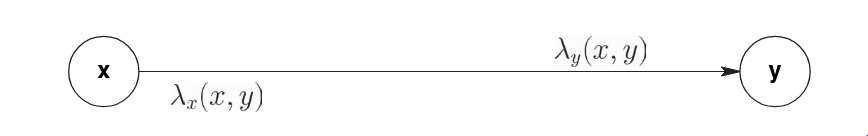
\includegraphics[width=0.8\linewidth]{images/orientation.png}
        \caption{Ciascun arco ha due etichette.}
        \label{fig:orientation}
    \end{figure}

    In generale, $\lambda_x(x, y) \neq \lambda_y(x, y)$.
\end{description}

\subsection{Resitrizioni}
Spesso i protocolli vengono definiti e studiati assumendo ulteriori restrizioni. Naturalmente
un protocollo definito sotto un gran numero di restrizioni è generalmente debole, nel senso
che, rimuovendo alcune di queste restrizioni, il protocollo potrebbe non risolvere il problema
preso in analisi. Un protocollo definito su un sistema con poche restrizioni invece risulta più
generale, e dunque più forte.

Si elencano alcune tipologie di restrizioni.

\begin{description}
    \item[Message Ordering] Si assume che i messaggi inviati da un nodo $x$ a un nodo $y$ arrivino in ordine FIFO (First In First Out) (\textbf{FIFO queue}). Ciò significa che se $x$ invia due messaggi $m_1$ e $m_2$ a $y$, con $m_1$ inviato prima di $m_2$, allora $y$ riceverà $m_1$ prima di $m_2$. Questa restrizione semplifica la progettazione dei protocolli, poiché garantisce un ordine prevedibile dei messaggi tra coppie di nodi.
    \item[Bidirectional Links] Si assume che le connessioni tra nodi sia \textit{bidirezionale}, ossia, $\forall x
    , y \in \mathcal{E}$, se $(x, y) \in E$, allora anche $(y, x) \in E$ e inoltre $\lambda_x(x, y) = \lambda_y(y, x)$. Questa restrizione implica che se un nodo $x$ può inviare messaggi a un nodo $y$, allora $y$ può anche inviare messaggi a $x$, e che entrambi i nodi condividono la stessa etichetta per identificare la connessione tra di loro. Questa restrizione semplifica la progettazione dei protocolli, poiché garantisce una comunicazione simmetrica tra i nodi. Formalmente, 
    \[
        \forall x \in V,\ N_{\text{out}}(x) = N_{\text{in}}(x) = N(x) \quad \text{e} \quad \lambda_x(x, y) = \lambda_y(y, x) \quad \forall y \in N_{\text{out}}(x)
    \]
    \begin{figure}[ht!]
        \centering
        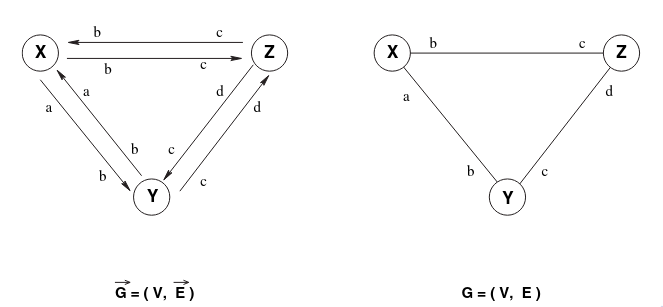
\includegraphics[width=0.8\linewidth]{images/bidirectional.png}
        \caption{In una rete con archi bidirezionali, consideriamo il corrispondente grafo semplificato non diretto.}
        \label{fig:bidirectional}
    \end{figure}
    \item[Reliability Restrictions] Ci chiediamo: cosa succede al messaggio durante il traggitto? Possiamo fare delle assunzioni sulla disponibilità dei canali di comunicazione. 
    \begin{itemize}
        \item \textbf{Guaranteed Delivery}: Ogni messaggio che viene inviato viene \textbf{ricevuto correttamente}, cioè non ci sono corruzioni di messaggi. Sotto questa restrizione, i protocolli non devono tenere conto di omissioni o corruzioni dei messaggi durante la trasmissione.
        \item \textbf{Partial Reliability}: Non si verificano guasti (ad esempio crash dei nodi, perdità di messaggi) dall'istante in cui si inizia ad osservare il sistema. Si osserva che, negli istanti precendenti all'inzio dell'osservazione, il sistema potrebbe aver subito guasti.
        \item \textbf{Total Reliability}: Non sono mai avvenuti fallimenti e mai avverranno in futuro.
    \end{itemize}
    \item[Topological Restrictions] In genere consistono in assunzioni sulla topologia del grafo della rete. Ad esempio assumere che il grafo sia \textbf{connesso/fortemente connesso}.
    \item[Knowledge Restrictions] Assumiamo quali sono le informazioni che ogni nodo conosce riguardo la rete. Ad esempio in numero di nodi ($|V| = n$), oppure il numero di archi ($|E| = m$), il diametro della rete, l'etichettamento universale, etc... .
    \item[Time Restrictions] Eccetto il tempo di trasmissione finito, il modello generale non fa assunzioni su tale quantità.
    Due possibili restrizioni riguardo i tempi di comunicazione sono le seguenti:
    \begin{itemize}
        \item \textbf{Bounded Communication Delay:} Esiste una costante $\Delta$ tale che, in assenza di guasti, il delay dei messaggi è al più $\Delta$, in altre parole se un nodo $x$ invia un messaggio $m$ ad un nodo $y$, $m$ arriverà ad $y$ in al più $\Delta$ istanti di tempo.
        \item \textbf{Syncronized Clock:} Tutti i nodi condividono un clock globale sincronizzato, ossia, $\forall x, y \in \mathcal{E}$, $clock_x(t) = clock_y(t)$ per ogni istante di tempo $t$. Questa restrizione semplifica la progettazione dei protocolli, poiché consente ai nodi di coordinare le loro azioni basandosi su un riferimento temporale comune.
    \end{itemize}
    \item[Cost \& Complexity Measures] In generale in un sistema distribuito non ha senso parlare di complessità temporale, poiché non è detto che i nodi condividano un clock globale. Per parlare di complessità temporale è necessario assumere la \textit{Syncronized Clock} e la \textit{Bounded Communication Delay}. 
    
    Parleremo spesso di \textbf{messagge complexity}, ovvero una misura che tiene conto del numero di messaggi scambiati durante l'esecuzione di un protocollo. Parleremo quindi di numero di bit scambiati, o di numero di messaggi scambiati.
\end{description}

\chapter{Broadcast}

Il primo esempio di comunicazione tra processi è il \textit{broadcast}. Consideriamo un sistema distribuito dove un'entità ha una qualche informazione da condividere con tutte le altre entità. Il processo di inviare un messaggio a tutti gli altri processi è chiamato \textit{broadcast}.

Sia $\mathcal{E}$ l'insieme di tutte le entità nel sistema distribuito e sia $G = (V, E)$ il grafo che rappresenta la rete di comunicazione, dove $V = \mathcal{E}$ e $E$ è l'insieme degli archi che rappresentano le interconnessioni tra i nodi.

Prima di procedere con l'algoritmo di broadcast, è importante assumere alcune restrizioni sul sistema distribuito:
\begin{description}
    \item[Bidirectional Links (BL):] Consideriamo un grafo non diretto, dove ogni arco rappresenta una connessione bidirezionale tra due nodi.
    \item[Total Reliability (TR):] Assumiamo che i messaggi inviati tra i nodi siano sempre consegnati senza errori o perdite.
    \item[Connectivity (CN):] Il grafo $G$ è connesso, il che significa che esiste un percorso tra ogni coppia di nodi nel grafo. Questa assunzione è fondamentele per garantire la risoluzione del problema di broadcast, poiché se il grafo non fosse connesso, alcuni nodi non potrebbero ricevere il messaggio.
    \item[Unique Initiator (UI):] Supponiamo che ci sia un unico nodo che inizia il processo di broadcast, chiamato \texttt{initiator}. Questo nodo è responsabile di inviare il messaggio iniziale a tutti gli altri nodi.
\end{description}

Formalmente, il problema di broadcast può essere definito come segue: dato un grafo $G = (V, E)$ e un nodo $s \in V$ che è l'initiator, l'obiettivo è garantire che ogni nodo $v \in V$ riceva un messaggio da $s$. 

Definiamo l'insieme $\Sigma = \{\texttt{initiator}, \texttt{idle}, \texttt{informed}\}$ come l'insieme di tutti gli stati che può assumere un nodo $x \in \mathcal{E}$.

Definiamo ora le configurazioni del sistema. Una configurazione $C$ è una funzione che associa a ogni nodo $x \in \mathcal{E}$ uno stato in $\Sigma$. Inizialmente, la configurazione $C_{init}$ è tale che esiste unico nodo $s \in V$ tale che $C_{init}(s) = \texttt{initiator}$ e $C_{init}(x) = \texttt{idle}$ per ogni nodo $x \in V \setminus \{s\}$. Il numero di configurazioni iniziali possibili è
\[
    \binom{n}{1} = n,
\]
dove $n$ è il numero di nodi nel grafo. Questo perché possiamo scegliere qualsiasi nodo come initiator.

L'unica configurazione finale accettabile è quella in cui ogni nodo $x \in V$ è nello stato \texttt{informed}, ovvero
\[
    C_{final}(x) = \texttt{informed} \quad \forall x \in V.
\]

Quindi, il problema del broadcast si formalizza mediante la quadrupla:
\[
    \langle \mathcal{R},\ \Sigma,\ C_{init},\ C_{final} \rangle,
\]
dove $\mathcal{R} = \{\texttt{BL, TR, CN, UI}\}$ è l'insieme delle restrizioni, $\Sigma$ è l'insieme degli stati, $C_{init}$ è la configurazione iniziale e $C_{final}$ è la configurazione finale desiderata.

\section{Algoritmo Flooding}

L'idea generale dell'algoritmo di broadcast è quella di utilizzare un approccio di flooding, dove ogni nodo che riceve il messaggio lo inoltra a tutti i suoi vicini. L'algoritmo può essere descritto come segue:
\begin{algorithm}[H]
\caption{Algoritmo di Broadcast (Flooding)}
    \begin{algorithmic}
    \If{$C(s) = \texttt{initiator}$}
        \State $C(s) \gets \texttt{informed}$
        \ForAll{$v \in N(s)$}
            \State send($m$, $v$)
        \EndFor
    \EndIf
    \State
    \If{$C(x) = \texttt{idle}$}
        \State $m \gets$ receive() 
        \State $C(x) \gets \texttt{informed}$
        \ForAll{$v \in N(x) \setminus \{\texttt{sender}\}$}
            \State send($m$, $v$)
        \EndFor
    \EndIf
    \State
    \If{$C(x) = \texttt{informed}$}
        \State do\_nothing()
    \EndIf
    \end{algorithmic}
\end{algorithm}

Descritto in questa maniera, l'algoritmo di flooding risolve il task nella maniera corretta, e dimostreremo inoltre che termina in un tempo finito. Tuttavia, è importante notare che questo algoritmo non è efficiente in termini di complessità di messaggi, poiché ogni nodo potrebbe ricevere lo stesso messaggio più volte da diversi vicini, portando a un numero esponenziale di messaggi inviati.

\textbf{Osservazione.} Se non considerassimo l'insieme degli stati $\Sigma = \{\texttt{initiator}, \texttt{idle}\}$ e non avessimo la condizione che un nodo non inoltra il messaggio se è già informato, l'algoritmo di flooding potrebbe non terminare, poiché i nodi continuerebbero a inoltrare il messaggio indefinitamente.

\begin{lemma}
L'algoritmo di flooding termina in un tempo finito. Sia $\texttt{diam}(G)$ il diametro del grafo $G$, ovvero la massima distanza tra due nodi qualsiasi nel grafo. 

Esiste un tempo massimo $\tau$ tale che tutti i nodi $x$ a distanza $h$ da $s$ ricevano il messaggio $m$ entro il tempo $\tau$.
\[
    \forall h \leq \texttt{diam}(G),\ \exists \tau \in \mathbb{R}^{+}:\ \forall x \in V\ |\ dist(x,s) = h \implies C_{final}(x) = \texttt{informed} \land t(x) \leq \tau.
\]

\begin{proof}
Dimostriamo il lemma per induzione su $h$.
\begin{description}
    \item[Passo Base $\mathbf{h = 1}$] Sfruttando la condizione di Total Reliability, ogni nodo $v$ adiacente a $s$ riceve il messaggio $m$ entro un tempo finito $\tau_1$. Quindi, per ogni nodo $v$ tale che $dist(v, s) = 1$, abbiamo $C_f(v) = \texttt{informed}$ e $t(v) \leq \tau_1$.
    \item[Passo Induttivo $\mathbf{h + 1}$] Sfruttando la condizione di Connectivity, per ogni nodo $x \in V \setminus \{s\}:\ d(s, x) = h + 1$. 
    
    Questo implica che esiste un shortest path $P$ da $s \to x$ di lunghezza $h + 1$. Sia $y$ il nodo adiacente a $x$ su questo percorso, quindi $dist(y, s) = h$. Per ipotesi induttiva, esiste un tempo finito $\tau_h$ tale che $C_{final}(y) = \texttt{informed}$ e $t(y) \leq \tau_h$. 
    
    Sfruttando nuovamente la condizione di Total Reliability, il nodo $x$ riceve il messaggio da $y$ entro un tempo finito $\tau_{h+1}$, quindi $C_{final}(x) = \texttt{informed}$ e $t(x) \leq \tau_{h+1}$.
\end{description}
\end{proof}

\end{lemma}

\begin{lemma}[Message Complexity]
    L'algoritmo di flooding ha una message complexity 
    \[
        M[\texttt{Flooding}] = \theta(|E|) = \theta(m).
    \]
    \begin{proof}
        Dimostriamo il lemma utilizzando due metodi differenti. Nel primo metodo facciamo un'analisi diretta del numero di messaggi inviati, mentre nel secondo metodo utilizziamo un'analisi basata sui nodi e sui loro vicini.
        \begin{description}
            \item[Metodo I: ] L'idea è di contare il numero di messaggi che attraversano un arco. Se $state(s) = \texttt{initiator}$, il numero di messaggi che passano attraverso i suoi archi incidenti è esattamento $1$, ossia solo il messaggio $m$ da inoltrare. Consideriamo adesso due nodi $x \neq s$ e $y \neq s$ adiacenti e contiamo il numero di messaggi che passano attraverso l'arco $(x, y)$. Siano $t_x$ e $t_y$ gli istanti di tempo in cui $x$ e $y$ ricevono il messaggio $m$, e consideriamo il caso in cui $t_x < t_y$. In questo caso, $x$ inoltra il messaggio $m$ a $y$. Tuttavia, al tempo $t_y$, $y$ riceve una copia del messaggio da un nodo $z \neq x$ un'istante prima di riceverlo da $x$. In questo caso, $y$ inoltra il messaggio a $x$. Quindi, il numero massimo di messaggi che passano attraverso l'arco $(x, y)$ è $2$. Quindi ogni arco può essere attraversato da al massimo $2$ messaggi, dimostrando che $M[\texttt{Flooding}] = \theta(2|E|) = \theta(m)$.
            \item[Metodo II: ] Una dimostrazione più precisa può essere ottenuta considerando il numero di messaggi inviati da ogni nodo. Se $state(s) = \texttt{initiator}$, il numero di messaggi inviati è esattamente $d(s)$ dove $d(x) = N(x)$ è il grado di $x$. Consideriamo adesso un nodo $x \neq s$. Il numero di messaggi che invia è $d(x) - 1$, poiché non inoltra il messaggio al nodo da cui lo ha ricevuto. Quindi, il numero totale di messaggi inviati è
            \begin{align*}
                M[\texttt{Flooding}] &= d(s) + \sum_{x \neq s} (d(x) - 1) \\ 
                &= \sum_{x \in V} d(x) - \sum_{x \in V \setminus \{s\}} (n - 1) \\
                &= 2|E| - (n - 1) = 2m - n + 1 = \theta(m).
            \end{align*}
        \end{description}
    \end{proof}
    \textbf{Osservazione.} La somma degli gradi di tutti i nodi in un grafo è pari a $2|E|$, poiché ogni arco contribuisce al grado di due nodi.
\end{lemma}

\subsection{Complessità Temporale}

In generale, non ha senso calcolare la complessità temporale di un algoritmo in un sistema asincronom a causa dell'impossibilità di poter predire i tempo di trasmissione dei messaggi. Tuttavia, se assumiamo un sistema sincrono, ossia assumiamo \textbf{clock sincronizzati} e \textbf{bounded delay}, possiamo calcolare la complessità temporale dell'algoritmo di flooding. Assumiamo che i messaggi vengano trasmessi con un delay di $\delta$ (normalizzando, $\delta = 1$). Chiaramente, il messaggio inviato dall'initiator $s$ deve raggiungere ogni nodo $x$ a distanza $h$ da $s$ entro un tempo finito, e il tempo necessario per raggiungere il nodo più lontano da $s$ è dato \textbf{eccentricity} di $s$, che è definita come
\[
    ecc(s) = \max_{x \in V} dist(s, x).
\]
Allora, nel caso peggiore, il tempo necessario per raggiungere ogni nodo è dato dal diametro del grafo $\texttt{diam}(G)$, che è definito come
\[
    \texttt{diam}(G) = ecc(s).
\]
In conclusione, la complessità temporale \textit{ideale} dell'algoritmo di flooding è
\[
    T[\texttt{Flooding}] = \max_{x \in V} dist(s, x) \leq \texttt{diam}(G) \leq n - 1 = O(n).
\]
Si vuole dimostrare inoltre che tale protocollo sia ottimali in termini di complessità temporale, ossia che non esiste un protocollo di broadcast che possa raggiungere ogni nodo in un tempo minore del diametro del grafo. È necessario quindi dare una delimitazione inferiore alla complessità temporale di qualsiasi protocollo di broadcast. Si osserva che ciascuna entità $x$ a distanza $h$ da $s$ non può ricevere il messaggio $m$ prima di $h$ unità di tempo, poiché il messaggio deve attraversare almeno $h$ archi per raggiungere $x$. Quindi, la complessità temporale di qualsiasi protocollo di broadcast è limitata inferiormente da
\[
    T[\texttt{Broadcast}] \geq \max_{x \in V} dist(s, x) = ecc(s) \leq \texttt{diam}(G).
\]
Di conseguenza, l'algoritmo di flooding è ottimale in termini di complessità temporale, in particolare l'ideal time complexity è $T[\texttt{Flooding}] = \theta(\texttt{diam}(G))$.

\subsection{Stati ed Eventi}

Nel mondo centralizzato, dato uno stesso input ad un algoritmo deterministico, esso non solo genera lo stesso output, ma la sequenza di azioni che svolge per raggiungere tale output è sempre la stessa, ad ogni esecuzione.
Questo dettaglio non vale nel mondo distribuito. Ad esempio nel protocollo flooding, dato che il ritardo dei messaggi varia in modo indeterminato, la sequenza di azioni verso l'unica configurazione finale varia ad ogni esecuzione, anche a fronte di una stessa configurazione iniziale (cioè esecuzioni dallo stesso iniziatore). Naturalmente, per la correttezza del protocollo, una qualsiasi sequenza di azioni anche se diversa converge verso la configurazione finale.

Consideriamo il seguento grafo $G$ con $n = 3$ nodi e $m = 3$ archi, dove $x$ è l'initiator:
\begin{center}
    \begin{tikzpicture}
        \node[circle, draw] (x) at (1, 1.5) {$x$};
        \node[circle, draw] (y) at (0, 0) {$y$};
        \node[circle, draw] (z) at (2, 0) {$z$};
        \draw (x) -- (y);
        \draw (y) -- (z);
        \draw (z) -- (x);
    \end{tikzpicture}
\end{center}

Eseguendo una prima volta il protocollo, supponiamo che $z$ riceva il messaggio da $x$ prima di $y$.

\begin{figure}[ht!]
    \centering
    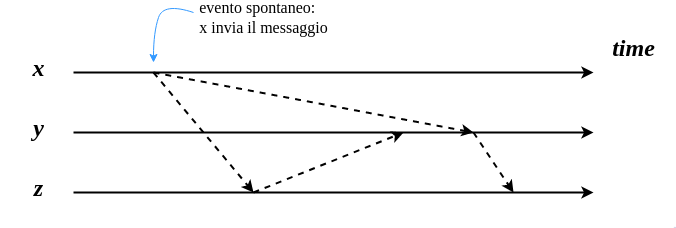
\includegraphics[width=0.6\linewidth]{images/seq1.png}
    \caption{Sequenza di azioni del protocollo di flooding, con $z$ che riceve il messaggio da $x$ prima di $y$.}
    \label{fig:seq1}
\end{figure}

Tale esecuzione può essere rappresentata mediante il seguente grafo, dove ogni nodo rappresenta una configurazione del sistema e ogni arco rappresenta un evento (cioè, l'invio o la ricezione di un messaggio). In questo caso, la sequenza di azioni è $x \to z \to y$.

\begin{center}
    \begin{tikzpicture}
        \node[circle, draw] (x) at (1.5, 0) {$x$};
        \node[circle, draw] (z) at (3, 0) {$z$};
        \node[circle, draw] (y) at (4.5, 0) {$y$};
        \draw[->] (x) -- (z);
        \draw[->] (z) -- (y);
    \end{tikzpicture}
\end{center}

Eseguendo una seconda volta il protocollo, potrebbe capitare che i ritardi sugli archi $(x,z)$ e $(z,y)$ siano simili. Perciò, una possibile sequenza di azione potrebbe essere:

\begin{figure}[ht!]
    \centering
    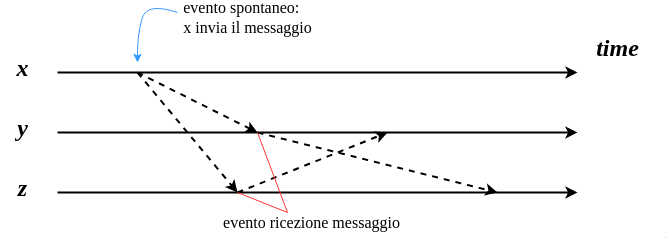
\includegraphics[width=0.6\linewidth]{images/seq2.png}
    \caption{Esecuzione del protocollo con ritardi simili sugli archi $(x,z)$ e $(z,y)$.}
    \label{fig:seq2}
\end{figure}

Tale esecuzione può essere rappresentata mediante il seguente grafo,

\begin{center}
    \begin{tikzpicture}
        \node[circle, draw] (x) at (1, 1.5) {$x$};
        \node[circle, draw] (y) at (0, 0) {$y$};
        \node[circle, draw] (z) at (2, 0) {$z$};
        \draw[->] (x) -- (y);
        \draw[->] (x) -- (z);
    \end{tikzpicture}
\end{center}

Dato che il grafo di comunicazione è sostanzialmente un albero ricoprente, ci sono quindi $O(n^n)$ possibili sequenze di trasmissioni (o \textbf{traiettorie}) che portano alla configurazione finale, anche a fronte di una stessa configurazione iniziale.

\subsection{Lowerbound alla Message Complexity}

\begin{definizione}[Stato Locale Interno]
    Definiamo $\sigma(x, t)$ come lo stato locale interno del nodo $x$ al tempo $t$. Di conseguenza $$\Sigma(t) = \{\sigma(x, t) :\ x \in \mathcal{E} \}$$ è l'insieme di tutti gli stati locali dei nodi al tempo $t$.
\end{definizione}
Consideriamo adesso due ambienti \textit{(environments)} $E_1$ e $E_2$ dove, lo stato interno di $x$ al tempo $t$ è lo stesso, ossia $\sigma_1(x, t) = \sigma_2(x, t)$. Allora $x$ non è in grado di \textit{distinguere} tra i due ambienti. Di conseguenza, se avviene lo stesso evento in entrambi gli ambienti, $x$ esegue la stessa azione in entrambi gli ambienti.

Segueno due proprietà fondamentali che ci permettono di dimostrare un lowerbound alla message complexity di qualsiasi protocollo di broadcast.
\begin{description}
    \item[Proprietà 1:] Se $x$ si trova in due ambienti $E_1$ e $E_2$, e lo stato interno di $x$ è lo stesso in entrambi gli ambienti al tempo $t$ ($\sigma_1(x, t) = \sigma_2(x, t)$), allora $x$ non è in grado di distinguere tra i due ambienti.
    \item[Proprietà 2:] Se due nodi distinti $x$ e $y$ ad un certo istante $t$ si trovano nello stesso stato interno ($\sigma(x, t) = \sigma(y, t)$), allora se vengono sollecitati dallo stesso evento, eseguiranno la stessa azione.
\end{description}

\begin{teorema}[Lower Bound]
    Sotto le ipotesi
    \[
    R = \{\texttt{BL, TR, CN, UI}\} 
    \]
    (ossia, bidirectional links, total reliability, connectivity e unique initiator), qualsiasi protocollo di broadcast ha una message complexity $M[\texttt{Broadcast}] = \Omega(m)$.
    \begin{proof}
        Supponiamo per assurdo che esista un protocollo di broadcast con una message complexity $M[\texttt{Broadcast}] = o(m)$ (per esempio $m-1$ messaggi). Consideriamo un grafo $G = (V, E)$, e sia $s$ l'initiator. Poiché il protocollo ha una message complexity sublineare, esiste almeno un arco $e = (x, y) \in E$ che non viene attraversato da alcun messaggio durante l'esecuzione del protocollo. Sia ora $G' = (V', E')$ costruito a partire da $G$ rimuovendo l'arco $e$ e aggiungengo un nuovo nodo $z$ tale per cui $state(z) = \texttt{idle}$ connesso a $x$ e $y$ mediante due nuovi archi, ossia
        \[
        V' = V \cup \{z\}, \quad E' = E \setminus \{e\} \cup \{(x, z), (y, z)\}.
        \]
        Siano quindi $E_1$ e $E_2$ i due ambienti, dove in $E_1$ il protocollo viene eseguito su $G$, mentre in $E_2$ il protocollo viene eseguito su $G'$.
        Le etichette degli archi in $G$ e $G'$ sono le stesse, quindi $x$ e $y$ non sono in grado di distinguere tra i due ambienti. 
        \[
            \lambda_x(x, y) = \lambda_x(x, z), \quad \lambda_y(y, x) = \lambda_y(y, z).
        \]
        \begin{figure}[ht!]
            \centering
            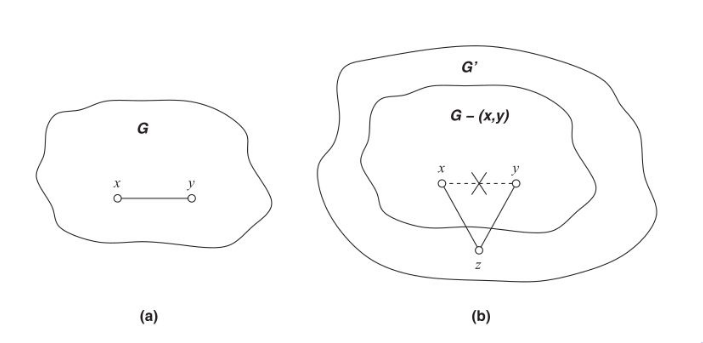
\includegraphics[width=0.8\linewidth]{images/lowerbound.png}
            \caption{Costruzione del grafo $G'$ a partire da $G$.}
            \label{fig:lowerbound}
        \end{figure}
        Allora sapendo che $x$ e $y$ non sono in grado di distinguere (\textbf{Proprietà 1}) tra i due ambienti, se viene sollecitato lo stesso evento in entrambi gli ambienti, $x$ e $y$ eseguono la stessa azione (\textbf{Proprietà 2}). Poiché in $E_1$ non inoltrano il messaggio sul arco $(x, y)$, in $E_2$ non inoltrano il messaggio né su $(x, z)$ né su $(y, z)$. Di conseguenza, il nodo $z$ non riceve mai il messaggio (poiché è collegato solo a $x$ e $y$), e quindi il protocollo di broadcast fallisce in $E_2$, portando ad una contraddizione, ossia vengono inviati $o(m)$ messaggi e rimane un nodo non raggiungibile.
    \end{proof}
\end{teorema}

\textbf{Osservazione.}
Se consideriamo una fase di preprocessing, ossia una fase iniziale in cui i nodi possono scambiarsi messaggi per costruire una mappa della rete (uno \textbf{spanning tree}), allora è possibile progettare un protocollo di broadcast con una message complexity $M[\texttt{Broadcast}] = O(n)$, che è ottimale in quanto ogni nodo deve ricevere almeno un messaggio. Tuttavia, in questo caso, la message complexity totale del protocollo (preprocessing + broadcast) è $M[\texttt{Total}] = O(n + m) = O(m)$, che è ancora ottimale in quanto ogni arco deve essere attraversato da almeno un messaggio durante la fase di preprocessing.


\chapter{Spanning Tree Construction}

\begin{definizione}[Spanning Tree]
    Un albero ricoprente (Spanning Tree) di un grafo $G = (V, E)$ è un sottografo connesso e aciclico di $G$ tale che $T = (V, E')$ dove $E' \subseteq E$ . In altre parole è un albero che include tutti i nodi di $V$.
\end{definizione}

\begin{definizione}[SPT Construction Distributed Problem]
    In un sistema distribuito, il problema di costruire un albero ricoprente (Spanning Tree) del grafo $G = (V, E)$ significa portare il sistema da uno stato iniziale, in cui ogni nodo è consapevole solo di se stesso e dei suoi vicini, a uno stato finale in cui tutti i nodi sono organizzati in una struttura ad albero che copre tutti i nodi del grafo. In altre parole,
    \begin{description}
        \item[Configurazione Iniziale:] Ciascun nodo $x \in \mathcal{E} = V$ mantiene una struttura dati $\texttt{tree\_neigh(x)} = \emptyset$. La possiamo immaginare come un vettore binario, dove ogni posizione rappresenta un nodo vicino ad $x$, e il valore 1 indica che l'arco tra $x$ e quel nodo è parte dell'albero, mentre 0 indica che non lo è.
        \item[Configurazione Finale:] $\forall x \in \mathcal{E} = V$, 
        \[
            \texttt{tree\_neigh(x)} = \{\text{archi che appartengono allo ST}\},
        \]
        e l'unione di tutti questi insiemi per  forma un albero ricoprente del grafo $G$. 
    \end{description}
\end{definizione}

Il problema è formalizzato dalla triplia $P = \langle P_{init}, P_{final}, R \rangle$, dove:
\begin{description}
    \item[$P_{init}$] = $\forall x \in V$, 
    \begin{align*}
        &\texttt{tree\_neigh(x)} = \emptyset \\
        &\exists! s \in V,\ state(s) = \texttt{initiator} \\
        &\forall x \in V \setminus \{s\},\ state(x) = \texttt{idle}
    \end{align*}
    \item[$P_{final}$] = $\forall x \in V$, 
    \begin{align*}
        &\texttt{tree\_neigh(x)} = \{y \in N(x): (x, y) \in E'\} \\
        &\bigcup_{x \in V} \texttt{tree\_neigh(x)} = T(V, E') \text{ albero ricoprente del grafo } G \\
        &\forall x \in V,\ state(x) = \texttt{done}
    \end{align*}
    \item[$R$] = $\{\texttt{TR, BL, CN, UI}\}$
\end{description}

Quindi, a differenza di un algorimo centrallizzato (Kruskal, Prim), la conoscenza dello ST è distribuita tra i nodi, e ogni nodo deve collaborare con i suoi vicini per costruire l'albero ricoprente. Non esiste quindi una visiione globale dell'albero, ma ogni nodo deve basarsi solo sulle informazioni locali e sui messaggi ricevuti dai suoi vicini per decidere se includere o meno un arco nel suo insieme $\texttt{tree\_neigh(x)}$.

\section{Single Source SHOUT Protocol}

L'idea dell'algoritmo è quella di chiedere ai nodi vicini se sono interessati a far parte dello ST, e se sì, includere l'arco che li collega al nodo che ha fatto la richiesta. In questo modo, partendo da un nodo iniziale (initiator), si costruisce gradualmente lo ST coinvolgendo i nodi vicini.

Definiamo $\Sigma = \{\texttt{initiator}, \texttt{idle}, \texttt{active}, \texttt{done}\}$ dove $S_{init} = \{\texttt{initiator}, \texttt{idle}\}$ l'insieme dei stati iniziali e $S_{final} = \{\texttt{done}\}$ l'insieme dei stati finali.

\begin{itemize}
    \item Inizialmente, tutti i nodi tranne l'iniziatore $s$ sono in stato \texttt{idle}, e $s$ è in stato \texttt{initiator}. Spontaneamnete, $s$ si sveglia e invia i messaggi di domanda (\texttt{Q}) a tutti i suoi vicini, proponendo loro di essere connessi a lui nello ST (cioè essere suoi figli).
    \item Quando un nodo $x$ nello stato \texttt{idle} riceve un messaggio \texttt{Q}, questo si attiva, sceglie come padre il \textbf{primo} nodo da cui ha ricevuto il messaggio e invia a tale nodo il messaggio \texttt{YES}.
    \item Successivamente, $y$ invia a tutti i suoi vicini, tranne il padre, un messaggio \texttt{Q} per chiedere se vogliono essere suoi figli. Se un nodo $z$ nello stato \texttt{active} riceve un messaggio \texttt{Q} da $y$, risponde con un messaggio \texttt{NO} perché ha già scelto un padre e non può accettare più di uno. Se invece $z$ è nello stato \texttt{idle}, risponde con un messaggio \texttt{YES} e si attiva, scegliendo $y$ come padre.
    \item Ogni nodo conta il numero di risposte ricevute da suoi vicini. Quando un nodo $x$ ha ricevuto risposte da tutti i suoi vicini, passa allo stato \texttt{done} e non fa più nulla.
\end{itemize}

Per un nodo $x$, i vicini che rispondono con \texttt{YES} saranno inclusi nel suo insieme \\ $\texttt{tree\_neigh(x)}$ includendo anche il vicino che ha fatto la richiesta.

Possimo quindi considerare il protocollo SHOUT come un broadcast con reply.

\begin{algorithm}[H]
\caption{Algoritmo di SHOUT}
    \begin{algorithmic}
    \If{state(x) = \texttt{initiator}} spontaneously
        \State root $\gets$ true
        \State \texttt{tree\_neigh(x)} $\gets \emptyset$
        \State state(x) $\gets$ \texttt{active}
        \State counter $\gets 0$
        \ForAll{$v \in N(x)$}
            \State send(\texttt{Q}, $v$)
        \EndFor
    \EndIf
    \State
    \If{state(x) = \texttt{idle}}
        \State $\texttt{Q} \gets$ receive()
        \State \texttt{tree\_neigh(x)} $\gets \{ \texttt{sender} \}$
        \State root $\gets$ false
        \State counter $\gets 1$
        \State send(\texttt{YES}, \texttt{sender})
        \If {counter $= |N(x)|$}
            \State state(x) $\gets$ \texttt{done}
        \Else        
            \ForAll{$v \in N(x) \setminus \{\texttt{sender}\}$}
                \State send($\texttt{Q}$, $v$)
            \EndFor
            \State state(x) $\gets$ \texttt{active}
        \EndIf
    \EndIf
    \State
    \If{state(x) = \texttt{active}}
        \State $\texttt{reply} \gets$ receive()
        \If {reply = \texttt{YES}}
            \State \texttt{tree\_neigh(x)} $\gets$ \texttt{tree\_neigh(x)} $\cup$ \{\texttt{sender}\}
            \State counter $\gets$ counter + 1
            \If {counter $= |N(x)|$}
                \State state(x) $\gets$ \texttt{done}
            \EndIf
        \EndIf
        \State
        \If {reply = \texttt{NO}}
            \State counter $\gets$ counter + 1
            \If {counter $= |N(x)|$}
                \State state(x) $\gets$ \texttt{done}
            \EndIf
        \EndIf
        \State
        \If {reply = \texttt{Q}}
            \State send(\texttt{NO}, \texttt{sender})
        \EndIf
    \EndIf
    \end{algorithmic}
\end{algorithm}

\begin{figure}[ht!]
    \centering
    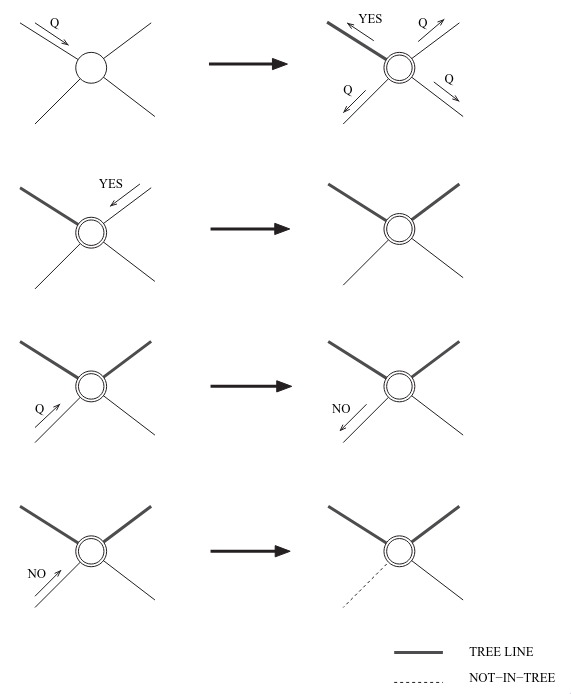
\includegraphics[width=0.5\linewidth]{images/shout.png}
    \caption{Insieme di regole del protocollo SHOUT.}
    \label{fig:shout}
\end{figure}

\subsection{Terminazione}
Il protocollo SHOUT è molto simile al protocollo di broadcast con l'aggiunta dei messaggi di reply \texttt{YES} e \texttt{NO}. Poiche siamo sotto le assunzioni \texttt{TR} e \texttt{CN}, allora ogni nodo $x \neq s$ riceverà entro un tempo finito un messaggio \texttt{Q} da un vicino, e quindi si attiverà impostando il contatore a 1 (per la correttezza del protocollo di broadcast). Per ogni richiesta ricevuta, i nodi risponderanno con un messaggio \texttt{YES} o \texttt{NO}, di conseguenza, ogni nodo riceverà (per la \texttt{TR} e per la costruzione del protocollo, ogni nodo risponderà a tutte le richieste) un numero finito di risposte ($|N(x)|$), e quindi, entro un tempo finito, ogni nodo raggiungerà lo stato \texttt{done}, terminando localmente la popria esecuzione.

\subsection{Correttezza}

Per dimostrare la correttezza del protocollo SHOUT, dobbiamo mostrare che alla fine dell'esecuzione, l'insieme di archi scelti da tutti i nodi forma un albero ricoprente del grafo $G$.

\begin{lemma}[Coerenza]\label{lemma:coerenza}
    Siano $x$ e $y$ due nodi vicini in $G$. Se $x$ ha come vicino $y$ in ST, cioè $y \in \texttt{tree\_neigh(x)}$, allora $x$ è vicino di $y$ in ST, cioè $x \in \texttt{tree\_neigh(y)}$. Quindi 
    \[
        \forall x, y \in V,\ y \in \texttt{tree\_neigh(x)} \iff x \in \texttt{tree\_neigh(y)}.
    \]
    \begin{proof}
        Supponiamo che $y \in \texttt{tree\_neigh(x)}$. Allora $y$ ha risposto con un messaggio \texttt{YES} alla richiesta di $x$, e quindi $y$ ha scelto $x$ come padre. Ma se $y$ ha riposto con \texttt{YES} a $x$, allora $y$ era nello stato \texttt{idle} quando ha ricevuto la richiesta da $x$ e per definizione del protocollo $y$ inserisce $x$ nel suo insieme $\texttt{tree\_neigh(y)}$. Quindi $x \in \texttt{tree\_neigh(y)}$. La dimostrazione dell'implicazione inversa è simile, con $x$ e $y$ scambiati.
    \end{proof} 
\end{lemma}

\begin{lemma}[Connettività/Spanning]\label{lemma:spanning}
    Il sottografo $T = (V, E')$ definito da 
    \[
        E' = \bigcup_{x \in V} \texttt{tree\_neigh(x)}
    \]
    è connesso e include tutti i nodi di $V$. In altre parole, il sottografo indotto dagli archi su cui è viaggiato il messaggio \texttt{YES} è connesso e include tutti i nodi di $V$ (è ricoprente e connesso).
    \begin{proof}
        Vogliamo dimostrare che per ogni nodo $x \in V \setminus \{s\}$, se $x$ ha risposto \texttt{YES} ad un nodo $y$, allora $x \in \texttt{tree\_neigh(y)}$, dove quest'ultimo è connesso alla sorgente $s$ tramite una sequenza di archi sui quali sono passati i messaggi \texttt{YES}, e tale sequenza formerà un cammino da $s \to x$.
        
        Sia $x$ un nodo qualsiasi in $V \setminus \{s\}$. Se $x$ ha risposto \texttt{YES} ad un nodo $y$, allora $x \in \texttt{tree\_neigh(y)}$, e dato che $y$ deve aver inviato una proposto al nodo $x$, allora $y$ si trova in \texttt{active} alla ricezione della risposta \texttt{YES} da $x$. Ma $y$ invia una proposta al nodo $x$ solo se:
        \begin{itemize}
            \item $y$ è la sorgente $s$, e quindi è connesso a se stesso, oppure
            \item $y$ ha ricevuto una proposta da un nodo $z$ e ha risposto \texttt{YES} a $z$, e quindi $y$ è connesso a $z$ tramite un arco su cui è passato un messaggio \texttt{YES}, quindi 
            \[
            z \in \texttt{tree\_neigh(y)} \text{ e } y \in \texttt{tree\_neigh(z)} \qquad \autoref{lemma:coerenza}
            \]
            Iterando questo processo fino alla sorgente $s$, si ottiene un cammino che collega $s$ a $x$ tramite archi su cui sono passati messaggi \texttt{YES}, e quindi $x$ è connesso a $s$.
        \end{itemize}
    \end{proof}
\end{lemma}

\begin{lemma}[Aciclicità]\label{lemma:acyclicity}
    Il sottografo $T = (V, E')$ definito da 
    \[
        E' = \bigcup_{x \in V} \texttt{tree\_neigh(x)} \text{ è aciclico}.
    \]
    \begin{proof}
        Supponiamo per assurdo che $T$ contenga un ciclo. Allora esiste una sequenza di nodi $v_1, v_2, \ldots, v_k$ con $k \geq 3$ tale che $(v_i, v_{i+1}) \in E'$ (ossia $v_i$ è padre di $v_{i+1}$) per ogni $i = 1, 2, \ldots, k-1$ e $(v_k, v_1) \in E'$. 

        Poichè ogni nodo, eccetto la sorgente invia \textbf{un solo} messaggio \texttt{YES}, allora il ciclo $v_1, v_2, \ldots, v_k$ non contiene la sorgente $s$. Per il \autoref{lemma:spanning}, deve esistere un cammino da $s$ a qualsiasi nodo, inclusi quelli de ciclo. Ma poiché deve esistere un cammino da $s$ a $v_i$, allora esiste un cammino da $s$ a $v_i$ che passa attraverso il ciclo, il che implica che esiste un cammino da $s$ a $v_i$ che contiene un ciclo. Questo è una contraddizione, poiché un cammino non può contenere un ciclo. Quindi, il sottografo $T$ deve essere aciclico.
    \end{proof}
\end{lemma}

\begin{teorema}
    Il protocollo SHOUT costruisce un albero ricoprente del grafo $G$.
    \begin{proof}
        Dal \autoref{lemma:spanning} sappiamo che il sottografo $T$ è connesso e include tutti i nodi di $V$, e dal \autoref{lemma:acyclicity} sappiamo che $T$ è aciclico. Quindi, combinando questi due risultati, possiamo concludere che $T$ è un albero ricoprente del grafo $G$.
    \end{proof}
\end{teorema}

\subsection{Message Complexity}

Come menzionato sopra, il protocollo \texttt{SHOUT = Flood + Reply}. Quindi la complessità in termini di messaggi consiste nell'esecuzione di \texttt{Flood(Q)} più le risposte \texttt{YES} o \texttt{NO} per ogni richiesta ricevuta. In altre parole,
\[
    M[\texttt{SHOUT}] = M[\texttt{Flood(Q)} + \texttt{Reply}] = 2M[\texttt{Flood(Q)}] = O(4|E|) = O(|E|).
\]
Più precisamente, i messaggi inviati dal protocollo possono essere divisi in due categorie: \texttt{Q} e \texttt{Reply} = \{ \texttt{YES}, \texttt{NO} \}. Di conseguenza, abbiamo le seguenti casistiche:
\begin{itemize}
    \item Per ogni arco $(x, y) \in ST$ costruito dal protocollo passano due messaggi: un messaggio \texttt{Q} inviato da $x$ a $y$ e un messaggio \texttt{YES} inviato da $y$ a $x$. Il numero di archi sono $|E'| = |V| - 1$, quindi il numero di messaggi in questa categoria è $2(|V| - 1) = 2(n - 1)$.
    \begin{center}
        \begin{tikzpicture}[
            node distance=3cm, 
            every node/.style={circle, draw, minimum size=0.6cm, thick},
            arrow style/.style={-{Stealth[scale=1.2]}, thick}
        ]

        \node (A) {};
        \node (B) [right of=A] {};

        \draw[thick] (A) -- (B);

        \draw[arrow style] (A) to [bend left=45] node[draw=none, above, text=red] {Q} (B);

        \draw[arrow style] (B) to [bend left=45] node[draw=none, below, text=red] {YES} (A);
        \end{tikzpicture}
    \end{center}
    \item Per ogni arco $(x, y) \in E \setminus ST$ passano quattro messaggi: due messaggi \texttt{Q} in entrambe le direzioni, seguiti da due messaggi \texttt{NO} in entrambe le direzioni. Il numero di archi in questa categoria è $|E| - |E'| = |E| - (|V| - 1)$, quindi il numero di messaggi in questa categoria è $4(|E| - (|V| - 1)) = 4(m - n + 1)$.
    \begin{center}
        \begin{tikzpicture}[
            node distance=3cm, 
            every node/.style={circle, draw, minimum size=0.6cm, thick},
            arrow style/.style={-{Stealth[scale=1.2]}, thick}
        ]

        \node (A) {};
        \node (B) [right of=A] {};
        \node (C) [right of=B] {};
        \node (D) [right of=C] {};

        \draw[thick] (A) -- (B);
        \draw[thick] (C) -- (D);

        \draw[arrow style] (A) to [bend left=45] node[draw=none, above, text=red] {Q} (B);
        \draw[arrow style] (B) to [bend left=45] node[draw=none, below, text=red] {Q} (A);
        \draw[arrow style] (C) to [bend left=45] node[draw=none, above, text=red] {NO} (D);
        \draw[arrow style] (D) to [bend left=45] node[draw=none, below, text=red] {NO} (C);
        \end{tikzpicture}
    \end{center}
\end{itemize}

\textbf{Osservazione.} Su ogni arco $(x, y)$ non potranno mai passare le coppie di messaggi (\texttt{NO}, \texttt{YES}) e (\texttt{YES}, \texttt{YES}).

\begin{description}
    \item [(\texttt{NO}, \texttt{YES})] Non può accadere in quanto il nodo sinitro per rispondere a \texttt{NO} deve prima aver ricevuto una richiesta dal nodo destro, ma per inviare una richiesta, il nodo destro deve avere già un padre, dunque non può rispondere con \texttt{YES} a nessuna richiesta.
    \item [(\texttt{YES}, \texttt{YES})] Non può accadere in quanto due nodi per inviarsi reciprocamente un messaggio \texttt{YES} devono essersi entrambi inviati reciprocamente un messaggio \texttt{Q}, ma ciò implica che hanno già un padre, e quindi hanno già risposto con un messaggio \texttt{YES} a un altro nodo.
\end{description}

\begin{center}
        \begin{tikzpicture}[
            node distance=3cm, 
            every node/.style={circle, draw, minimum size=0.6cm, thick},
            arrow style/.style={-{Stealth[scale=1.2]}, thick}
        ]

        \node (A) {};
        \node (B) [right of=A] {};
        \node (C) [right of=B] {};
        \node (D) [right of=C] {};

        \draw[thick] (A) -- (B);
        \draw[thick] (C) -- (D);

        \draw[arrow style] (A) to [bend left=45] node[draw=none, above, text=red] {NO} (B);
        \draw[arrow style] (B) to [bend left=45] node[draw=none, below, text=red] {YES} (A);
        \draw[arrow style] (C) to [bend left=45] node[draw=none, above, text=red] {YES} (D);
        \draw[arrow style] (D) to [bend left=45] node[draw=none, below, text=red] {YES} (C);
        \end{tikzpicture}
    \end{center}

Quindi, il numero totale di messaggi è:
\[\]
\[
    M[\texttt{SHOUT}] = 2(n - 1) + 4(m - n + 1) = 4m - 2n + 2 = O(|E|).
\]

\newpage
\section{Single Source SHOUT+ Protocol}

Si osserva che nel protocollo SHOUT, i messaggi di risposta \texttt{NO} non sono necessari per far sapere al nodo che ha inviato la richiesta quando entrare nello stato \texttt{done}. Infatti, se un nodo $y$ invia \texttt{NO} ad $x$, allora $y$ ha inviato un messaggio \texttt{Q} ad $x$ prima dell'invio di \texttt{NO}, in quanto $y$ per inviare \texttt{NO} deve trovarsi nello stato \texttt{active}, e per trovarsi nello stato \texttt{active}, il nodo $y$ deve avere già scelto un nodo come padre e aver mandato il messaggio \texttt{Q} a tutti i suoi vicini. Dunque il nodo $x$ può interpretare il messaggio \texttt{Q} inviato da $y$ come un messaggio \texttt{NO}, e quindi non è necessario inviare un messaggio \texttt{NO} esplicito. 

In questa maniera, la message complexity del protocollo SHOUT si riduce a 
\[
    M[\texttt{SHOUT+}] = 2(n - 1) + 2(m - n + 1) = 2m = O(|E|).
\]

Riguardo la terminazione locale del protocollo, ogni nodo sa che il suo compito è terminato nel momento in cui passa nello stato \texttt{done}. Sarebbe interessante sapere se un nodo è in grado di capire quanto il processo termina globalmente, cioè quando tutti i nodi sono nello stato \texttt{done}. Certamente, se la sorgente è $s$ è in grado di sapere quanto lo spanning tree è completato, allora potrebbe mandare una notifica in broadcast a tutti i nodi e avvertirli della terminazione globale. Il problema è che ogni nodo ha solamente una \textbf{visione locale} della rete in cui si trova, perciò a meno che non ci sia un nodo che riesca ad osservare lo stato della rete dall'alto non è possibile sapere solo col protocollo \texttt{SHOUT/SHOUT+} quando il processo è terminato globalmente.

\textbf{Osservazione.} Osserviamo che anche nel caso della costruzione dello spanning tree, il lower bound $\Omega(m)$ è rispettato, in quanto per costruire lo spanning tree è necessario che ogni nodo riceva almeno un messaggio da ogni vicino, e quindi è necessario che ogni arco venga attraversato da almeno un messaggio.

\textbf{Osservazione.} Si può osservare che lo spanning tree costruito dal protocollo \texttt{SHOUT/SHOUT+} dipende fortemente dalla singola esecuzione e non dal protocollo, in quanto i ritardi di trasmissione variano ogni volta. Ciò implica che maneggiando adeguatamente i ritardi di trasmissione potrebbe accadere che $diam(ST) >> diam(G)$.

\begin{teorema}
    L'esecuzione di ogni protocollo di \texttt{Broadcast} costuisce uno spanning tree \textbf{entrante} (ogni nodo possiede solamente informazioni su chi è il nodo padre, generando un albero orientato verso la radice) del grafo $G$.
    \begin{proof}
        Diamo un'idea della dimostrazione. Definiamo
        \[
        father(x) = \text{ il nodo dal quale } x \text{ ha ricevuto per primo il messaggio } m
        \]
        Allora, se consideriamo l'ordinamente \textit{parziale} $father(x) > x$ otteniamo uno spanning tree entrante, con radice $s$.
    \end{proof}
\end{teorema}

\begin{algorithm}[H]
\caption{Algoritmo di SHOUT}
    \begin{algorithmic}
    \If{state(x) = \texttt{initiator}} spontaneously
        \State root $\gets$ true
        \State \texttt{tree\_neigh(x)} $\gets \emptyset$
        \State state(x) $\gets$ \texttt{active}
        \State counter $\gets 0$
        \ForAll{$v \in N(x)$}
            \State send(\texttt{Q}, $v$)
        \EndFor
    \EndIf
    \State
    \If{state(x) = \texttt{idle}}
        \State $\texttt{Q} \gets$ receive()
        \State \texttt{tree\_neigh(x)} $\gets \{ \texttt{sender} \}$
        \State root $\gets$ false
        \State counter $\gets 1$
        \State send(\texttt{YES}, \texttt{sender})
        \If {counter $= |N(x)|$}
            \State state(x) $\gets$ \texttt{done}
        \Else        
            \ForAll{$v \in N(x) \setminus \{\texttt{sender}\}$}
                \State send($\texttt{Q}$, $v$)
            \EndFor
            \State state(x) $\gets$ \texttt{active}
        \EndIf
    \EndIf
    \State
    \If{state(x) = \texttt{active}}
        \State $\texttt{reply} \gets$ receive()
        \If {reply = \texttt{YES}}
            \State \texttt{tree\_neigh(x)} $\gets$ \texttt{tree\_neigh(x)} $\cup$ \{\texttt{sender}\}
            \State counter $\gets$ counter + 1
            \If {counter $= |N(x)|$}
                \State state(x) $\gets$ \texttt{done}
            \EndIf
        \EndIf
        \State
        \If {reply = \texttt{Q}}
            \State counter $\gets$ counter + 1
            \If {counter $= |N(x)|$}
                \State state(x) $\gets$ \texttt{done}
            \EndIf
        \EndIf
    \EndIf
    \end{algorithmic}
\end{algorithm}

\newpage

\section{Multiple Sources Spanning Tree Construction}

Supponiamo ora di avere più nodi \texttt{initiator}, ossia che 
\[
    \exists I \subseteq V,\ |I| > 1 \text{ e } \forall s \in I,\ state(s) = \texttt{initiator}.
\]
In questo scenario, l'insieme delle restrizioni diventa $R = \{\texttt{TR, BL, CN}\}$

\begin{teorema}\label{th:MultipleSourcesST}
    Sotto le assunzioni $R = \{\texttt{TR, BL, CN}\}$, il problema della costruzione di spanning tree con multipli \texttt{initiator} non è deterministicamente risolvibile.
    \begin{proof}
    Consideriamo una clique di 3 nodi $x, y, z$, tutti e tre \texttt{initiator}. Consideriamo il caso sincrono in cui tutti si attivano e iniziano il protocollo al tempo $t_0$.

    \begin{center}
        \begin{tikzpicture}
            \node[circle, draw] (x) at (1, 1.5) {$x$};
            \node[circle, draw] (y) at (0, 0) {$y$};
            \node[circle, draw] (z) at (2, 0) {$z$};
            \draw (x) -- (y);
            \draw (y) -- (z);
            \draw (z) -- (x);
        \end{tikzpicture}
    \end{center}
    Sappiamo che se prendiamo dei nodi aventi lo stesso stato interno $\sigma(v, t)$, allora essi da quel momento in poi si comporteranno allo stesso modo, dato che nessuno è in grado di distinguire una loro \textit{identità} all'interno della rete. In questo caso, al tempo $t_0$, abbiamo che $\sigma(x, t_0) = \sigma(y, t_0) = \sigma(z, t_0) = \texttt{initiator}$, e quindi $x, y, z$ si comporteranno allo stesso modo. Quindi ciascun nodo invierà un messaggio \texttt{Q} ed entrerà nello stato \texttt{active}. Quando  riceveranno un messaggio \texttt{Q} da ciascuno dei loro vicini, risponderanno con un messaggio \texttt{NO} a ciascuno dei loro vicini, e quindi entreranno nello stato \texttt{done}. Quindi, alla fine dell'esecuzione, avremo che 
    \[
        \texttt{tree\_neigh(x)} = \texttt{tree\_neigh(y)} = \texttt{tree\_neigh(z)} = \emptyset,
    \]
    e quindi non è stato costruito alcun albero ricoprente del grafo $G$.
    \end{proof}
\end{teorema}

Per risolvere questo problema è necessario risolvere un'altro problema: il problema della \textbf{leader election}. Eletto un leader tra tutti i nodi \texttt{initiator}, esso potrà eseguire uno dei protocolli di costruzione di spanning tree a singola sorgente già noti.

Vedremo in futuro che il problema della leader election può essere risolto in maniera deterministica solamente se i nodi sono univocamente identificati in maniera globale
\chapter{Wake-Up Problem}

Il problema del wake-up è un problema nel mondo dei sistemi distribuiti che riguarda un insieme di nodi iniziali \textit{svegli (attivi)} che devono svegliare un insieme di nodi \textit{dormienti (inattivi)} tramite lo scambio di messaggi. Il problema del wake-up è una generalizzazione del problema del broadcast, in cui non c'è un solo nodo \texttt{initiator}, bensì un sottoinsieme di nodi.

Formalmente, il problema del wake-up può essere definito come segue, dalla quadrupla $\langle P_{init}, P_{final}, R, \Sigma \rangle$, e sia $W \subseteq V$ l'insieme di \texttt{initiator} tale che $W \neq \emptyset$:
\begin{description}
    \item[$P_{init}$] = $\forall x \in V$
    \[
        state(x) =
        \begin{cases}
            \texttt{awake} & \texttt{ if } x \in W \\
            \texttt{asleep} & \texttt{ if } x \in V \setminus W
        \end{cases}
    \]
    \item[$P_{final}$] = $\forall x \in V,\ state(x) = \texttt{awake}$
    \item[$R$] = $\{\texttt{TR, BL, CN}\}$
    \item[$\Sigma$] = \{\texttt{awake}, \texttt{asleep}\} 
\end{description}

\textbf{Osservazione.} Se il numero di nodi $|V| = n$, allora il numero possibile di configurazioni iniziali $|P_{init}| = 2^n - 1$ (insieme vuoto). Quindi l'avversario è in grado di scegliere tra $2^n - 1$ configurazioni iniziali una volta visto il grafo della rete, oltre a poter ritardare a piacere le trasmissioni.

\begin{algorithm}[H]
\caption{Algoritmo WFlood}
\begin{algorithmic}
    \If {state(x) = \texttt{awake}} spontaneamente
        \ForAll{$y \in N(x)$}
           \State \texttt{send}(\texttt{wake-up}, $y$)
        \EndFor
    \EndIf
    \If {state(x) = \texttt{asleep} $\wedge$ \texttt{receive}(\texttt{wake-up}, $sender$)}
        \State state(x) $\gets$ \texttt{awake}
        \ForAll{$z \in N(x) \setminus \{sender\}$}
           \State \texttt{send}(\texttt{wake-up}, $z$)
        \EndFor
    \EndIf
    \end{algorithmic}
\end{algorithm}

\section{Analisi dell'algoritmo WFlood}

\subsection{Correttezza}

La correttezza dell'algoritmo WFlood segue dalla correttezza dell'algoritmo di flooding. Di seguito è riportata una dimostrazione formale:
\begin{teorema}
    Esiste un tempo $t \in \mathbb{R}^+$ tale che $\forall x \in V, state(x) = \texttt{awake}$, ossia che al tempo $t$, $W \equiv V$.
    \begin{proof}
        Consideriamo $W \subset V$ sottoinsieme proprio. Se $ W = V $, allora il tempo di terminazione dell'algoritmo è $t = 0$. Definiamo ora la distanza di un nodo dall'insieme $W$ come
        \[
            d(x, W) = \min_{y \in W} d(x, y)
        \]
        Per definizione del protocollo, sappiamo che a un certo punto tutti i nodi che sono nello stato \texttt{awake} avranno inviato il messaggio a tutti i vicini, e data l'assunzione di \texttt{TR}, possiamo essere certi che esiste un tempo finito $t_1$ entro il quale tutti i nodi a distanza $1$ da $W$ avranno ricevuto il messaggio. Definiamo quindi l'insieme
        \[
            L_1 = \{x \in V: d(x, W) = 1\}
        \]
        Supponiamo per \textit{ipotesi induttiva} che questo valga per una qualsiasi distanza $d > 1$, ossia che esiste un tempo $t_d$ tale che tutti i nodi in $L_d$ sono nello stato \texttt{awake}. Consideriamo un nodo $x \in L_{d + 1}$. Osserviamo che poichè $x \in L_{d + 1}$, allora deve esistere un nodo $y \in L_{d-1}$ tale per cui $(y, x) \in E$. Se così non fosse, allora ogni cammino minimo da $W$ arriverebbe in $x$ tramite un arco $(z, x)$ tale che $z \in L_k$ con $k \neq d$, e ciò implica che $x$ è a distanza $k + 1 \neq d + 1$, ovvero che $x \not \in L_{d+1}$. 

        Dato che $y$ è stato informato entro il tempo $t_d$, per definizione del protocollo $y$ invierà \texttt{wake-up} a tutti i suoi vicini, compreso $x$. Grazie alla \texttt{TR}, siamo certi che questo messaggio arriverà entro un tempo finito $t_{d+1}$. Quindi possiamo concludere che $\exists\ t_{d+1}$ tempo finito entro il quale $\forall x \in L_{d+1},\ state(x) = \texttt{awake}$.
    \end{proof}
\end{teorema}

\subsection{Message Complexity}

Sia $k = |W|$ il numero di nodi iniziali nello stato \texttt{awake}. Ogni nodo in $W$ invia un messaggio a tutti i suoi vicini, mentre ogni nodo in $V \setminus W$ invia un messaggio a tutti i suoi vicini eccetto il \texttt{sender}. Dunque, il numero totali di messaggi sono:

\begin{align*}
    M[\texttt{WFlood}] 
    &= \sum_{u \in W} |N(u)| + \sum_{u \in V \setminus W} (|N(u)| - 1) \\ 
    &= \sum_{u \in W} |N(u)| + \sum_{u \in V \setminus W} |N(u)| - \sum_{u \in V \setminus W}1 \\
    &= \sum_{u \in V} |N(u)| - \sum_{u \in V \setminus W} 1 \\
    &= 2m - (n - k) = 2m + n - k 
\end{align*}

\textbf{Osservazione.} Osserviamo che il caso peggiore è quando $k = n$, ossia che $W \equiv V$. In questo caso il numero di messaggi è esattamente $2m$. Viceversa, il caso migliore è quando il $|W| = 1$ (come nel broadcast) e il numero di messaggi è $2m - n + 1$. Vale quindi la seguente relazione:

\[
    M[\texttt{WFlood}/R] \geq 
    M[\texttt{Broadcast}R_{\texttt{bcast}}] = \Omega(m)
\]

Questo dimostra ancora che il problema del \textbf{wake-up} è una generalizzazione del problema del broadcast.

\subsection{Ideal Time Complexity}

Consideriamo il nuovo insieme di restrizioni
\[
    R = R\ \cup\ \{\texttt{Syncronized Clock, Bounded Communication Delay}\}
\]
allora possiamo calcolare il tempo di terminazione ottimale. Abbiamo osservato che il caso $|W| = n$ rappresenta il worst-case scenario nel caso della message complexity. Per quanto riguarda il costo temporale, il caso peggiore è quando $|W| = 1$, infatti in questo caso abbiamo che
\[
    T[\texttt{Broadcast}R_{\texttt{bcast}}] = T[\texttt{WFlood}/R] = O(\texttt{diam}(G))
\]

\textbf{Osservazione.} Se consideriamo il problema del wake-up su un albero, allora è vero che
\[
M[\texttt{WFlood/Tree}] = 2m - n + k = 2(n - 1) - n + k = n + k - 2
\]

\section{Lower Bound su Clique (Da FARE)}
\chapter{Labeled Hypercube}

Generalmente, in un contesto reale si cuole costruire reti che abbiano le seguenti proprietà:
\begin{itemize}
    \item \textbf{Diametro piccolo}, $O(1)$ oppure PolyLog$(n)$, in modo da ridurre i tempi di comunicazione tra i nodi.
    \item \textbf{Grado piccolo}, in modo da ottenre grafi \textbf{sparsi}, che sono più facili da costruire e mantenere.
\end{itemize}

Il principale vantaggio di un grafo sparso è la sua \textbf{scalabilità}, ovvero la capacità di crescere senza un aumento troppo grande del numero di link. Per esempio una \textit{clique} non è molto scalabile, perché se aggiunto un nuovo nodo, è necessario aggiungere altri $n-1$ link. Al contrario, se consideriamo un grafo a \textit{lista}, osserviamo che è facilmente scalabile, in quanto il grado di ciascun nodo è $2$, indipendentemente dal numero di nodi presenti. Tuttavia, il diametro di un grafo a lista è $O(n)$ (mentre il diametro di una clique è $O(1)$), il che lo rende poco efficiente per la comunicazione tra nodi distanti.

Quindi osserviamo che esiste un trade-off tra diametro e grado: se vogliamo un diametro piccolo, dobbiamo accettare un grado più grande, e viceversa. Un grafo ideale sarebbe quello che riesce a mantenere sia un diametro piccolo che un grado piccolo.

Consideriamo un altro esempio di grafo, il \textit{grafo a griglia}. In questo grafo, i nodi sono disposti in una \textbf{griglia bidimensionale}, e ogni nodo è connesso ai suoi vicini immediati. Il grado di ogni nodo è al massimo 4 (a meno che non si trovi ai bordi della griglia), e il diametro del grafo è $O(\sqrt{n})$, il che è un miglioramento rispetto al grafo a lista, ma ancora non è ideale.

\section{Broadcast su Labeled Hypercube}

Vogliamo quindi studiare il problema del broadcast in un grafo che abbia sia un diametro piccolo che un grado piccolo. Un esempio di tale grafo è l'\textbf{ipercubo etichettato} (labeled hypercube), che ha un diametro di $O(\log n)$ e un grado di $O(\log n)$, rendendolo una scelta interessante per la costruzione di reti scalabili ed efficienti.

Consideriamo l'insieme delle restrizioni 
\[
    R = \{\texttt{TR, BL, CN, UI, KN}\}
\]
dove \texttt{KN} è l'assunzione di \textbf{knowledge}, ovvero che ogni nodo la struttura della rete in cui si trova, ossia un \textbf{labeled hypercube} di dimensione $d$.

\subsection{Costruzione Hypercube}

\begin{definizione}[Hamming Distance]
    La \textbf{Hamming distance} tra due stringhe binarie $\bar{x}$ e $\bar{y}$ di lunghezza $d$, denotata come $h_d(\bar{x}, \bar{y})$, è il numero di posizioni in cui le due stringhe differiscono. Formalmente, se $\bar{x} = x_1 x_2 \ldots x_d$ e $\bar{y} = y_1 y_2 \ldots y_d$, allora:
    \[
    h_d(\bar{x}, \bar{y}) = |\{i : 1 \leq i \leq d, x_i \neq y_i\}|
    \]
\end{definizione}

\begin{definizione}[Labeled Hypercube]
    Definiamo la struttura \textbf{labeled hypercube} $\mathcal{H}_d$ di dimensione $d$ come un grafo $\mathcal{H}_d(V, E)$, dove:
    \begin{itemize}
        \item $V = \{0, 1\}^d \implies n = |V| = 2^d$. Ciascun nodo è univocamente identificato da una stringa (\textbf{label}) binaria di lunghezza $d$.
        \item $E = \{(\bar{x}, \bar{y}) : \bar{x}, \bar{y} \in V: h_d(\bar{x}, \bar{y}) = 1\} \implies m = |E| = \frac{n \cdot d}{2} = \frac{n \log_2n}{2}$. Due nodi sono connessi da un arco se e solo se differiscono in esattamente una posizione (ovvero, hanno un Hamming distance di 1).
        
        Inoltre, ogni arco è etichettato con l'indice della posizione in cui i due nodi differiscono. Ad esempio, se $\bar{x} = 000$ e $\bar{y} = 001$, allora l'arco tra $\bar{x}$ e $\bar{y}$ è etichettato con $3$, poiché differiscono solo nella terza posizione.
    \end{itemize}
\end{definizione}

Diremo che $\mathcal{H}_d$ è una struttura quasi sparsa, poiché il numero di archi è $O(n \log n)$, che è maggiore di $O(n)$ (struttura sparsa) ma ancora molto più piccolo di $O(n^2)$ (struttura densa).

\begin{figure}[htbp]
    \centering
    \animategraphics[autoplay,loop,width=0.8\textwidth]{20}{images/hypercube/hypercube-}{1}{280}
    \caption{Animazione di un labeled hypercube di dimensione $d=3$. Aprire con Adobe Reader oppure Okular.}
    \label{fig:hypercube}
\end{figure}

\textbf{Osservazione.} Il labeled hypercube è un grafo molto scalabile. Infatti si può estendere un ipercubo di dimensione $d$ con un altro ipercubo di dimensione $d$, semplicemente aggiungendo un arco tra i nodi analoghi dei due ipercubi.

\begin{figure}[htbp]
    \centering
    \begin{subfigure}[b]{0.3\textwidth}
        \centering
        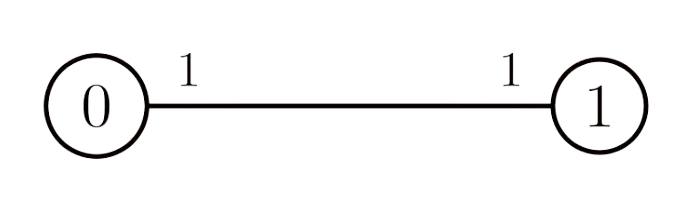
\includegraphics[width=\textwidth]{images/d1.png}
        \caption{Labeled Hypercube di dimensione $d=1$.}
        \label{fig:labelled_hypercube_d1}
    \end{subfigure}
    \hfill
    \begin{subfigure}[b]{0.3\textwidth}
        \centering
        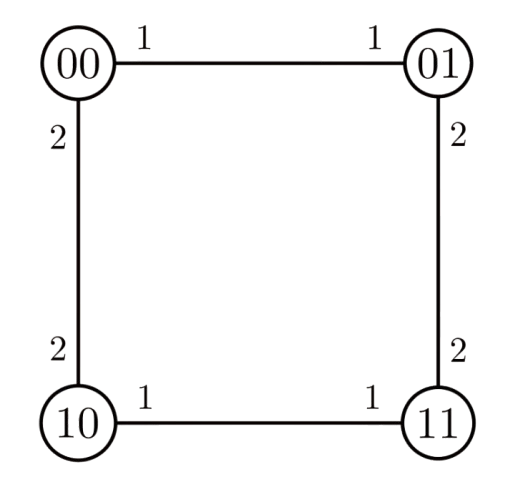
\includegraphics[width=\textwidth]{images/d2.png}
        \caption{Labeled Hypercube di dimensione $d=2$.}
        \label{fig:labelled_hypercube_d2}
    \end{subfigure}
    \hfill
    \begin{subfigure}[b]{0.3\textwidth}
        \centering
        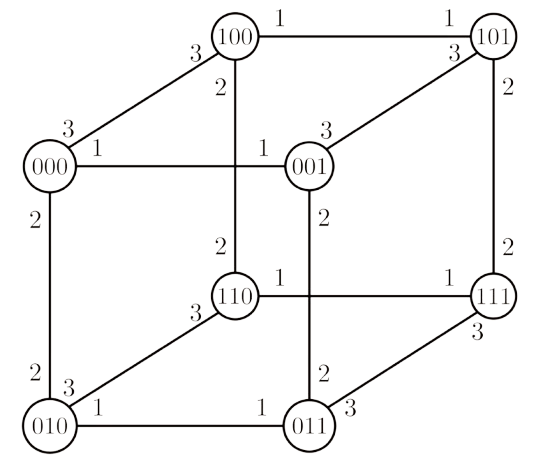
\includegraphics[width=\textwidth]{images/d3.png}
        \caption{Labeled Hypercube di dimensione $d=3$.}
        \label{fig:labelled_hypercube_d3}
    \end{subfigure}
\end{figure}

\newpage

\begin{teorema}
    Sia $\mathcal{H}_d$ un labeled hypercube di dimensione $d$. Allora:
    \begin{enumerate}
        \item $\delta(\bar{x}) = d = \log_2 n \quad \forall \bar{x} \in V$
        \item $diam(\mathcal{H}_d) = d = \log_2 n$
    \end{enumerate}
    \begin{proof}
        Dimostriamo ciascuna affermazione separatamente:
        \begin{enumerate}
            \item Poichè $|V| = 2^d$, e ogni nodo ha come vicini a distanza di hamming 1, allora ogni nodo ha esattamente $d$ vicini.
            \item Per dimostrare che il diametro è $d$, dobbiamo mostrare che $\forall \bar{x}, \bar{y} \in V$, esiste un cammino $P = (\bar{x} = \bar{v_0}, \bar{v_1}, \ldots, \bar{v_k} = \bar{y})$ tale che $k \leq d$. Siano quindi $\bar{x} = x_1 x_2 \ldots x_d$ e $\bar{y} = y_1 y_2 \ldots y_d$ due nodi arbitrari in $V$.
            \begin{itemize}
                \item Se $\bar{x} = \bar{y}$, allora $k = 0 \leq d$.
                \item Se $\bar{x} \neq \bar{y}$, scorrendo gli indici delle due stringhe a partire dalla posizione più significativa (MSB, da sinistra), e confrontando i bit, incontreremo il primo indice $j_1$ tale per cui $x_{j_1} \neq y_{j_1}$. A questo punto, per costruzione dell'ipercubo, esisterà un suo vicino $\bar{x}'$ tale che $x_{j_1}' = y_{j_1}$ e $x_i' = x_i$ per tutti gli altri indici $i$.
                \[
                    \bar{x} = x_1 x_2 \ldots x_{j_1} \ldots x_d \quad \xrightarrow{(j_1)} \quad \bar{x}' = x_1 x_2 \ldots y_{j_1} \ldots x_d
                \]
                Consideriamo quindi l'arco $(\bar{x}, \bar{x}')$ come primo arco del cammino $P$.

                A questo punto, $\forall i \leq j_1$, $x_i' = y_i$, quindi partendo dall'indice $j_1 + 1$ e continuando a scorrere verso sinistra, se arrivati a $d$ e non abbiamo ancora trovato un indice $j_2$ tale che $x_{j_2}' \neq y_{j_2}$, allora $\bar{x}' = \bar{y}$ e il cammino $P$ è completo con $k = 1 \leq d$.
                
                Altrimenti, se esiste un indice $j_2$ tale che $x_{j_2}' \neq y_{j_2}$, allora esisterà un vicino $\bar{x}''$ di $\bar{x}'$ tale che $x_{j_2}'' = y_{j_2}$ e $x_i'' = x_i'$ per tutti gli altri indici $i$.

                Iterando questo processo, alla fine si arriverà ad un nodo $\bar{x}^{(k)}$ tale che $\bar{x}^{(k)} = \bar{y}$, e il cammino $P$ sarà completo con $k \leq d$, poiché in ogni passo ci spostiamo di un bit solo, e al massimo ci sono $d$ bit da modificare per trasformare $\bar{x}$ in $\bar{y}$.
            \end{itemize}
        \end{enumerate}
    \end{proof}
\end{teorema}

\textbf{Osservazione.} Se ci spostiamo da MSB $\to$ LSB, allora il cammino $P$ che abbiamo costruito è un cammino \textbf{crescente}, ovvero un cammino in cui le etichette degli archi sono in ordine crescente. Se invece ci spostiamo da LSB $\to$ MSB, allora il cammino $P$ è un cammino \textbf{decrescente}, ovvero un cammino in cui le etichette degli archi sono in ordine decrescente.

\section{Protocollo Hyperflood}

Il protocollo \textbf{Hypercube Flooding} (Hyperflood) è un algoritmo di broadcast che sfrutta la struttura del labeled hypercube per diffondere un messaggio da un nodo sorgente a tutti gli altri nodi in modo efficiente. Inoltre, viene altamente sfruttata la conoscenza della struttura del grafo (assunzione \texttt{KN}) per ottimizzare la diffusione del messaggio.

L'idea del protocollo è la seguente: l'unico nodo $\bar{s} \in V$ \texttt{initiator} invia il messaggio $m$ a tutti i suoi vicini. Qualsiasi altro nodo $\bar{x} \neq \bar{s}$ riceve il messaggio da un arco etichettato con $l$, allora inoltrerà il messaggio su tutti gli archi 
\[
    \{(\bar{x}, \bar{y}) \in E : l' = \lambda(\bar{x}, \bar{y}) < l\}
\]

\textbf{Osservazione.} Il protocollo sfrutta la struttura gerarchica del labeled hypercube: il nodo iniziatore invia il messaggio ad un nodo all'interno di ogni sotto-ipercubo di dimensione $l' = l - 1$, e ognuno di questi nodi diventa iniziatore del sotto-ipercubo di cui fa parte.

\begin{algorithm}[H]
\caption{Hyperflood}
    \begin{algorithmic}
    \If{state($\bar{x}$) = state($\bar{s}$)} spontaneamente
        \ForAll{$\bar{y} \in N(\bar{x})$}
            \State send($m$, $\bar{y}$)
        \EndFor
    \Else
        \State $\texttt{m}, \texttt{l} \gets$ receive()
        \ForAll{$\bar{y} \in N(\bar{x})$}
            \If{$\lambda(\bar{x}, \bar{y}) < l$}
                \State send($m$, $\bar{y}$)
            \EndIf
        \EndFor
    \EndIf
    \end{algorithmic}
\end{algorithm}

\begin{teorema}[Correttezza]
    Per ogni coppia di nodi $\bar{x}, \bar{y} \in V$, esiste sempre un cammino $P$ con \textbf{etichette decrescenti} da $\bar{x}$ a $\bar{y}$. Nel protollo Hyperflood, il messaggio verrà inoltrato lungo questo cammino.
    \begin{proof}
        La dimostrazione è la stessa del secondo punto del teorema precedente, in quanto il protocollo Hyperflood costruisce esattamente un cammino con etichette decrescenti da $\bar{x}$ a $\bar{y}$.

        Vediamo invece un esempio pratico. Considerimo due nodi $\bar{x} = 100010100$ e $\bar{y} = 110001000$. Consideriamo la procedura per costruire un cammino usata nel secondo punto del teorema precedente, ma partendo da LSB $\to$ MSB, in modo da ottenere un cammino con etichette decrescenti. Consideriamo inoltre gli indici ordinai in modo decresente, allora i due nodi differiscono in posizioni $8, 5, 4, 3$. Allora, un cammino che li collega è formato dagli archi con etichette $8, 5, 4, 3$, ovvero con etichette decrescenti.
        
        \begin{figure}[htbp]
        \centering
        \animategraphics[autoplay,loop,width=0.8\textwidth]{20}{images/correttezza/hypercube-}{1}{280}
        \caption{Animazione costruzione cammino. Aprire con Adobe Reader oppure Okular.}
        \label{fig:correttezza_hyperflood}
    \end{figure}    
    \end{proof}
\end{teorema}

\begin{teorema}[Message Complexity]
    \[
        M[\texttt{Hyperflood}] = n - 1 =  O(n)
    \]
    \begin{proof}
        Per dimostrare che il numero di messaggi è $n - 1$, ossia uno per ogni nodo, mostreremo che il grafo indotto dai archi lungo cui viene trasmesso il messaggio è un \textbf{albero}.

        Supponiamo per assurdo che esiste un nodo $\bar{y}$ che riceve due copie del messaggio. Allora nel grafo delle comunicazioni esistono due cammini \textit{disgiunti} che partono da un nodo $\bar{x}$ (sorgente inclusa) e arrivano a $\bar{y}$.

        Per costruzione dell'ipercubo, i due cammini sono tali per cui i loro rispettivi archi iniziali posseggono due etichette $l_1 \neq l_2$. Senza perdità di generalità, assumiamo $l_1 < l_2$ e che l'arco a sinistra inizi con l'arco etichettato $l_1$ e quello a destra inizi con l'arco etichettato $l_2$. Sia $\bar{x}'$ il nodo raggiunto da $l_1$ e $\bar{x}''$ il nodo raggiunto da $l_2$, come in \autoref{fig:hyperflood_msg_combined}.

        \begin{figure}[ht!]
            \centering
            \begin{subfigure}[b]{0.32\textwidth}
                \centering
                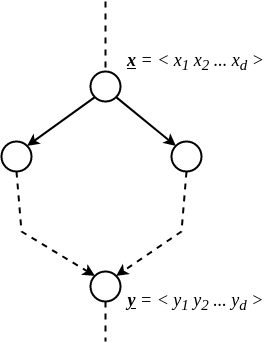
\includegraphics[width=\textwidth]{images/hyperflood_msg_1.png}
                \caption{Due cammini da $\bar{x}$ a $\bar{y}$.}
                \label{fig:hyperflood_msg_1}
            \end{subfigure}
            \hfill
            \begin{subfigure}[b]{0.32\textwidth}
                \centering
                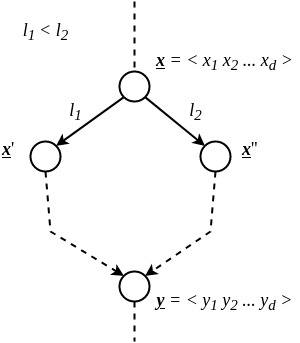
\includegraphics[width=\textwidth]{images/hyperflood_msg_2.png}
                \caption{Archi etichettati $l_1$ e $l_2$.}
                \label{fig:hyperflood_msg_2}
            \end{subfigure}
            \begin{subfigure}[b]{0.32\textwidth}
                \centering
                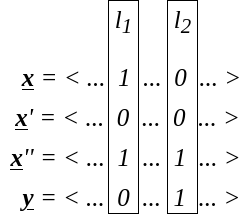
\includegraphics[width=\textwidth]{images/hyperflood_msg_3.png}
                \caption{Posizione dei bit in cui differiscono $\bar{x}$ e $\bar{y}$.}
                \label{fig:hyperflood_msg_3}
            \end{subfigure}
            \caption{Dimostrazione della struttura ad albero nel protocollo Hyperflood.}
            \label{fig:hyperflood_msg_combined}
        \end{figure}

        Per costruzione del cammino, il nodo $\bar{x}$ differisce da $\bar{y}$ almeno per i bit in posizione $l_1$ e $l_2$ (vedere animazione in \autoref{fig:correttezza_hyperflood}).

        Abbiamo quindi che $\bar{x}'$ differisce da $\bar{y}$ per il bit in posizione $l_2$, e $\bar{x}''$ differisce da $\bar{y}$ per il bit in posizione $l_1$. 

        Ci troviamo quindi nella situazione in \autoref{fig:hyperflood_msg_3}. Poiche i cammini procedono per etichette \textbf{decrescenti}, il cammino di sinistra includerà solo i nodi che differiscono da $\bar{x}'$ per i bit in posizione $l_i < l_1$, ma questo implica che il cammino di sinistra porta a $\bar{y}$ senza mai cambiare il bit in posizione $l_2$, ma questo è un \textbf{assurdo} dato che $\bar{x}$ e $\bar{y}$ differiscono per il bit in posizione $l_2$.

        Questo dimostra che nel grafo di comunicazione non ci sono cicli, e quindi è un albero. Di conseguenza, ogni nodo riceve esattamente un messaggio, e il numero totale di messaggi è $n - 1$.
    \end{proof}
\end{teorema}

\begin{teorema}[Ideal Time]
    Sotto le restrizioni 
    \[
    R \cup \{\texttt{Synchronized Clock, Bounded Communication Delay}\}
    \]
    il tempo ideale per il broadcast è $O(\log n)$.
    \begin{proof}
        Dimostrazione per induzione sulla \textit{distanza di Hamming} dei nodi dalla sorgente. Dimostriamo che per ogni $j \geq d$, e per ogni $\bar{x}$ a distanza di Hamming $j$ dalla sorgente, il nodo $\bar{x}$ riceve il messaggio al tempo $j$.

        \[
            \forall j \in [d], \forall \bar{x} \in V = \{0, 1\}^d: h_d(\bar{s}, \bar{x}) = j \implies t_{recv}(\bar{x}) = j
        \]
        Per $j = 1$ è banale, in quanto per definizione del protocollo, la sorgente invia il messaggio a tutti i suoi vicini i quali hanno distanza di Hamming 1 dalla sorgente, e quindi ricevono il messaggio al tempo $t = 1$.

        Definiamo ora $L_j = \{ \bar{x} \in V : h_d(\bar{s}, \bar{x}) = j \}$ e supponiamo per induzione che sia vero per $j - 1$, ovvero che tutti i nodi in $L_{j-1}$ ricevano il messaggio al tempo $t = j - 1$. Sappiamo che per ogni nodo $\bar{x} \in L_j$, esiste un cammino con etichette decrescenti da $\bar{s}$ a $\bar{x}$, allora esiste un nodo $\bar{y} \in L_{j-1}$ tale che $\bar{x}$ è un vicino di $\bar{y}$. Per ipotesi, $\bar{y}$ è già stato informato al tempo $t = j - 1$ e inoltre il messaggio impiega un istante per attraversare l'arco $(\bar{y}, \bar{x})$, quindi $\bar{x}$ riceve il messaggio al tempo $t = j$. 
        Poiché la lunghezza massima di un cammino è $d$, allora ogni nodo riceve il messaggio al tempo $t \leq d = O(\log n)$.
    \end{proof}
\end{teorema}
\chapter{Depth First Traversal (DFT) Protocol}

Consideriamo un problema in cui uno \textit{inziale} possiede un \textbf{token}, e di volere che questo token (non replicabile) venga passato a \textbf{tutti} i nodi dell rete. Possiamo vedere questo problema come un problema di \textit{scheduling/assegnazione} di un compito/risorsa (il token) a più processori (i nodi della rete), dove la risorsa è \textit{mutualmente esclusiva} tra i nodi.

Formalmente, il problema è definito dalla seguente tripla $\langle P_{init}, P_{final}, R \rangle$, dove, sia per ogni nodo $x \in V$, \texttt{received(x)} un registro interno che contiene \texttt{true} se $x$ ha ricevuto il token almeno una volta, e \texttt{false} altrimenti:
\begin{itemize}
    \item $P_{init}: \exists! x \in V$ tale che \texttt{received($x$)} = \texttt{true} e per ogni $y \in V$ con $y \neq x$, \texttt{received($y$)} = \texttt{false}, ossia $x$ è il nodo iniziale che possiede il token.
    \item $P_{final}$ : per ogni $x \in V$, \texttt{received(x)} = \texttt{true}, ossia tutti i nodi hanno ricevuto il token almeno una volta seguendo l'ordine di una DFS.
    \item $R=\{ \texttt{TR, BL, CN, UI} \}$.
\end{itemize}

\section{Protocollo BACK}

Il protocollo più semplice per risolvere questo problema è il protocollo BACK, che funziona come segue:
\begin{enumerate}
    \item Quando un nodo riceve il token per la \textit{prima volta}, ricorda il nodo che gli ha inviato il token (il padre) e inoltra il token ad uno dei suoi vicini non visitati con il messaggio \texttt{token}, aspettando la sua risposta.
    \item  Quando il vicino riceve il token, se lo ha già ricevuto lo ritorna immediatamente con il messaggio \texttt{back\_edge}, altrimenti lo inoltra a tutti i suoi vicini in modo sequenziale, per poi ritornarlo al nodo da cui lo ha ricevuto con il messaggio \texttt{return}.
    \item Alla ricezione di un \texttt{return}, il nodo inoltra il token al vicino successivo non visitato, se esiste, altrimenti lo ritorna al padre con il messaggio \texttt{return}.
\end{enumerate}

\begin{itemize}
    \item $S = \{\texttt{initiator, idle, visited, done}\}$
    \item $S_{init} = \{\texttt{initiator, idle}\}$
    \item $S_{final} = \{\texttt{done}\}$
\end{itemize}

\begin{algorithm}
\caption{Protocollo BACK}
\begin{algorithmic}[1]
    \If{state(x) = \texttt{initiator}} spontaneously
        \State \texttt{unvisited} $\gets N(x)$
        \State \texttt{initiator} $\gets True$
        \State \texttt{visit()}
    \EndIf
    \State
    \If{state(x) = \texttt{idle}}
        \State \texttt{token} $\gets$ \texttt{receive()}
        \State \texttt{parent} $\gets$ \texttt{sender(token)}
        \State \texttt{unvisited} $\gets N(x) \setminus \{\texttt{parent}\}$
        \State \texttt{initiator} $\gets False$
        \State \texttt{visit()}
    \EndIf
    \State
    \If{state(x) = \texttt{visited}}
        \State \texttt{msg} $\gets$ \texttt{receive()}
        \If{\texttt{msg} = \texttt{token}}
            \State \texttt{unvisited} $\gets N(x) \setminus \{\texttt{sender(msg)}\}$
            \State \texttt{send(back\_edge, sender(msg))}
        \ElsIf{\texttt{msg} = \texttt{return}}
            \State \texttt{visit()}
        \ElsIf{\texttt{msg} = \texttt{back\_edge}}
            \State \texttt{visit()}
        \EndIf
    \EndIf
    \State
    \If{state(x) = \texttt{done}}
        \State \texttt{do\_nothing()}
    \EndIf
    \State
    \Procedure{visit}{}
        \If{\texttt{unvisited} $\neq \emptyset$}
            \State \texttt{next} $\gets$ \texttt{pop(unvisited)}
            \State \texttt{send(token, next)}
            \State state(x) $\gets$ \texttt{visited}
        \Else
            \If{\texttt{not initiator}}
                \State \texttt{send(return, parent)}
            \EndIf
            \State state(x) $\gets$ \texttt{done}
        \EndIf
    \EndProcedure
\end{algorithmic}
\end{algorithm}

\begin{teorema}[Message Complexity]
    \[
        M[\texttt{BACK}] = 2m \in \theta(m)
    \]
    \begin{proof}
        Osserviamo che esistono 3 tipologie di messaggi: 
        \begin{itemize}
            \item \texttt{token}, quando un nodo inoltra il token per procedere con la visita.
            \item \texttt{return}, quando un nodo già visitato restituisce il token al padre dopo aver visitato tutti i suoi vicini.
            \item \texttt{back\_edge}, quando un nodo già visitato riceve il token e lo restituisce immediatamente al mittente.
        \end{itemize}
        Inoltre, su ogni arco può passare uno tra i messaggi \texttt{back\_edge} e \texttt{return}, mentre il messaggio \texttt{token} può passare al massimo una volta per ogni arco, quando viene inoltrato per la prima volta. Di conseguenza, il numero totale di messaggi è al massimo $2m \in \theta(m)$. In realtà si dimostra che il lower bound rimane $\Omega(m)$, in quanto non è possibile effettuare il broadcasting di una informazione in meno di $m$ messaggi.
    \end{proof}
\end{teorema}

\begin{teorema}[Ideal Time]
    Sotto le restrizioni 
    \[
    R \cup \{\texttt{Synchronized Clock, Bounded Communication Delay}\}
    \]
    si ha che
    \[
        T[\texttt{BACK}] = \theta(m)
    \]
    \begin{proof}
        Ogni nodo esplora \textbf{sequentialmente} i suoi vicini, e ogni messaggio impiega un tempo costante per essere consegnato. Di conseguenza, il tempo totale è proporzionale al numero di messaggi, che è $\theta(m)$.
    \end{proof}
\end{teorema}
    
\section{Protocollo BACK+}

Il principale difetto del protocollo BACK è che ogni nodo esplora i suoi vicini in modo sequenziale, e questo porta ad un tempo totale di $\theta(m)$. Il protocollo BACK+ migliora questo aspetto, permettendo ad ogni nodo di esplorare i suoi vicini in modo \textbf{parallelo}, e questo porta ad un tempo totale di $\theta(n)$, che è ottimale, aumentando la message complexity di un fattore 2.

\begin{itemize}
    \item Quando un nodo $x$ riceve il token, \textbf{informa} il suo vicinato $N(x)$ che possiede il token, ossia che è stato visitato.
    \item Tutti i nodi in $N(x)$ inviano un messaggio di \texttt{ack} a $x$ per confermare che hanno ricevuto l'informazione.
    \item Dopo aver ricevuto tutti gli \texttt{ack}, $x$ inoltra il token a uno dei suoi vicini non visitati.
\end{itemize}

La differenza sostanziale di questo protocollo è che i \texttt{back\_edges} sono scoperti in parallelo e non più in modo sequenziale.

\begin{teorema}[Message Complexity]
    \[
        M[\texttt{BACK+}] = 4m \in \theta(m)
    \]
    \begin{proof}
        Osserviamo che esistono 4 tipologie di messaggi: 
        \begin{itemize}
            \item \texttt{token}, quando un nodo inoltra il token per procedere con la visita.
            \item \texttt{visited}, qunado un nodo che ha appena ricevuto il token lo notifica ai suoi vicini.
            \item \texttt{ack}, quando un nodo conferma di aver ricevuto l'informazione che il suo vicino è stato visitato.
            \item \texttt{return}, quando un nodo già visitato restituisce il token al padre dopo aver visitato tutti i suoi vicini.
        \end{itemize}
        Ogni nodo (eccetto la sorgente $s$) riceverà \texttt{token} una volta, e invierà \texttt{return} una sola volta, per un totale di $2(n-1)$ messaggi.

        Per quanto riguarda il messaggio \texttt{visited}, ogni nodo lo invierà a tutto il suo vicinato meno che al nodo da cui hanno ricevuto il token. La sorgente sarà l'unico nodo che lo invierà a tutto il suo vicinato, quindi:
        \begin{align*}
            M[\texttt{visited}] &= |N(s)| + \sum_{x \in V \setminus \{s\}} |N(x)| - 1 = \\
            &= |N(s)| + \sum_{x \in V \setminus \{s\}} |N(x)| - \sum_{x \in V \setminus \{s\}} 1 = \\
            &= \sum_{x \in V} |N(x)| - \sum_{x \in V \setminus \{s\}} 1 = 2m - (n-1)
        \end{align*}
        Inoltre, per ogni notifica \texttt{visited} corrisponde un messaggio \texttt{ack}, quindi 
        \[
            M[\texttt{BACK+}] = 2(n-1) + 2(2m - (n-1)) = 4m = 2M[\texttt{BACK}] \in \theta(m)
        \]
    \end{proof}
\end{teorema}

\begin{teorema}[Ideal Time]
    Sotto le restrizioni 
    \[
    R \cup \{\texttt{Synchronized Clock, Bounded Communication Delay}\}
    \]
    si ha che
    \[
        T[\texttt{BACK+}] = \theta(n)
    \]
    \begin{proof}
        Abbiamo che in soli due istanti, ogni nodo invierà le notifiche e riceverà le risposte. Per il tempo necessario al completamento del task sarà:
        \begin{itemize}
            \item $n - 1$ per messaggi inviati di tipo \texttt{return}.
            \item $n - 1$ per messaggi inviati di tipo \texttt{token}.
            \item $n$ per messaggi inviati di tipo \texttt{visited}.
            \item $n$ per messaggi inviati di tipo \texttt{ack}.
        \end{itemize}
        per un totale di $4n - 2 \in \theta(n)$.
    \end{proof}
\end{teorema}

\textbf{Osservazione.} Con questa ottimizzazione, anche se si paga un fattore $2$ alla message complexity, si ottiene un miglioramento significativo del tempo di esecuzione, che passa da $\theta(m)$ a $\theta(n)$, che è ottimale. In particolare, in grafi densi, dove $m$ è dell'ordine di $n^2$, questo miglioramento è particolarmente rilevante.
\chapter{Tree Computations}

Consideriamo adesso una serie di problemi computazionali su alberi. Come possiamo osservare, gli alberi hanno una struttura asimmetrica, e questo ci permette di risolvere alcuni problemi in modo più efficiente e semplice rispetto ai grafi generici o a struttura nelle quali è difficile rompere la simmetria. Infatti, non è necessario utilizzare tecniche di rottura della simmetria, come ad esempio l'assegnazione di ID unici ai nodi, per risolvere problemi su alberi.

Infatti, un nodo all'interno di albero può identificare la propria posizione all'interno della struttura,
\begin{itemize}
    \item Un nodo sa di essere una \textit{foglia} in quanto ha grado 1 ($N(x) = 1$), mentre è un nodo \textit{interno} se ha grado maggiore di 1 ($N(x) > 1$).
        \item Un altra proprietà importante è che ogni tipologia di albero ha almeno due foglie.
        \usetikzlibrary{chains}
        \begin{center}
            \begin{tikzpicture}[start chain=going right, node distance=10mm, every node/.style={on chain, join}, thick]
                \node[circle,draw] {1};
                \node[circle,draw] {2};
                \node[draw=none] {$\dots$};
                \node[circle,draw] {$n$};
            \end{tikzpicture}
        \end{center}
\end{itemize}

Introduciamo la tecnica di \textit{saturazione}, che ci permette di risolvere problemi su alberi in ambiente distribuito in modo efficiente.

\section{Saturation Technique}

Consideriamo un ambiente distribuito con una topologia ad albero e sia tale informazione, riguardante la struttura topologica, nota a tutti i nodi della rete. La tecnica di saturazione consiste nell'identifacare una singola coppia di nodi adiacenti all'interno della rete. Tale coppia di nodi sarà in grado di far iniziare altre computazioni. In pratica, la tecnica di saturazione consiste nell'eleggere un arco della rete. Osserviamo che non c'è nessuna garanzia su quale arco venga eletto: questa tecnica garantisce l'elezione di uno fra i possibili archi, ma non garantisce quale arco venga eletto.

Tipicamente la tecnica di saturazione è usata per risolvere problemi distribuiti di varia natura. In particolare, la saturazione è inserita all'interno di un processo più grande, che può essere diviso nelle seguenti tre fasi:
\begin{itemize}
    \item \textbf{Attivazione}: in questa fase, i nodi iniziatori attivano i restanti nodi della rete utilizzando un protocollo di \texttt{wake-up}.
    \item \textbf{Saturazione}: in questa fase, a partire dalle foglie si identifica un'unica coppia di nodi adiacenti, anche detti \textit{nodi saturati}.
    \item \textbf{Risoluzione}: in questa fase, i nodi saturati danno inizio ad una o più computazioni necessarie alla risoluzione di uno specifico problema distribuito.
\end{itemize}

Ci focalizziamo ora a definire le prime due fasi poiché la terza fase dipende dal problema specifico che si vuole risolvere. Definiamo la tripla $\langle P_{init}, P_{final}, R\rangle$ e sia $T = (V, E)$ l'albero considerato. Sia inoltre $W \subseteq V,\ W \neq \empty$ l'insieme dei nodi \texttt{initiator}. Allora
\begin{itemize}
    \item $P_{init}$: $\forall x \in V:$, 
    \[
        status(x) = \begin{cases*}
            \texttt{awake} & se $x \in W$\\
            \texttt{asleep} & altrimenti
        \end{cases*}
    \]
    \item $P_{final}$: $\exists! (u, v) \in E: status(u) = status(v) = \texttt{saturated}$ e $\forall w \in V\setminus\{u, v\}: status(w) = \texttt{active}$, ossia tutti i nodi tranne $u$ e $v$ sono attivi, mentre $u$ e $v$ sono saturati.
    \item $R = \{\texttt{TR, BL, CN, KT, MO}\}$, dove \\ \texttt{KT = Knowledge of the Topology} e \texttt{MO = Message Ordering}.
\end{itemize}

Siano
\begin{itemize}
    \item $S = \{\texttt{available, active, processing, saturated}\}$ l'insieme degli stati dei nodi,
    \item $S_{init} = \{available\}$ l'insieme degli stati iniziali dei nodi,
    \item $S_{final} = \{active, saturated\}$ l'insieme degli stati finali dei nodi.
\end{itemize}

\section{Minimum Finding}

\section{Eccentricities \& Center Finding}
\chapter{Leader Election}

In un sistema distribuito, è spesso necessario identificare un nodo che agisce da coordinatore di un determinato task. La presenza di tale entità può essere necessaria per \textit{semplificare} lo svolgimento di un task oppure perché è richiesto per la natura stessa del problema. 

Il problema di scegliere un leader è noto come \textit{leader election} e consiste di scegliere un nodo che agisce da leader da un insieme omogeoneo e simmetrico di individui. Spesso si fa riferimento a questo problema per \textbf{rompere la simmetria} del sistema.

Generalemente, il problema richiede di portare la rete da una configuarazione iniziale in cui tutti i nodi sono in uno stesso stato, diciamo \texttt{asleep}, ad una configurazione finale in cui un nodo è in uno stato \texttt{leader} e tutti gli altri sono in uno stato \texttt{follower}. 

Si può pensare alla leader election come un metodo che \textbf{forza} la restrizione \texttt{unique initiator}, infatti eletto il leader è possibile risolvere il task con protocolli a singolo iniziatore semplicemente ponendo il leader come nodo initiator.

Formalmente, possiamo definire il problema mediente la tripla $\langle P_{init}, P_{final}, R \rangle$

\begin{itemize}
    \item $P_{init}: \forall x \in V: state(x) = \texttt{asleep}$ 
    \item $P_{final}: \exists! x \in V: state(x) = \texttt{leader} \land \forall y \in V \setminus \{x\}: state(y) = \texttt{follower}$ 
    \item $R = \{\texttt{TR, BL, CN}\}$
\end{itemize}

\begin{teorema}[Impossibilità]
    Sotto le restrizioni di $R$, è impossibile risolvere il problema di leader election in modo deterministico.
    \begin{proof}
        La dimostrazione è identica a quella del teorema \autoref{th:MultipleSourcesST}.

        Per avere un idea, consideriamo un sistema con sole due entità $x$ e $y$, inizialmente nello stesso stato \texttt{asleep}. Supponimo l'esistenza di un protocollo $\Pi$, esso deve funzionare sotto qualsiasi condizione e ritardo dei messaggi. Consideriamo per semplicità un sistema sincrono, in cui $x$ e $y$ iniziano la computazione nello stesso istante. Poichè $x$ e $y$ sono indistinguibili, essi eseguiranno le stesse operazioni, invieranno gli stessi messaggi e riceveranno gli stessi messaggi. Di conseguenza, dopo un certo numero di round, $x$ e $y$ saranno ancora nello stesso stato, di conseguenza, se $x$ diventa leader, allora anche $y$ diventa leader, violando la condizione di unicità del leader.
    \end{proof}
\end{teorema}

Questo risultato di \textit{impossibilità} è dato dalla condizione di \textbf{perfetta simmetria} nella rete. Il fenomeno della \textbf{perfetta simmetria} avviene quando una rete ha una struttura totalmente simmetrica, ossia, ogni nodo non è in grado di distiguersi da un altro nodo. Dunque, se tutti i nodi si trovano nello stesso stato interno $\sigma$ ad un instante di tempo $t$, formalmente $\forall x,y \in V: \sigma(x, t) = \sigma(y,t)$, da quel momento in poi si comporteranno in modo identico, dato che avranno la stessa visione del mondo esterno: non potendo comportarsi in maniera diversa, i nodi cambieranno stato allo stesso modo e quindi non è possibile arrivare in una situazione in cui un nodo si definisce \textit{leader} e gli altri nodi \textit{follower}.

È necessario ampliare l'insieme delle restrizioni $R$ per poter risolvere il problema di leader election. Una restrizione banale è quella di \texttt{unique initiator}, che permette di risolvere il problema in modo banale. 

Tuttavia, è possibile risolvere il problema assegnando un identificatore univoco a ciascun nodo e considerare come topologia di rete quella più simmetrica possibile, ovvero un anello.

Sia $G = (V, E)$ un anello con $n$ (non noto) nodi, e sia $id: V \rightarrow \{1, 2, \dots, n\}$ una funzione che assegna un identificatore univoco a ciascun nodo. Ciascun nodo è a conoscenza del proprio identificatore e non conosce gli identificatori degli altri nodi.

\begin{definizione}[Anello]
    Un anello è un grafo $G = (V, E)$ in cui $V = \{x_1, x_2, \dots, x_n\}$ e 
    \[
        E = \{(x_i, x_{i+1}) \in V^2 : 1 \leq i < n\} \cup \{(x_n, x_1)\}.
    \]
    Osserviamo che in un anello, $|E| = |V| = n$. Inoltre, $\forall x \in V, \delta(x) = 2$.
\end{definizione}

\textbf{Osservazione.} Il numero $n$ non è noto ai nodi, per semplicità, possiamo assumere che $id$ sia una permutazione di $\{1, 2, \dots, n\}$, ma non è necessario, basta che sia una funzione iniettiva. Inoltre, assumiamo che ogni nodo condivide una stessa idea di orientamento, ossia i nodi hanno un idea di \textbf{destra} e \textbf{sinistra}.

Sotto queste assunzioni, il problema di leader election si può restringere ad un problema di \textbf{minimum finding (maximum finding)}, ossia trovare il nodo con l'identificatore minimo (massimo) e dichiararlo leader.

\begin{figure}[htbp]
    \centering
    \begin{tikzpicture}[
        mynode/.style={
            circle,
            draw=orange!80,
            fill=orange!10,
            thick,
            minimum size=8mm,
            font=\sffamily\bfseries
        }
    ]
        % Posizionamento nodi con etichette non ordinate
        \foreach \label [count=\i] in {5, 3, 8, 1, 6, 2, 7, 4} {
            \node[mynode] (n\i) at ({(\i-1)*45}:2.5cm) {\label};
        }
    
        % Collegamenti
        \foreach \i [evaluate=\i as \nexti using {int(mod(\i,8)+1)}] in {1,...,8} {
            \draw[thick, gray!60] (n\i) -- (n\nexti);
        }
    \end{tikzpicture}
    
    \caption{Rappresentazione di un anello a 8 nodi.}
    \label{fig:anello_nodi}
\end{figure}

\textbf{Osservazione.} Se consideriamo un albero invece di un anello, basta eseguire la tecnica di saturazione per calcolare il minimo $id(x)$ ed eleggere tale nodo come leader.

\section{All The Way}

Consideriamo il primo protocollo, detto \textbf{all the way}, il quale consiste di far conoscere la propria etichetta a tutti gli altri nodi.

L'idea è la seguente: quando un nodo $x$ si attiva (spontaneamente o dopo aver ricevuto un messaggio), inoltra un messaggio in direzione concorde a tutti (ad esempio a destra) con all'interno $id(x)$. Quando un nodo riceve un messagggio con l'id di qualcun'altro, invia il proprio id se non lo ha ancora fatto, aggiora una variabile locale $min$ che tiene traccia del id minimo ricevuto fin'ora e inoltra il messaggio. 

Possiamo vedere il processo come segue: ogni entità crea un messaggio contenente il proprio id, e questo messaggio attraversa tutta la rete. Ogni entità, per via delle resitrizioni di $TR$, vedrà entro un tempo finito tutti gli id di tutti gli agenti, incluso il valore minimo. Potrà quindi determinare se è il minimo o meno, e quindi, se entrare nello stato \texttt{leader} o \texttt{follower}. 

La domanda che sorge è: quando un nodo capisce di aver visto gli id di tutti gli altri nodi? Il valore $n$ non è noto, perciò è necessario trovare un modo per calcolare il valore $n$.

Il numero $n$ è possibile calcolarlo inserendo un contatore all'interno del messaggio, che viene incrementato ad ogni nodo attraversato. Quando il messaggio torna al nodo di partenza, esso contiene il numero $n$ di nodi presenti nella rete. Dunque, quando un nodo $x$ riceve il suo messaggio da sinitra potrà ricavare il valore $n$ e comportarsi in due modi:
\begin{itemize}
    \item Se $x$ ha ricevuto $n$ messaggi (notiamo che viaggiano $n$ messaggi, ciascuno contenente un id diverso), e $id(x)$ è il minimo, allora $x$ si dichiara \texttt{leader}, altrimenti si dichiara \texttt{follower}.
    \item Se $x$ ha ricevuto $k < n$ messaggi, allora dovrà aspettare di ricevere altri $n - k$ messaggi.
\end{itemize}

In questo modo ogni nodo è in grado di terminare localmente, e solo chi ha l'id minimo si dichiama leader.

Siano
\begin{itemize}
    \item $S = \{\texttt{asleep, awake, follower, leader}\}$
    \item $S_{init} = \{\texttt{asleep}\}$
    \item $S_{final} = \{\texttt{follower, leader}\}$
\end{itemize}

\begin{algorithm}
\caption{All The Way}
\begin{algorithmic}[1]
    \Statex \textbf{Upon} spontaneous awakening:
    \If{state(x) = \texttt{asleep}}
        \State \Call{Initialize}{}
        \State state(x) $\gets$ \texttt{awake}
    \EndIf

    \Statex
    \Statex \textbf{Upon} receiving $msg = \langle \text{"Election"}, id, counter \rangle$ from left:
    \If{state(x) = \texttt{asleep}}
        \State \Call{Initialize}{}
        \State \textbf{send} $\langle \text{"Election"}, id, counter + 1 \rangle$ to right
        \State $\text{min} \gets \min(id, \text{min})$
        \State $\text{count} \gets \text{count} + 1$
        \State state(x) $\gets$ \texttt{awake}
    \EndIf
    
    \Statex
    \If{state(x) = \texttt{awake}}
        \If{$id \neq \text{id}(x)$}
            \State $\text{min} \gets \min(id, \text{min})$
            \State $\text{count} \gets \text{count} + 1$
            \State \textbf{send} $\langle \text{"Election"}, id, counter + 1 \rangle$ to right
            \If{known = \texttt{True}}
                \State \Call{Check}{}
            \EndIf
        \Else
            \State $\text{size} \gets counter$
            \State $\text{known} \gets \texttt{True}$
            \State \Call{Check}{}
        \EndIf
    \EndIf

    \Statex
    \Procedure{Initialize}{}
        \State $\text{count} \gets 1$
        \State $\text{min} \gets \text{id}(x)$
        \State $\text{size} \gets 1$
        \State $\text{known} \gets \texttt{False}$
        \State \textbf{send} $\langle \text{"Election"}, \text{id}(x), 1 \rangle$ to right
    \EndProcedure

    \Statex
    \Procedure{Check}{}
        \If{count = size}
            \If{min = id(x)}
                \State state(x) $\gets$ \texttt{leader}
            \Else
                \State state(x) $\gets$ \texttt{follower}
            \EndIf
        \EndIf
    \EndProcedure
\end{algorithmic}
\end{algorithm}

\subsection{Analisi}

Il protocollo è corretto, in quanto l'assunzione di \texttt{TR} garantisce che ogni nodo prima o poi riceverà le informazioni riguardo le etichette di tutti quanti, dunque riuscirà a calcolare il minimo. Inoltre, la messagge complexity è
\[
    M[\texttt{All The Way}] = O(n^2),
\]
in quanto su ciascun arco passano esattamente $n$ messaggi di $n$ etichette distinte, il numero degli archi è $n$, dunque $n^2$. Possiamo inoltre calcolare la \textbf{bit complexity}, ossia il numero di bit scambiati. Si devono calcolare il numero di bit necessari per rappresentare $id(x)$ e il contatore. Il numero di bit necessari per rappresentare $id(x)$ è $\log_2 id(x)$ (oppure, $\log_2 n$ se consideriamo gli id come na permutazione di $\{1, 2, \ldots, n\}$), mentre il numero di bit necessari per rappresentare il contatore è $\log n$, poichè il contatore può assumere al massimo il valore $n$. Dunque, ogni messaggio contiene $O(\log n)$ bit, e poichè passano $O(n^2)$ messaggi, la bit complexity è
\[
    B[\texttt{All The Way}] = O(n^2 \log n).
\]

Infine, consideriamo l'ideal time complexity. Sia 
\[
    R \cup \{\texttt{Syncronized Clock, Bounded Communication Delay}\}
\]
in questo caso, $T[\texttt{All The Way}] = O(n)$. Il caso peggiore è quando si attiva spontaneamente un solo nodo $x_1$ al tempo $t_0$. Inviando il messaggio al suo vicino $x_2$, esso si attiverà al tempo $t_2$, e cosi via fino al nodo $x_n$ che si attiverà dopo $n-1$ istanti.

\section{As Far}

Questo protocollo è una versione più efficiente di \texttt{All The Way}. Ogni nodo $x$ blocca l'inoltro di tutti gli id che sono maggiori del proprio id, e inoltra solo quelli minori. Allora un messaggio con un certo id viaggia in avanti più a lungo che può.

In questo caso la terminazione locale dei nodi cambia. Infatti,
\begin{itemize}
    \item Sia $l$ il nodo con l'id minimo, allora $l$ prima o poi riceverà un messaggio con il proprio id (il messaggio contenente il suo id sarà l'unico che non verrà mai bloccato), e a quel punto si dichiarerà leader, e invierà un messaggio di notifica in \texttt{broadcast} a tutti gli altri nodi, che si dichiareranno follower e termineranno localmente.
    \item Sia $x$ un nodo con $id(x) > id(l)$, allora $x$ riceverà un messaggio con un id minore del proprio, e quindi inoltrerà il messaggio, ma non riceverà mai un messaggio con il proprio id, dunque non si dichiarerà leader, ma aspetterà di ricevere un messaggio di notifica da parte del nodo leader, e una volta ricevuto, si dichiarerà follower e terminerà localmente.
\end{itemize}

Siano
\begin{itemize}
    \item $S = \{\texttt{asleep, awake, follower, leader}\}$
    \item $S_{init} = \{\texttt{asleep}\}$
    \item $S_{final} = \{\texttt{follower, leader}\}$
\end{itemize}

\begin{algorithm}
\caption{All The Way}
\begin{algorithmic}[1]
    \Statex \textbf{Upon} spontaneous awakening:
    \If{state(x) = \texttt{asleep}}
        \State \Call{Initialize}{}
        \State state(x) $\gets$ \texttt{awake}
    \EndIf

    \Statex
    \Statex \textbf{Upon} receiving $msg = \langle \text{"Election"}, id\rangle$ from left:
    \If{state(x) = \texttt{asleep}}
        \State \Call{Initialize}{}
        \If {$id < min$}
            \State \textbf{send} $\langle \text{"Election"}, id \rangle$ to right
            \State $\text{min} \gets id$
        \EndIf
        \State state(x) $\gets$ \texttt{awake}
    \EndIf
    
    \Statex
    \If{state(x) = \texttt{awake}}
            \If {$id < min$}
                \State \textbf{send} $\langle \text{"Election"}, id \rangle$ to right
                \State $\text{min} \gets id$
            \Else 
                \If {$id = min$}
                    \State state(x) $\gets$ \texttt{leader}
                    \State \textbf{send} $\langle \text{"Leader"}\rangle$ to right
                \EndIf
            \EndIf
    \EndIf

    \Statex
    \Statex \textbf{Upon} receiving $msg = \langle \text{"Leader"}\rangle$ from left:
    \If{state(x) = \texttt{awake}}
        \State state(x) $\gets$ \texttt{follower}
        \State \textbf{send} $\langle \text{"Leader"}\rangle$ to right
    \EndIf

    \Statex
    \Procedure{Initialize}{}
        \State $\text{min} \gets \text{id}(x)$
        \State \textbf{send} $\langle \text{"Election"}, \text{id}(x)\rangle$ to right
    \EndProcedure
\end{algorithmic}
\end{algorithm}

\newpage

\subsection{Analisi}

L'esatto numero di messaggi scambiati dipende dalla disposizione degli id e dal senso di invio. Consideriamo il costo causato dal messaggio \texttt{Election} di un nodo $x$. Tale messaggio viaggerà attraverso l'anello sino a quando non viene ricevuto da un nodo che ha ricevuto in precedenza un $id$ minore, oppure sino a quando non raggiunge il proprio mittente.

Consideriamo il caso peggiore, siano $id_1 < id_2 < \ldots < id_n$ gli id dei nodi nell'anello e supponiamo che l'invio avvenga in senso orario (verso destra). L'$id_1$ attraverserà sempre tutto l'anello avendo quindi un costo di $n$ messaggi, l'$id_2$ attraverserà $n-1$ nodi, venendo bloccato da $id_1$, l'$id_3$ attraverserà $n-2$ nodi, e così via. Dunque, il costo totale è
\[
    M[\texttt{As Far}] = 2n + (n-1) + (n-2) + \ldots + 1 = n + \sum_{i=1}^{n} i = n + \frac{n(n+1)}{2} = O(n^2).
\]

\begin{figure}[htbp]
    \centering
    \begin{tikzpicture}[
        mynode/.style={
            circle,
            draw=orange!80,
            fill=orange!10,
            thick,
            minimum size=8mm,
            font=\sffamily\bfseries
        }
    ]
        % Posizionamento nodi in senso ORARIO
        % Usiamo -(\i-1)*45 per invertire la direzione standard di TikZ
        \foreach \i in {1,...,8} {
            \node[mynode] (n\i) at ({90-(\i-1)*45}:2.5cm) {\i};
        }
    
        % Collegamenti (logica invariata, i nodi sono battezzati da n1 a n8)
        \foreach \i [evaluate=\i as \nexti using {int(mod(\i,8)+1)}] in {1,...,8} {
            \draw[thick, gray!60] (n\i) -- (n\nexti);
        }
    \end{tikzpicture}
    
    \caption{Worst case per il protocollo \texttt{As Far}: gli ID sono disposti in ordine crescente in senso orario.}
    \label{fig:worst_case_as_far}
\end{figure}

Il caso migliore si ottiene quando il nodo con etichetta minima inizia il protocollo per primo e la sua etichetta riesce a fare il giro completa della rete prima che le altre vengano inoltrate al proprio vicino. In particolare, il messaggio con etichetta minima viene inoltrato $n$ volte, mentre ogni messaggio con etichetta maggiore viene inoltrato una sola volta, dunque
\[
    M[\texttt{As Far}] = n + (n-1) = O(n).
\]

\newpage

\section{Stage Technique}

Osserviamo che sia nel protocollo \texttt{As Far} che nel protocollo \texttt{All The Way}, le etichette viaggiano lungo l'anello in maniera incontrollata. In particolare, nel protocollo \texttt{As Far} viaggiano finché non vengono filtrati da un nodo con etichetta minore, mentre nel protocollo \texttt{All The Way} viaggiano finché non fanno il giro completo dell'anello. L'idea sarebbe quindi quella di \textbf{controllare} la trasmissione di un'etichetta ad una distanza \textbf{limitata}, e di avere dei \textbf{feedback} per eventualmente bloccare o estendere la trasmissione.

Più precisamente un nodo attivo $x$ eseguo il protocollo in \textbf{stages}, in cui al $i$-esimo stage, $x$ invia la sua etichetta $id(x)$ a destra e sinistra fino a un massimo di distanza di $2^{i-1}$. Così facendo l'etichetta avrà ricoperto un numero di nodi pari a $2^i$, ovvero $2^{i-1}$ a destra e $2^{i-1}$ a sinistra. 

Quando un nodo $y$ riceve l'etichetta di $x$ la inoltrerà sol se $id(y) > id(x)$. Nel caso in cui $y$ inoltrerà $id(x)$ allora vorrà dire che certamente $y$ non sarà mai eletto leader, e quindi passerà in uno stato \texttt{defeated} in cui potrà solamente inoltrare messaggi di altri nodi.

Se l'etichetta $id(x)$ arriva a distanza $2^{i-1}$, allora $x$ ha completato il $i$-esimo stage e verrà rispedita indietro come messaggio di \texttt{feedback}. Quindi se a $x$ arriva la sua etichettà da \textbf{entrambi} i lati, vorrà dire che tutti i nodi a distanza $2^{i-1}$ da lui avranno etichette maggiori, e quindi dovrà inoltrare la richiesta più lontano. In questo caso diciamo che $x$ ha sopravissuto allo stage $i$ e quindi passerà allo stage $i + 1$.

Notiamo che se $x$ non riceve alcun feedback da \textbf{almeno} un lato, allora vorrà dire che esiste un nodo $z$ con $id(z) < id(x)$ entro $2^{i-1}$ passi da $x$, e quindi $x$ non potrà essere eletto leader, dunque passerà in stato \texttt{defeated}.

Infine, quando un nodo $l$ riceverà da destra (o sinistra) il messaggio che aveva inviato a sinistra (o destra), allora $l$ si dichiarerà leader, e invierà un messaggio di notifica in \texttt{broadcast} a tutti gli altri nodi, che si dichiareranno follower e termineranno localmente.

\textbf{Osservazione.} Durante l'esecuzione del protocollo, è possibile che diversi nodi si trovino in diversi stages. Ci si chiede quindi cosa succede se un nodo viene "sconfitto" da un messaggio dello stage $k$ mentre lui si trova nello stage $i < k$. In questo caso, il nodo sconfitto non potrà più essere eletto leader, dunque passerà in stato \texttt{defeated}, e potrà solamente inoltrare messaggi di altri nodi. (NB, il minimo id vince sempre.)

Siano
\begin{itemize}
    \item $S = \{\texttt{asleep, candidate, defeated, follower, leader}\}$
    \item $S_{init} = \{\texttt{asleep}\}$
    \item $S_{final} = \{\texttt{follower, leader}\}$
\end{itemize}

\begin{algorithm}
\caption{Stage Technique}
\begin{algorithmic}[1]
    \Statex \textbf{Upon} spontaneous awakening:
    \If{state(x) = \texttt{asleep}}
        \State \Call{Initialize}{}
        \State state(x) $\gets$ \texttt{candidate}
    \EndIf

    \Statex
    \Statex \textbf{Upon} receiving $msg = \langle \text{"Forth"}, id^*, stage^*, limit^*\rangle$:
    \If{state(x) = \texttt{asleep}}
        \If{$id^* < id(x)$}
            \State \Call{Process-Message}{}
            \State state(x) $\gets$ \texttt{defeated}
        \Else
            \State \Call{Initialize}{}
            \State state(x) $\gets$ \texttt{candidate}
        \EndIf
    \EndIf
    
    \Statex
    \If{state(x) = \texttt{candidate}}
            \If {$id^* < id(x)$}
                \State \Call{Process-Message}{}
                \State state(x) $\gets$ \texttt{defeated}
            \Else 
                \If {$id^* = id(x)$}
                    \State \Call{Notify}{}
                \EndIf
            \EndIf
    \EndIf

    \Statex
    \Statex \textbf{Upon} receiving $msg = \langle \text{"Back"}, id^*\rangle$:
    \If{state(x) = \texttt{candidate}}
        \If{$id^* = id(x)$}
            \State \Call{Check}{}
        \EndIf
    \EndIf

    \Statex
    \Statex \textbf{Upon} receiving $msg = \langle \text{"Notify"}\rangle$:
    \If{state(x) = \texttt{candidate}}
        \State \textbf{send} $\langle \text{"Notify"}\rangle$ to \textbf{other}
        \State state(x) $\gets$ \texttt{follower}
    \EndIf

    \Statex
    \Statex \textbf{Upon} receiving $msg = \langle *\rangle$:
    \If{state(x) = \texttt{defeated}}
        \State \textbf{send} $msg$ to \textbf{other}
        \If {$msg = \langle \text{"Notify"}\rangle$}
            \State state(x) $\gets$ \texttt{follower}
        \EndIf
    \EndIf

    \algstore{stagealgo}
\end{algorithmic}
\end{algorithm}

\newpage

\begin{algorithm}
\caption{Stage Technique}
\begin{algorithmic}[1]
    \algrestore{stagealgo}

    \Statex
    \Procedure{Initialize}{}
        \State $\text{stage} \gets 1$
        \State $\text{limit} \gets dis(stage)$
        \State $\text{count} \gets 0$
        \State \textbf{send} $\langle \text{"Forth"}, \text{id}(x), stage, limit\rangle$ to $N(x)$
    \EndProcedure

    \Statex
    \Procedure{Process-Message}{}
        \State $\text{limit*} \gets \text{limit*} - 1$
        \If {limit* = 0}
            \State \textbf{send} $\langle \text{"Back"}, id^*, stage^*\rangle$ to \textbf{sender}
        \Else
            \State \textbf{send} $\langle \text{"Forth"}, id^*, stage^*, limit^* \rangle$ to \textbf{other}
        \EndIf
    \EndProcedure

    \Statex
    \Procedure{Check}{}
        \State $\text{count} \gets \text{count} + 1$
        \If {count = 2} $\qquad$ //se ho ricevuto sia da destra che da sinistra "Back"
            \State $\text{count} \gets 0$
            \State $\text{stage} \gets \text{stage} + 1$
            \State $\text{limit} \gets dis(stage)$
            \State \textbf{send} $\langle \text{"Forth"}, id(x), stage, limit\rangle$ to $N(x)$
        \EndIf
    \EndProcedure

    \Statex
    \Procedure{Notify}{}
        \State \textbf{send} $\langle \text{"Notify"}\rangle$ to \textbf{right}
        \State state(x) $\gets$ \texttt{leader}
    \EndProcedure
\end{algorithmic}
\end{algorithm}

\subsection{Analisi}

La correttezza del protocollo deriva dalla sua definizione. Infatti, solamente l'etichetta minima sarà in grado di sopravvivere a tutti gli stages (e quindi a fare un giro completo), e quindi di dichiararsi leader, mentre tutte le altre etichette saranno bloccate da un nodo con etichetta minore, e quindi si dichiareranno follower.

Analizziamo ora la message complexity del protocollo. Considerando che il ritardo dei messaggi è \textbf{impredicibile} si osserverà che ad un tempo $t$ non solo ci saranno nodi in stati differenti, ma anche che ci saranno nodi \textit{candidati} in \textbf{stages differenti}. Infatti, non essendoci una \texttt{Message Ordering}, può capitare che dei messaggi sorpassino degli altri. Perciò, faremo un'analisi procedendo per \textbf{logical stages}, ossia, al $i$-esimo stage, considereremo solamente i messaggi relativi allo stage $i$, e faremo un'analisi indipendente per ogni stage (non consideriamo che differenti nodi possono eseguire uno stesso stage in tempi differenti, come abbiamo visto, se un nodo nello stage $i-1$ riceve un messaggio da un nodo nello stage $i$, vince sempre il nodo con l'etichetta minore (approccio greedy)).

\begin{teorema}[Message Complexity]
    La message complexity del protocollo \texttt{Stage Technique} è
    \[
        M[\texttt{Stage Technique}] = O(n \log n).
    \]
    \begin{proof}
        Sia $i > 1$, definiamo $n_i$ il numero di nodi che iniziano lo stage $i$, ovvero quelli sopravissuti allo stage $i-1$. Osserviamo che 
        \[
            n_i \leq \frac{n}{2^{i-2} + 1}, 
        \]
        in quanto, se un nodo sopravvive allo stage $i-1$, allora tutti i nodi entro una distanza di $2^{i-2}$ da lui hanno etichetta maggiore, dunque, in totale, ci sono al massimo $\frac{n}{2^{i-2}}$ nodi che possono sopravvivere allo stage $i$ (un solo nodo su $2^{i-2}$ può sopravvivere).
        \begin{figure}[htbp]
            \centering
            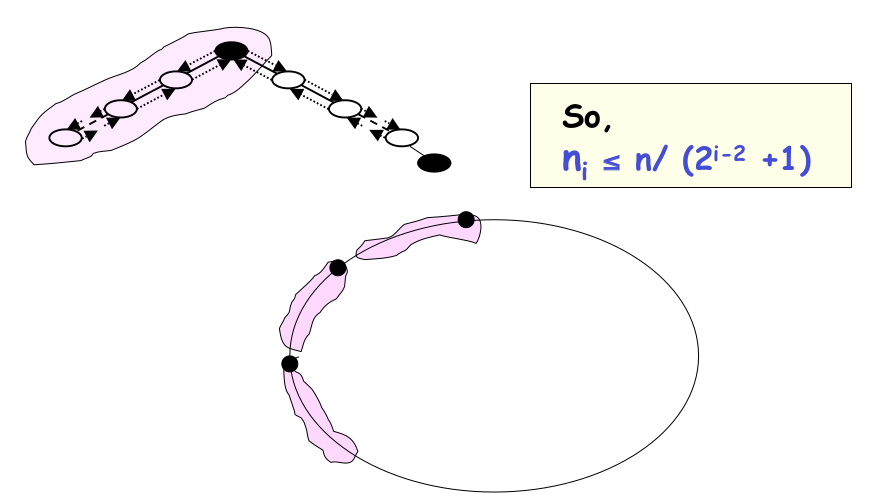
\includegraphics[width=0.8\textwidth]{images/stage_tecnique_msg.png}
            \caption{Nodi che sopravvivono allo stage $i$.
            \label{fig:stage_tecnique_msg}}
        \end{figure}
        
        Non ci può essere più di un sopravvissuto ogni $2^{i-2}$ nodi in quanto se ce ne fossero di più, per esempio $x$ e $y$, vorrebbe dire che $x$ ed $y$ si sono scambiati le etichette senza però che uno dei due venisse "sconfitto", e ciò implicherebbe che $id(x) < id(y) < id(x)$.

        Contiamo ora il numero di messaggi scambiati durante lo stage $i$. Abbiamo due tipologie di messaggi, quelli di tipo \texttt{Forth} e quelli di tipo \texttt{Back}. 
        \begin{description}
            \item[FORTH:] Ogni nodo candidato $x$ inoltra la sua etichetta ad \textbf{al più} $2 \cdot 2^{i-1} = 2^i$ nodi, per un totale di $n_i \cdot 2^i$
            \item[BACK:] Poiché nella fase $i$ sopravviveranno $n_{i+1}$ candidati, per ognuno verranno necessariamente trasmessi altri $2 \cdot 2^{i-1} = 2^i$ messaggi di feedback, per un totale di $n_{i+1} \cdot 2^i$.
        \end{description}
        Infine, rimangono i nodi \texttt{defeated}, che sono $n_i - n_{i+1}$. Questi riceveranno al massimo un messaggio di tipo \texttt{Back}, per un massimo di $2^{i-1}$ ulteriori messaggi, dunque, in totale, \textbf{al più} $2^{i-1} \cdot (n_i - n_{i+1})$ messaggi.
        
        Perciò, complessivamente, nella fase $i > 1$,
        \begin{align*}
            M[\texttt{stage}_i] 
            &= 2n_i2^{i_1} + 2n_{i+1}2^{i-1} + (n_i - n_{i+1})2^{i-1} = (3n_i + n_{i+1})2^{i-1} \\
            &\leq \left( 3 \bigg\lfloor \frac{n}{2^{i-2} + 1} \bigg\rfloor + \bigg\lfloor \frac{n}{2^{i-2} + 1} \bigg\rfloor \right)2^{i-1} \\
            &< \left( 3  \frac{n}{2^{i-2} + 1} + \frac{n}{2^{i-2} + 1} \right)2^{i-1} \\
            &< \left( 4  \frac{n}{2^{i-2}} \right)2^{i-1} \\
            &= 6n + n = 7n.
        \end{align*}
        
        \textbf{Osservazione.} Il numero di messaggi scambiati durante lo stage $1$ è diverso, poichè il caso peggiore si ha quando tutti i nodi sono iniziatori. In questo caso 
        \[
            n_2 \leq \frac{n}{2^0 + 1} = \frac{n}{2}
        \]
        I nodi che sopravvivono allo stage $1$ pagano individualmente 2 per \texttt{Forth} e 2 per \texttt{Back}, mentre i nodi che vengono sconfitti pagano individualmente 2 per \texttt{Forth} 1 per \texttt{Back}, in totale,
        \[
            M[\texttt{stage}_1] = 4n_2 + 3n - 3n - 3n_2 = n_2 + 3n < 4n.
        \]

        \textbf{Numero di stage.} Rimane solo da dimostrare che il numero di stage è $O(\log n)$. Sia $i^*$ lo stage in cui un nodo si dichiara leader, ossia quando riceverà da un lato il messaggio che ha inviato dal lato opposto, allora
        \[
            i^* = \min \{i \in \mathbb{N} : 2^{i-1} \geq n\} \iff i^* = O(\log n)
        \]
        Dunque il numero necessari di stage è $O(\log n)$, e poiché in ogni stage vengono scambiati al più $7n$ messaggi, la message complexity totale è
        \[
            M[\texttt{Stage Technique}] = \sum_{i=1}^{\log n} M[\texttt{stage}_i] + M[\texttt{stage}_1] = O(n \log n).
        \]
    \end{proof}
\end{teorema}

\newpage

\section{Mesh Architecture}
\begin{definizione}[Mesh]
    Una mesh è un grafo $\mathcal{M} = (V, E)$ dove:
    \begin{align*}
        V &= \{x_{i,j} : 1 \leq i \leq a,\ 1 \leq j \leq b\}, \quad |V| = n = ab \\
        E &= \{(x_{i,j}, x_{i+1,j}) : 1 \leq i < a, 1 \leq j \leq b\} \\
          &\quad \cup \{(x_{i,j}, x_{i,j+1}) : 1 \leq i \leq a, 1 \leq j < b\}, \quad |E| = m = 2ab - a - b.
    \end{align*}
    Una mesh è una griglia rettangolare di dimensioni $a \times b$ dove ogni nodo è collegato ai suoi vicini orizzontali e verticali.
\end{definizione}

\begin{figure}[htbp]
    \centering
    \begin{tikzpicture}
        \draw[thin, gray] (0,0) grid (8,4);

        \foreach \x in {0,...,8}
            \foreach \y in {0,...,4}
            {
                \filldraw[black] (\x,\y) circle (1pt);
            }
    \end{tikzpicture}
    \caption{Rappresentazione di una mesh $9 \times 5$.}
    \label{fig:mesh_9x5}
\end{figure}

In una mesh, possiamo distiguirere tre tipi di nodi (è una topologia \textbf{asimmetrica}):
\begin{itemize}
    \item \textbf{Corner nodes}: sono i nodi che si trovano agli angoli della griglia, e hanno grado 2.
    \item \textbf{Edge nodes}: sono i nodi che si trovano sui bordi della griglia, ma non agli angoli, e hanno grado 3 e ve ne sono $2(a+b)-4$.
    \item \textbf{Inner nodes}: sono i nodi che si trovano all'interno della griglia, e hanno grado 4 e ve ne sono $(a-2)(b-2)$.
\end{itemize}

\subsection{Protocollo}

Consideriamo il sottografo indotto dai nodi \textbf{corner} e dai nodi \textbf{edge}, che formano un anello. Eseguiamo su tale anello un protocollo di leader election per eleggere un leader tra i nodi \textbf{corner}. Essi saranno gli unici candidati, mentre i nodi \textbf{edge} avranno solo il ruolo di inoltro. Una volta eletto il leader, esso esegue una \texttt{broadcast} a tutta la rete, e ogni nodo si dichiara follower e termina localmente.

Il protocollo consiste di tre fasi:
\begin{enumerate}
    \item \textbf{Wake Up:} Ogni initiator ($k$) invia un messaggio di \texttt{wake-up} a tutti i suoi vicini. Ogni nodo non iniator che riceve il messagio di \texttt{wake-up}, lo invia agli altri vicini, in totale si scambiano
    \[
        M[\texttt{Wake Up}] = 3n + k = O(n).
    \]
    \item \textbf{Election on the Ring: } Poichè i nodi sanno di essere o edge o corner, possono eseguire un protocollo di leader election sull'anello formato da questi nodi. I nodi corner sono gli unici candidati, che inviano i propri id, mentre i nodi edge si limitano ad inoltrare i messaggi. Quindi, un nodo sa che ci sono esattamente 4 candidati, e una volta che ha ricevuto 4 id diversi può calcolare il minimo e dichiararsi o leader o follower e terminare localmente. La message complecity è:
    \[
        M[\texttt{Election on the Ring}] = O(a + b) = O(\sqrt{n}),
    \]
    poichè su ogni link dell'anello passano al più 4 messaggi, e l'anello è formato da $2(a+b)-4$ nodi.
    \item \textbf{Broadcast: } Il nodo leader esegue una \texttt{broadcast} a tutta la rete, e ogni nodo si dichiara follower e termina localmente. La message complexity è
    \[
        M[\texttt{Broadcast}] = O(n),
    \]
\end{enumerate}

\section{Randomized Algorithm}

Abbiamo visto che il problema della leader election non è risolvibile in modo deterministico in una rete in cui i nodi sono anonimi, ossia non esiste uno etichettamento univoco dei nodi. 

Consideriamo ora una anello $G = (V, E)$ di dimensione $n$, dove i nodi sono \textbf{anonimi}, e conoscono la topologia della rete e il numero di nodi $n$. In questo caso, è possibile risolvere il problema della leader election in modo \textbf{randomizzato}.

Ciascun nodo $x \in V$ sceglie, indipendentemente dagli altri nodi, la sua etichetta 
\[
    id(x) \xleftarrow{u.a.r.} [m] = \{1, \dots, m\},
\]
dove $m$ è un parametro che dipende da $n$ e che verrà scelto in modo opportuno, sperando che non esistano due nodi con la stessa etichetta. A questo punto, i nodi eseguono uno dei protocolli visti in precedenza (\texttt{All The Way, As Far, Stage Technique}) per eleggere un leader tra i nodi che hanno scelto l'etichetta minima.

Formalemente, il protocollo $\mathcal{RL}(G, n; m)$ è il seguente ($m$ è un parametro che dipende da $n$ e che verrà scelto in modo opportuno):
\begin{enumerate}
    \item \textbf{Wake-up:} Viene eseguito un protocollo di wake-up, in modo che tutti i nodi si attivino.
    \item \textbf{Random ID Generation:} Ogni nodo $x$ sceglie, indipendentemente dagli altri nodi, la sua etichetta $id(x)$ in modo uniforme a caso da $[m]$.
    \[
        id(x) \xleftarrow{u.a.r.} [m] = \{1, \dots, m\},
    \]
    \item \textbf{Leader Election:} I nodi eseguono uno dei protocolli \textit{deterministici} di leader election visti in precedenza, per eleggere un leader tra i nodi che hanno scelto l'etichetta minima.
\end{enumerate}

\subsection{Analisi}

Analizziamo ora la corretteza del protocollo, la message complexity ovviamente dipende da quale protocollo deterministico viene scelto, che abbiamo già analizzato, dunque ci concentriamo sulla probabilità di successo del protocollo.

Dobbiamo fare un'analisi probabilistica del protocollo. Innanzitutto definiamo lo spazio di probabilità, che è dato da tutte le possibili assegnazioni di etichette ai nodi, dunque
\[
    \Omega = [m]^n = \{(id(x_1), id(x_2), \ldots, id(x_n)) : id(x_i) \in [m],\ 1 \leq i \leq n\}.
\]

Osserviamo che un \textbf{evento sufficiente} (ma \textbf{non necessario}) affiché il protocollo termini \textbf{correttamente} è:

\[
    \mathcal{B} = "\text{non esistono due nodi differenti } u, w \in V,\ u \neq w:\ id(u) = id(w)"
\]

L'evento $\mathcal{B}$ è sufficiente perché se non esistono due nodi con la stessa etichetta, allora esiste un nodo con etichetta minima, e tale nodo sarà l'unico candidato, dunque verrà eletto leader, e tutti gli altri nodi si dichiareranno follower e termineranno localmente. Tuttavia, $\mathcal{B}$ non è necessario perché è possibile che esistano due nodi $u, v \in V$ con $u \neq v$ e $id(u) = id(v)$ ma che esista un nodo $w$ con $id(w) < id(u) = id(v)$, e quindi $w$ sarà l'unico candidato, e verrà eletto leader, e tutti gli altri nodi si dichiareranno follower e termineranno localmente.

Osserviamo che possiamo modellare il problema come un problema di \textbf{urne e palline} (\textit{Balls-into-Bins Process}), in cui abbiamo $n$ palline (i nodi) e $m$ urne (le possibili etichette), e ogni pallina viene lanciata in modo uniforme a caso in una delle $m$ urne. L'evento $\mathcal{B}$ si verifica se e solo se tutte le palline finiscono in urne diverse, ossia non esistono due palline che finiscono nella stessa urna.

Calcoliamo ora la probabilità che si verifichi l'evento $\mathcal{B}$. 
\[
    \mathcal{P}(\mathcal{B}) = 1 - \mathcal{P}(\overline{\mathcal{B}}) = 1 - \mathcal{P}("\text{esistono due nodi } u, w \in V,\ u \neq w:\ id(u) = id(w)")
\]

Per ogni $i \in [m]$, definiamo l'evento 
\[
    \overline{\mathcal{B}}_{i} = "\text{esistono due nodi } u, w \in V,\ u \neq w:\ id(u) = id(w) = i".
\]

Possiamo vedere l'evento $\overline{\mathcal{B}_i}$ come "almeno due palline finiscono nell'urna $i$", quindi,

Tale evento può essere modellato come l'unione di v.a. binamiali.

\begin{align*}
    \mathcal{P}(\overline{\mathcal{B}_i}) 
    &= \mathcal{P} \left( \bigcup_{k=2}^{n} \{ \text{esistono } k \text{ palline nell'urna } i \} \right) \\
    \text{unione di eventi disgiunti } &= \sum_{k=2}^{n} \mathcal{P} (\text{esistono } k \text{ palline nell'urna } i) \\
    &= \sum_{k=2}^{n} \binom{n}{k} \left( \frac{1}{m} \right)^k \left( 1 - \frac{1}{m} \right)^{n-k} \leq \sum_{k=2}^{n} \binom{n}{k} \left( \frac{1}{m} \right)^k \\
    \text{Stirling's approx } &\leq \sum_{k=2}^{n} \left( \frac{ne}{k} \cdot \frac{1}{m}\right)^k \leq O\left(\frac{n^2}{m^2}\right) + \sum_{k=3}^{n} \left( \frac{ne}{k} \cdot \frac{1}{m}\right)^k \\
    &\leq O\left(\frac{n^2}{m^2} + \frac{n^4}{m^3}\right)
\end{align*}

Adesso, possiamo calcolare la probabilità che si verifichi l'evento $\overline{\mathcal{B}}$, ossia che esistano due nodi con la stessa etichetta, utilizzando l'unione di eventi:
\begin{align*}
    \mathcal{P}(\overline{\mathcal{B}})
    &= \mathcal{P} \left( \bigcup_{i=1}^{m} \overline{\mathcal{B}_i} \right) \\
    \text{union bound } &\leq \sum_{i=1}^{m} \mathcal{P}(\overline{\mathcal{B}_i}) \\
    &\leq m \cdot O\left(\frac{n^2}{m^2} + \frac{n^4}{m^3}\right) = O\left(\frac{n^2}{m} + \frac{n^4}{m^2}\right)
\end{align*}

Ponendo ora $m = n^3$, avremo che tale probabilità sarà al più
\[
    \mathcal{P}(\overline{\mathcal{B}}) = O\left(\frac{n^2}{n^3} + \frac{n^4}{n^6}\right) \in O\left(\frac{1}{n}\right).
\]

Possiamo quindi concludere che per $m \geq n^3$, l'esecuzione del protocollo $\mathcal{RL}(G, n; m)$ porterà la rete in una configurazione finale accettabile con \textbf{alta probabilità (w.h.p.)} 
\[
    \mathcal{P}(\mathcal{B}) = 1 - O\left(\frac{1}{n}\right)
\]

\chapter{Graph Coloring}

\begin{definizione}[$\alpha$-coloring]
    Sia $G = (V, E)$ un grafo. Un $\alpha$-\textit{coloring} di $G$ è un'etichettamento dei vertici di $G$ tale che nessun coppia di vertici adiacenti condivida la stessa etichetta. Formalemnte, è una funzione
    \[
        c: V \to \{1, 2, \ldots, \alpha\}
    \]
    è un $\alpha$-coloring se per ogni $(u, v) \in E$, $c(u) \neq c(v)$.
\end{definizione}

Nel mondo centralizzato, questo è un problema NP-completo, ma in un contesto distribuito, possiamo trovare soluzioni efficienti con algoritmi che sfruttano la comunicazione tra i nodi.

\section{Deterministic Distributed Graph Coloring}

Ci troviamo in un contesto $\mathcal{LOCAL}$, ossia ad ogni nodo è assegnata un'etichetta univoca $id(v)$ che solo lui conosce, ogni nodo può comunicare solo con i suoi vicini in \textbf{round discreti e sincroni}. Ogni nodo può eseguire un numero di computazioni potenzialmente illimitato e può inviare messaggi distinti a ciascuno dei suoi vicini in ogni round, e tali messaggi arrivano entro la fine del round.

Consideriamo ora il problema del \textbf{coloring} restringendolo a grafi $\Delta$-regolari, ossia grafi in cui ogni nodo ha al più $\Delta$ vicini. L'obiettivo è trovare un $(\Delta + 1)$-coloring in modo distribuito, poiché è noto che $\Delta + 1$ colori sono sufficienti per colorare qualsiasi grafo con grado massimo $\Delta$. In particolare:

\begin{itemize}
    \item $P_{init}$: una configurazione iniziale che consiste in un $\alpha$-coloring con $\alpha > \Delta + 1$.
    $$C_{init}: V \to [1, \alpha], \quad \forall v \in V, \; C_{init}(v) \in [1, \alpha]$$
    \item $P_{final}$: una configurazione finale che consiste in un $(\Delta + 1)$-coloring.
    $$C_{final}: V \to [1, \Delta + 1], \quad \forall v \in V, \; C_{final}(v) \in [1, \Delta + 1]$$
    \item Restrizioni standard più modello $\mathcal{LOCAL}$: $R = R \cup \mathcal{LOCAL}$.
\end{itemize}

\subsection{Basic Color Reduction Procedure - BCP}

La \textbf{BCP} è una tecnica deterministica che permette di ridurre il numero di colori in $G$ da $\alpha$ a $\Delta + 1$ in $O(\alpha - (\Delta + 1))$ rounds. 

Ogni nodo $v$ esegue in parallelo i seguenti passi per ogni round:

\begin{enumerate}
    \item Trasmette il proprio colore $c(v)$ a tutti i vicini $u \in N(v)$ e riceve il colore $c(u)$ da ciascuno di essi.
    \item Seleziona un nuovo colore $c'(v)$ dall'insieme dei colori \emph{disponibili}, definito come:
    \[
        \mathcal{A}(v) = \{1, \dots, k\} \setminus \{c(u) \mid u \in N(v)\}
    \]
    \item Se $c'(v) \neq c(v)$, aggiorna il proprio colore: $c(v) \leftarrow c'(v)$.
\end{enumerate}

Il processo termina quando ogni nodo $v$ ha un colore distinto da quello di tutti i suoi vicini, ovvero quando la colorazione è \emph{propria}.

\begin{algorithm}
\caption{BCP}
\begin{algorithmic}[1]
\For{node $v \in V$}
    \For{phase $k = \alpha, \alpha-1, \dots, \Delta+2$}
        \State \textbf{send} $C(v)$ to $N(v)$
        \State \textbf{receive} $C(u)$ for all $u \in N(v)$
        \If{$C(v) = k$}
            \State choose $j \in \{1, \dots, k-1\} \setminus C(N(v))$
            \State $C(v) \leftarrow j$
        \EndIf
    \EndFor
\EndFor
\end{algorithmic}
\end{algorithm}

\begin{teorema}[Correttezza]
    Il protocollo BCP ritorna un $(\Delta + 1)$-coloring
    \[
        C_{final}: V \to [1, \Delta + 1]
    \]
    \begin{proof}
        Valgono i seguenti fatti:
        \begin{description}
            \item[FACT 1:] Poiché $k > \Delta + 1$ e poichè ad ogni round $k$, il nodo $v \in V:\ c(v) = k$ ha al più $\Delta$ vicini che possono avere $\Delta$ colori distinti, allora il nodo $v$ ha almeno un colore disponibile $j < k:\ j \in [1, k-1] \setminus C(N(v))$.
            
            Formalmente, poiché $|N(v)| \leq \Delta$ e $k > \Delta + 1$, abbiamo:
            \[
                |[k-1] \setminus C(N(v))| = |[k-1]| - |C(N(v))| > \Delta - \Delta = 0 \quad (\geq 1)
            \]
            Quindi, esiste almeno un colore $j$ che non è utilizzato dai vicini di $v$.
            \item[FACT 2:] Al termine di ogni round $k > \Delta + 1$, la colorazione $C_k: V \to [1, k-1]$ è legale. Poiché si parte da una colorazione legale, e ad ogni round solo i nodi con colore $k$ cambiano il loro colore (che per definizione di colorazione legale, non sono vicini), e ogni nodo $v$ che cambia colore sceglie un nuovo colore $j$ che è disponibile (non utilizzato dai vicini), allora la colorazione rimane legale.
        \end{description}
    \end{proof}
\end{teorema}

\begin{teorema}[Time Complexity \& Message Complexity]
    Vale il seguente:
    \begin{itemize}
        \item $T[BCP] = O(\alpha - (\Delta + 1))$. Se $\alpha \in O(n)$, allora $T[BCP] = O(n - \Delta)$. Inoltre, il caso peggiore si verifica quando $\Delta = O(1)$.
        \item $M[BCP] = O(m \cdot (\alpha - \Delta))$ oppure se $\alpha \in O(n)$, allora $M[BCP] = O(m \cdot (n - \Delta))$.
    \end{itemize}
\end{teorema}

\subsection{Khun-Wattenhofen Procedure}

Vediamo ora una procedura che permette di velocizzare la riduzione dei colori da $\alpha > 2(\Delta + 1)$ a $\Delta + 1$ in tempo $O(\Delta \log\frac{\alpha}{\Delta})$ invece che $O(\alpha - (\Delta + 1))$.

L'idea è di eseguire BCP in modo parallelo, di seguito i passi:

\begin{enumerate}
    \item Partizionare l'insieme dei nodi $V$ in $k = \left\lceil \frac{\alpha}{\Delta + 1} \right\rceil$ sottoinsiemi disgiunti $V_1, V_2, \dots, V_k$ tali che
    \[
        V_i = \{v \in V \mid C(v) \in [(i-1)(\Delta + 1) + 1, i(\Delta + 1)]\}
    \]
    \item Eseguire BCP in parallelo sul grafo indotto $G_{i, (i + 1)} = (V_i \cup V_{i+1}, E)$.
    Qui si distinguono due casi:
    \begin{itemize}
        \item   Se $k$ è pari, allora eseguiamo BCP in parallelo sui grafi indotti $G_{i, i+1}$ per $i = 1, 3, \dots, k-1$, dove la colorazione indotta da $C_{init}$ è 
        \[
            F_{i, i+1}: V_i \cup V_{i+1} \to [(i-1)(\Delta + 1) + 1, (i + 1)(\Delta + 1)]
        \]
        \item   Se $k$ è dispari, allora eseguiamo BCP in parallelo sui grafi indotti $G_{i, i+1}$ per $i = 1, 3, \dots, k-4$ e su $G_{k-2, k-1, k}$, dove la colorazione indotta da $C_{init}$ è
        \[
            F_{i, i+1}: V_i \cup V_{i+1} \to [(i-1)(\Delta + 1) + 1, (i + 1)(\Delta + 1)]
        \]
         e
        \[
            F_{k-2, k-1, k}: V_{k-2} \cup V_{k-1} \cup V_k \to [(k-3)(\Delta + 1) + 1, \alpha]
        \]
    \end{itemize}
    
    imponendo il numero di rounds $k = i(\Delta + 1) \dots (i+1)(\Delta + 1)$. 
    
    Questo grafo ammette una colorazione con al più $2(\Delta + 1)$ colori, quindi BCP può essere eseguito in $O(\Delta)$ rounds per ridurre i colori a $\Delta + 1$.
    \item Ripetere il passo 1 e 2 fino a quando il numero di colori è ridotto a $\Delta + 1$.
\end{enumerate}

\textbf{Esempio}

Consideriamo un grafo con $\Delta = 2$ e $\alpha = 11$. In questo caso, $k = \lceil \frac{11}{3} \rceil = 4$, quindi partizioniamo i nodi in quattro sottoinsiemi $V_1, V_2, V_3, V_4$ come nella figura \autoref{fig:khunProcedure}. Successivamente, eseguiamo BCP in parallelo sui grafi indotti $G_{12}. G_{34}$.

Consideriamo $\texttt{BCP}(G_{12})$. Allora le fasi vanno da $k = 3, \dots, 6$. L'\texttt{if c(v) == k} verrà eseguito sarà per $c(v) \in {3, 5, 6}$.
\begin{itemize}
    \item Se $c(v) = 3$, allora $v$ sceglierà un nuovo colore $j \in \{1, 2\} \setminus \{2\} = \{1\}$.
    \item Se $c(v) = 5$, allora $v$ sceglierà un nuovo colore $j \in \{1, 2, 3, 4\} \setminus \{6\} = \{1, 2, 3, 4\}$.
    \item Se $c(v) = 6$, allora $v$ sceglierà un nuovo colore $j \in \{1, 2, 3, 4, 5\} \setminus \{5\} = \{1, 2, 3, 4\}$.
\end{itemize}

In questo modo, come possiamo osservare, il numero di colori viene ridotto almeno di uno ad ogni round.

\begin{figure}[h]
    \centering
    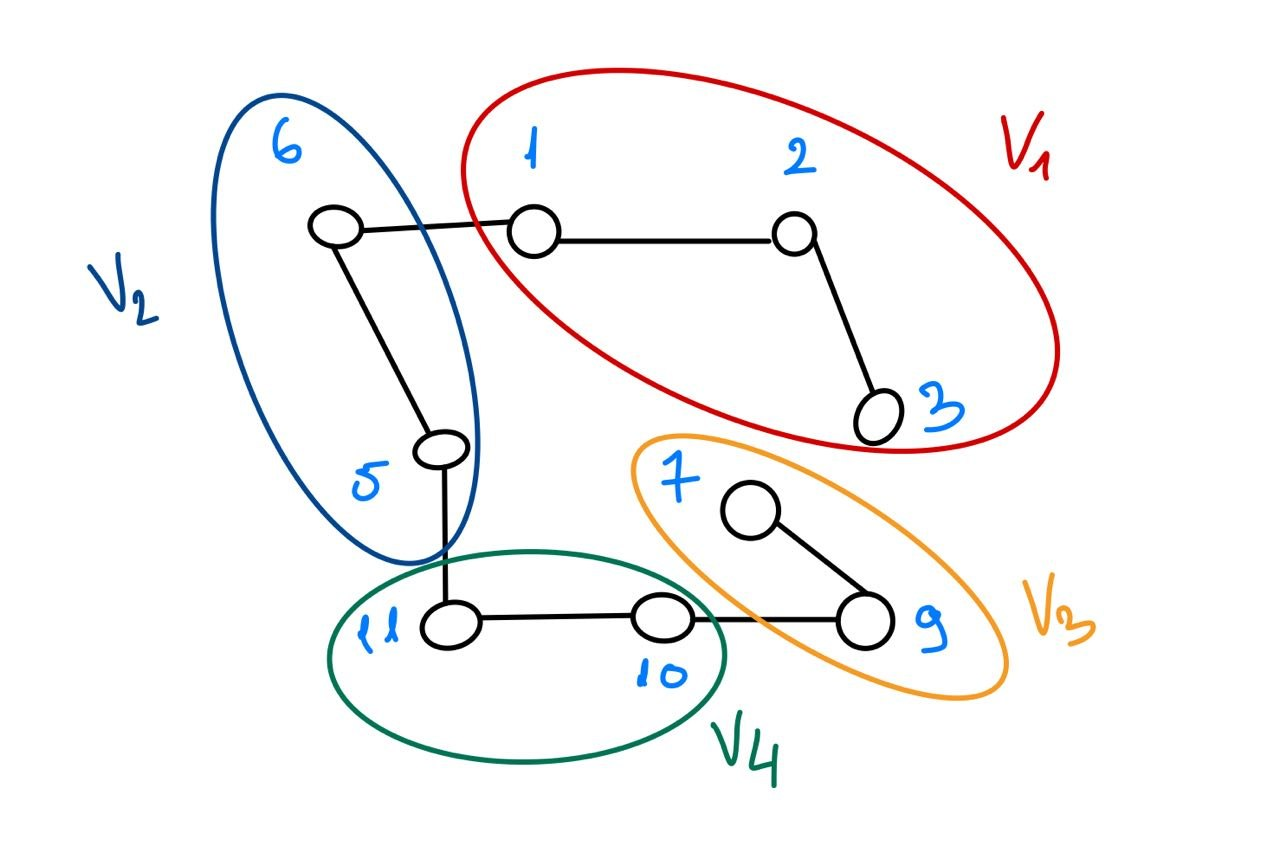
\includegraphics[width=0.4\textwidth]{images/khunProcedure.jpg}
    \caption{Esempio di partizione del grafo.}
\end{figure}\label{fig:khunProcedure}

Dopo un'iterazione di questa procudera parallela, il numero di colori sarà ridotto a $\alpha' = \lceil \frac{\alpha}{2} \rceil$. Cosi facendo, in tempo $O(\Delta)$ abbiamo \textbf{dimezzato} i colori della colorazione iniziale. Ripetendo, ogni $O(\Delta)$ si dimezza il numero di sottoinsiemi, e dopo $\log(\frac{\alpha}{\Delta})$ iterazioni avremo ridotto il numero di colori a $\Delta + 1$. In totale, la complessità temporale è $O(\Delta \log\frac{\alpha}{\Delta})$.

\section{Randomized Distributed Graph Coloring}

Un approccio probabilistico molto usato per risolvere questa tipologia di problemi distribuiti (non solo il \texttt{Graph Coloring}, ma per esempio anche il \texttt{Maximal Independent Set}) è il seguente: il protocollo procede per \textbf{fasi}, dove in ciascuna di esse ogni nodo sceglie casualmente un valore da un insieme appropriato di colori. In base al colore scelto, e a quello scelto dai propri vicini, ogni nodo deve prendere la decisione finale di adottare il colore scelto e terminare il protocollo, oppure di continuare alla fase successiva.

Osservare che tutti i nodi che prendono una decisione finale formano un sottoinsieme della soluzione finale. Perciò basta rimuovere i nodi che hanno terminato il protocollo, e procedere alla stessa maniera però sul grafo residuo. Un requisito importante che una soluzione parziale deve necessariamente avere è che essa non solo deve essere corretta nel relativo sottoinsieme di vertici, ma anche rispetto all'unione di tutti i sottoinsiemi rimossi nelle fasi successive. Il protocollo termina quando verranno rimossi tutti i nodi dal grafo, ovvero quando tutti i nodi avranno scelto definitivamente il proprio colore.

\subsection{Rand-2$\Delta$}

Definiamo formalemente il problema del \texttt{Rand-$2\Delta$-Coloring}:
\begin{itemize}
    \item $P_{init}$: Una colorazione iniziale dei nodi $C_{init}: V \to [\alpha]$ con $\alpha > 2\Delta$.
    \item $P_{final}$: Una colorazione finale dei nodi $C_{final}: V \to [2\Delta]$.
    \item Restrizioni standard più modello $\mathcal{LOCAL}$: $R = R \cup \mathcal{LOCAL}$.
\end{itemize}

Entriamo ora nel merito del protocollo \texttt{Rand-$2\Delta$} che calcola in maniera distribuita una $2\Delta$ colorazione di un grafo $G$ in accordo all'approccio precedente, dove $\Delta$ è il grado massimo di $G$. Ad ogni fase, ogni nodo $v$ campiona \textit{u.a.r.} un colore $c(v)$ dall'insieme $[2\Delta]=\{1,2,\ldots,2\Delta\}$. Indichiamo con $F_v$ l'insieme dei colori scelti definitivamente dai vicini di $v$, e con $T_v$ l'insieme dei colori scelti (temporaneamente) dai vicini di $v$ nel corrente round. Se $c(v) \notin F_v \cup T_v$, allora $c(v)$ diventa il colore definitivo di $v$, e in tal caso il nodo termina il protocollo. Altrimenti $v$ scarta $c(v)$ e continua alla fase successiva.

\begin{algorithm}
\caption{Procedure \textsc{Rand-2Delta}($G$)}
\begin{algorithmic}[1]

\State An algorithm for each vertex $v \in V$.
\State Initially $T_v = \emptyset$, $F_v = \emptyset$, for each $v \in V$.
\State \textit{$T_v$ is the set of temporary colors selected by neighbors of $v$.}
\State \textit{$F_v$ is the set of final colors selected by neighbors of $v$.}

\For{each round}
    \State $T_v = \emptyset$
    \State $c(v) :=$ draw a color from $[2\Delta]$ u.a.r., independently of other vertices
    \State $\texttt{send}(c(v)) \to N(v)$
    \For{each received color $c(u)$ from a neighbor $u$}
        \State $T_v := T_v \cup \{c(u)\}$
    \EndFor
    \If{$c(v) \notin T_v \cup F_v$}
        \State $\texttt{send}(\texttt{final} \; c(v)) \to N(v)$
        \State select $c(v)$ as the final color $\varphi_v$ of $v$ and \textbf{terminate}
    \Else
        \For{each received message $\texttt{final} \; c(u)$ from a neighbor $u$}
            \State $F_v := F_v \cup \{c(u)\}$
        \EndFor
        \State discard $c(v)$ and continue to the next round
    \EndIf
\EndFor

\end{algorithmic}
\end{algorithm}

\newpage

\begin{teorema}[Correttezza]
    Se tutti i nodi terminano, allora il protocollo \texttt{Rand-$2\Delta$} calcola una $2\Delta$-colorazione del grafo $G$ in input.
    \begin{proof}
        Sappiamo con certezza che la colorazione finale $\varphi$ è una $2\Delta$-colorazione di $G$, perché per costruzione tutti i colori scelti dai nodi sono nell'insieme $[2\Delta]$, perciò serve solamente dimostrare che la colorazione $\varphi$ sia legale.

        Consideriamo due nodi adiacenti $u$ e $v$, e supponiamo per assurdo che alla fine del protocollo, $\varphi(u) = \varphi(v)$. Certamente i due nodi non possono aver terminato il protocollo nello stesso round, in quanto sarebbe accaduto che $c(u) \in T_u$ e $c(v) \in T_v$ (il controllo qui dentro non sarebbe false, vedi \texttt{riga 12}). Allora siano $i$ e $j$ i rounf in cui i nodi $u$ e $v$ hanno terminato ed assumiamo senza perdita di generalità che $i < j$. Allora dal round $i$ in poi, il colore definitivo $\varphi(u)$ sarà presente in $F_v$. Perciò, per costruzione dell'algoritmo, il colore definitivo $\varphi(v)$ sarà scelto al tempo $j$ in modo tale che $\varphi(v) \notin F_v$ (la condizione a \texttt{riga 12} sarà true), e quindi $\varphi(v) \neq \varphi(u)$, il che è una contraddizione.
    \end{proof}
\end{teorema}

\begin{teorema}[Time Complexity]
    Durante l'esecuzione del protocollo \texttt{Rand-$2\Delta$} tutti i nodi terminano la loro esecuzione entro $O(\log n)$ rounds con alta probabilità, $1 - \frac{1}{n^c}$ per una costante $c > 0$.
    \begin{proof}
        Consideriamo un qualisiasi nodo $v \in V$ e calcoliamo la probabilità che $v$ termini nel round $i$ condizionato al fatto che non ha terminato prima, per ogni $i \geq 1$.
        
        Osserviamo che $|T_v \Cup F_v| \leq \Delta$ perché ogni vicino di $v$ contribuisce con al più un colore a questo insieme, e inoltre $|N(v)| \leq \Delta$. Di conseguenza $v$ ha a disposizione \textbf{almeno} $\Delta$ colori valori per la colorazione finale nell'insieme $[2\Delta] \setminus (T_v \cup F_v)$. Perciò la probabilità che $v$ scelga un colore valido finale sarà almeno
        \[
            P(c(v) \notin T_v \cup F_v) = \frac{|[2\Delta] \setminus (T_v \cup F_v)|}{|[2\Delta]|} \geq \frac{\Delta}{2\Delta} = \frac{1}{2}
        \]

        Quindi, assumento che $v$ non termina \textbf{prima} del round $i$, la probabilità che termini al round $i$ è almeno $\frac{1}{2}$ \textbf{indipendentemente} dagli altri nodi.
        \[
            P(v \text{ termina al tempo } i \mid v \text{ non termina prima di } i) \geq \frac{1}{2}
        \]

        Viceversa, la probabilità che un dato nodo $v$ \textbf{non} termina entro il passo $i$ sarà al più $2^{-i}$. Facendo \textit{union bound} possiamo calcolare la probabilità che esista un nodo $v$ che entro il tempo $i$ non ha ancora finito come segue:
        \[
            P(\exists v \in V: v \text{ non termina entro } i) \leq \sum_{v \in V} P(v \text{ non termina entro }i) \leq n \cdot 2^{-i}
        \]

        Per $i = c \log n$ con $c > 0$, otteniamo che la probabilità che esista un nodo $v$ che non ha terminato entro il tempo $i$ è al più $\frac{1}{n^c}$, e di conseguenza la probabilità che tutti i nodi terminino entro il tempo $i$ è almeno $1 - \frac{1}{n^c}$. Quindi, con alta probabilità, tutti i nodi terminano entro $O(\log n)$ rounds.
    \end{proof}
\end{teorema}

\subsection{Rand-$\Delta$+}

Il protocollo \texttt{Rand-$\Delta$+} è una variante del protocollo \texttt{Rand-$2\Delta$} che permette di ridurre il numero di colori finali da $2\Delta$ a $\Delta + 1$. 

L'idea è quella che ogni nodo ad ogni iterazione deve prima partecipare ad una lotteria, e solo se vince la lotteria, allora può campionare un colore da $[\Delta + 1]$ e tentare di terminare. Nello specifico, le modifiche effettuate al protocollo iniziale sono le seguenti:
\begin{itemize}
    \item Ogni nodo $v \in V$ che partecipa alla fase $i$ sceglie \textit{u.a.r.} un bit $c(v) \in \{0,1\}$; se $c(v) = 0$, allora $v$ non partecipa alla scelta di un colore e viene direttamente fatto passare alla fase successiva.
    \item Ogni nodo $v \in V$ che partecipa alla fase $i$ (ossia quelli che hanno scelto $c(v) = 1$) sceglie \textit{u.a.r.} un colore $col(v)$ dalla palette $[\Delta + 1] \setminus F_v$. A questo punto il protocollo esegue come \texttt{Rand-$2\Delta$}.
\end{itemize}

\begin{teorema}[Correttezza]
    Se tutti i nodi terminano, allora il protocollo \texttt{Rand-$\Delta$+} calcola una $(\Delta + 1)$-colorazione del grafo $G$ in input.
\end{teorema}

\begin{teorema}[Time Complexity]
    Durante l'esecuzione del protocollo \texttt{Rand-$\Delta$+} tutti i nodi terminano la loro esecuzione entro $O(\log n)$ rounds con alta probabilità, $1 - \frac{1}{n^c}$ per una costante $c > 0$.
\end{teorema}

\include{maximal_ind_set}
\chapter{Averaging Protocol}

Consideriamo una rete modellata come un grafo connesso e non bipartito $G = (V, E)$. Ci troviamo sotto le restrizioni 
\[
    R = \{\texttt{TR, CN, BL, SYNC, LOCAL}\} 
\]
Ogni nodo $v \in V$ possiede un valore, diciamo $x(v) \in \mathbb{R}^+$ e localmente deve calcolare la media globale $\mu$ di tutti i valori posseduti da ciascun nodo
\[
    \mu=\frac{1}{|V|}\sum_{v\in V} x(v).
\]
Si richiede quindi una computazione distribuita della media: al termine, ogni nodo deve aver eseguito il calcolo di \(\mu\) a partire dalle sole informazioni scambiate nel protocollo.

Possiamo quindi modellare il problema con la tripla $\langle P_{init}, P_{final}, R\rangle$, dove

\begin{itemize}
    \item $P_{init}:$ la configurazione iniziale di ciascun nodo è $x^{(0)}(v)$. Se consideriamo tutti i valori inizali, allora possiamo definire un vettore $\mathbf{x} = \langle x^{(0)}(1), \dots, x^{(0)}(n)\rangle^T$
    \item $P_{final}$ la configurazione finale di ciascun nodo è $x^{(t)}:\ |x^{(t)} - x^{(t-1)}| \leq \epsilon$.
\end{itemize}

Definiamo quindi il protocollo \texttt{AVG} come segue:
\begin{enumerate}
    \item Al round $t = 0$, ogni nodo $v \in V$ possiede un valore iniziale $x^{(0)}(v) \in \mathbb{R}$
    \item Ad ogni round $t \geq 1$, ogni nodo $v \in V$ aggiora il suo valore $x^{(t)}(v)$ con la \textbf{media dei valori posseduti dai suoi vicini} al termine del round precedente $t - 1$, ossia
    \[
        x^{(t)}(v) = \frac{1}{\delta(v)} \sum_{u \in N(v)} x^{(t-1)}(u)
    \]
    \item Se $x^{(t)}:\ |x^{(t)} - x^{(t-1)}| \leq \epsilon$ allora \textbf{return} $x^{(t)}$ e \textbf{stop}.
\end{enumerate}

Definiamo $\forall v \in V$ il suo grado come $\delta(v) = |N(v)|$ (compreso se stesso). Diremo inoltre che il grafo è $\delta$\texttt{-regular} se $\delta(v) = \delta\ \forall v \in V$.

\section{Analisi del protocolo \texttt{AVG} per grafi $\delta$\texttt{-regular} e connessi}

\begin{teorema}[Message Complexity]
    La message complexity ad ogni round del protocollo \texttt{AVG} è $\theta(m)$.
    \begin{proof}
        Consideriamo il nodo $v \in V$ e contiamo il numero di messaggi che invia per round. Ad ogni rount $t,\ v$ invia $x^{(t)}(v)$ a ciascuno dei suoi $\delta(v)$ vicini, quindi in totale, abbiamo che il numero di messaggi scambiati ad ogni round è:
        \[
            M[\texttt{AVG}]_t = \sum_{v \in V} \delta(v) = \sum_{v \in V} \delta(v) = 2m \in \theta(m)
        \]
    \end{proof}
\end{teorema}

Vogliamo ora dimostrare che questo protocollo, converge ad un certo valore $\mu$ che è esattamente la media globale, e inoltre vogliamo determinare il tempo di convergenza.

\subsection{Convergenza}

\begin{teorema}[Convergenza]\label{teo:convergenza}
    Se il grafo $G = (V, E)$ è connesso, non bipartito e $\delta\texttt{-regular}$, allora il protocollo \texttt{AVG} converge in norma $L_2$ ad una configurazione stabile nella quale ogni nodo ha come valore 
    \[
        x(v) = \frac{1}{n}\sum_{v \in V} x^{(0)}(v)
    \]
    ossia, \textbf{converge} alla \textbf{media globale}.
\end{teorema}

La dimostrazione di questo teorema si articola in diverse fasi. In primo luogo, stabiliremo la convergenza nel caso più generale di un grafo non $\delta\texttt{-regular}$, per poi applicare l'ipotesi di regolarità.

Inoltre, per dimostrare questo teorema, faremo uso dell'algebra lineare e della teoria spettrale.

\begin{definizione}[Norma $L_p$]
    Sia $\mathbf{x} \in \mathbb{R}^n$, per ogni $p \in \mathbb{N}$ fissato, definiamo la norma $L_p$ come
    \[
        \norm{\mathbf{x}}_p = \left( \sum_{i = 1}^{n} |x_j|^p \right)^{1/p}
    \]
\end{definizione}

\begin{definizione}[Norma $L_\infty$]
    Sia $\mathbf{x} \in \mathbb{R}^n$, definiamo la norma $L_\infty$ come
    \[
        \norm{\mathbf{x}}_\infty = \max \{ |x_j|: j \in [n] \}
    \]
\end{definizione}

\begin{lemma}
    Per ogni vettore $\mathbf{x} \in \mathbb{R}^n$, vale che:
    \[
        \norm{\mathbf{x}}_\infty \leq \norm{\mathbf{x}}_2 \leq \norm{\mathbf{x}}_1 \leq \sqrt{n}\norm{\mathbf{x}}_2 \leq n\norm{\mathbf{x}}_\infty
    \]
\end{lemma}

\begin{definizione}[Base Ortonormale]
    Sia $V$ uno spazio vettoriale di dimensione finita sul campo $K$, nel quale sia definito il prodotto scalare. Una base ortonormale per $V$ è una base composta dai vettori $\langle \mathbf{u}_1, \dots, \mathbf{u}_n \rangle$ tale che:
    \begin{itemize}
        \item \textbf{Vettori mutualmente ortogonali:} $\langle \mathbf{u}_i, \mathbf{u}_j \rangle = 0, \quad \forall i \neq j$
        \item \textbf{Norma uguale a 1:} $\norm{\mathbf{u}_i}_2 = 1$
    \end{itemize}
\end{definizione}
Se $B = \langle \mathbf{u}_1, \dots, \mathbf{u}_n \rangle$ è ortonormale, allora
\[    
    \mathbf{x} = \sum_{\mathbf{u}_i \in B} \langle \mathbf{x}, \mathbf{u}_i \rangle \mathbf{u}_i
\]

Infine, definiamo la matrice di adiacenza $A,\ n \times n$ del grafo $G$ ponendo $A(i, j) = 1 \iff (i, j) \in E$. Definiamo inoltre la matrice diagonale $D^{-1},\ n \times n$ ponendo $D^{-1}(i, i) =  \frac{1}{\delta(i)}\ \forall i \in V$ e nelle altre entrate 0.

\begin{lemma}
    Per ogni round $t \geq 1$, la configurazione del sistema al round $t$ soddisfa la seguente equazione:
    \begin{equation}\label{eq:1}
        \mathbf{x}^{(0)} := \mathbf{x} \qquad \mathbf{x}^{(t+1)} := (D^{-1}A)\mathbf{x}^{(t)} = D^{-1} (A\mathbf{x}^t) 
    \end{equation}
    Più precisamente, se definiamo la matrice $P := D^{-1}A$ la \textbf{matrice di transizione} del grafo $G$, allora
    \begin{equation}\label{eq:2}
        \mathbf{x}^{(0)} := \mathbf{x} \qquad \mathbf{x}^{(t+1)} := P\mathbf{x}^{(t)} = PP\mathbf{x}^{(t-1)} = \dots = P^t\mathbf{x} \quad \text{Power Method}
    \end{equation}
    Questa equazione ci sta modellando un sistema dinamico lineare, in cui la configurazione al round $t + 1$ è ottenuta moltiplicando la matrice $P$ per la configurazione al round $t$.
    \begin{proof}
        Per ogni $i \in V$, possiamo scrivere la componente $i$-esima del vettore $\mathbf{x^{(t+1)}}$ come
        \[
            x^{(t+1)}(i) = \frac{1}{\delta(i)} \sum_{j = 1}^{n} A(i, j)x^{(t)}(j) = \frac{1}{\delta(i)} \sum_{j \in N(i)}x^{(t)}(j)
        \]
    \end{proof}
\end{lemma}

\textbf{Osservazione:} La matrice $P$ è \textbf{diagonalizzabile}, poichè è una matrice \textit{simile} ad una simmetrica.

\begin{definizione}[Matrici Simili]
    Due matrici $A, B,\ n \times n$ si dicono simili se esiste una matrice invertibile $M$ con la proprietà che $B = M^{-1}AM$
\end{definizione}

\begin{teorema}
    Se $A$ e $B$ sono matrici simili, allora:
    \begin{enumerate}
        \item $\det A = \det B$;
        \item $c_A(x) = c_B(x)$;
        \item $A$ e $B$ hanno gli stessi autovalori.
    \end{enumerate}
\end{teorema}

\begin{lemma}
    $P$ è una matrice simile alla matrice simmetrica $\tilde{P}$:
    \[
        \tilde{P} = D^{1/2}PD^{-1/2} = D^{1/2}\left(D^{-1}A\right)D^{-1/2} = D^{-1/2}AD^{-1/2}.
    \]
    Inoltre, $\tilde{P}$ è simmetrica, poiché:
    \[
        \tilde{P}^T = \left(D^{-1/2}AD^{-1/2}\right)^T = D^{-1/2}A^TD^{-1/2} = D^{-1/2}AD^{-1/2} = \tilde{P}.
    \]
\end{lemma}

Poichè $\tilde{P}$ è simmetrica, per il \textbf{Teorema Spettrale} ammette una base ortonormale di autovettori $\{\tilde{u}_1, \ldots, \tilde{u}_n\}$ con autovalori reali. Inoltre, poichè $P$ e $\tilde{P}$ sono simili, hanno gli stessi autovalori.

\textbf{Trasformazione degli autovettori.} Se $\tilde{u}$ è autovettore di $\tilde{P}$ con autovalore $\lambda$, ovvero $\tilde{P}\tilde{u} = \lambda\tilde{u}$, sostituendo la definizione di $\tilde{P}$:
\[
    D^{1/2}PD^{-1/2}\tilde{u} = \lambda\tilde{u}.
\]
Moltiplicando ambo i membri a sinistra per $D^{-1/2}$:
\[
    PD^{-1/2}\tilde{u} = \lambda D^{-1/2}\tilde{u}.
\]
Quindi $u = D^{-1/2}\tilde{u}$ è autovettore di $P$ con lo stesso autovalore $\lambda$. Poichè la trasformazione $\tilde{u} \mapsto D^{-1/2}\tilde{u}$ è invertibile (in quanto $D^{-1/2}$ è invertibile), gli $n$ autovettori $\{u_1, \ldots, u_n\}$ così ottenuti formano una \textbf{base di autovettori per} $P$, che risulta quindi diagonalizzabile.

\textbf{Osservazione:} La matrice $P$ è \textbf{stocastica}, ossia rispetta le seguenti proprietà:
\begin{itemize}
    \item \textbf{Non negatività degli elementi:}
    \[
        \forall i,j \in [n],\ P_{i,j} \geq 0
    \]
    \item \textbf{Somma unitaria per ogni riga:}
    \[
        \forall i \in [n],\ \sum_{j = 1}^{n} P_{ij} = 1
    \]
\end{itemize}
Inoltre, se $G$ è anche \textbf{regolare}, allora la matrice $P$ è \textbf{doppiamente stocastica}, $(P = P^T)$ ossia vale anche la \textbf{somma unitaria per ogni colonna:}
\[
    \forall j \in [n],\ \sum_{i = 1}^{n} P_{ij} = 1
\]

Applicando la teoria spettrale (decomposizione spettrale), possiamo individuare gli autovalori di $P$ e le loro proprietà.

Vogliamo studiare la convergenza del sistema in norma $L_2$.

\begin{lemma}
    Assumendo che $G$ è connesso e non bipartito e poichè la matrice $P$ è positiva a valori reali, ammette quindi $n$ autovalori $\lambda_1, \lambda_2, \dots, \lambda_n$ tali per cui $|\lambda_i| \leq 1,\ \forall i \in [n]$ e inoltre si ha un ordinamento di tali autovalori in senso non decrescente
    \[
        \langle \lambda_1 = 1, \lambda_2 < 1, \dots, \lambda_n \rangle
    \]
\end{lemma}

Ora, possiamo scrivere il vettore $\mathbf{x}$ come combinazione lineare della base formata dagli \textbf{autovettori} di $P$. Sia $\langle \mathbf{u}_1, \mathbf{u}_2, \dots, \mathbf{u}_n \rangle$ tale base, allora 
\[
    \mathbf{x} = \alpha_1\mathbf{u}_1 + \alpha_2\mathbf{u}_2 + \dots + \alpha_n\mathbf{u}_n
\]
e sostituendo nell'\autoref{eq:2}, otteniamo
\begin{equation}\label{eq:decomp-pt}
\begin{aligned}
    \mathbf{x}^{(t+1)}
    &= P^t \mathbf{x}
    = P^t\left(\alpha_1\mathbf{u}_1 + \alpha_2\mathbf{u}_2 + \dots + \alpha_n\mathbf{u}_n\right) \\
    &= \alpha_1 P^t\mathbf{u}_1 + \alpha_2 P^t\mathbf{u}_2 + \dots + \alpha_n P^t\mathbf{u}_n \\
    &= \alpha_1 \lambda_1^t \mathbf{u}_1 + \alpha_2 \lambda_2^t \mathbf{u}_2 + \dots + \alpha_n \lambda_n^t \mathbf{u}_n \\
    &= \alpha_1 \mathbf{u}_1 + \sum_{i=2}^{n} \alpha_i \lambda_i^t \mathbf{u}_i.
\end{aligned}
\end{equation}

\textbf{Osservazione:} Esistono autovettori con moltiplicità maggiore di 1, quindi è possibile che $\lambda_2 = \lambda_3 = \dots = \lambda_k$ per qualche $k > 2$. In questo caso, possiamo semplicemente raggruppare tali autovettori in un unico autovettore con autovalore $\lambda_2$.

Osserviamo quindi che per $t \to \infty$, siccome $|\lambda_i| < 1,\ \forall i > 1$, allora 
\[
    \sum_{i=2}^{n} \alpha_i \lambda_i^t \mathbf{u}_i \xrightarrow[t \to \infty]{} \mathbf{0}.
\]
in \textbf{norma}. 
Quindi, applicando un analisi spettrale della matrice di transizione $P$ del grafo, sotto certe condizioni abbiamo che il sistema converge ad uno stato stazionario $\alpha_1\mathbf{u}_1$.

Se sfruttiamo l'ipotesi di $\delta$\texttt{-regular} del grafo $G$ e quindi che la matrice $P$ è simmetrica, allora la base formata dagli autovettori $\langle \mathbf{u}_1, \mathbf{u}_2, \dots, \mathbf{u}_n \rangle$ è \textbf{ortonormale}, ossia i vettori $\mathbf{u}_i$ sono \textit{mutualmente} ortogonali avente norma $\norm{\mathbf{u}_i}_2 = 1$.

\begin{lemma}
    A partire da una qualsiasi configurazione iniziale $\mathbf{x}$, il sistema converge (in qualsiasi norma) a 
    \begin{equation}\label{eq:convergence}
        \mathbf{x}^{(t)} \to \alpha_1\mathbf{u}_1
    \end{equation}
\end{lemma}

Ci domandiamo ora chi sono $\alpha_1$ e $\mathbf{u}_1$. Per definizione di autovettore con autovalore $\lambda = 1$, abbiamo che $P \mathbf{u}_1 = \lambda \mathbf{u}_1 = \mathbf{u}_1$,
\[
\mathbf{u}_1 = P\,\mathbf{u}_1 =
\begin{bmatrix}
\frac{1}{\delta_1} & 0 & \cdots & \frac{1}{\delta_1} & 0 & \cdots & \frac{1}{\delta_1} \\
0 & \frac{1}{\delta_2} & \cdots & \frac{1}{\delta_2} & 0 & \cdots & 0 \\
\vdots & \vdots & \ddots & \vdots & \vdots & \ddots & \vdots \\
0 & 0 & \cdots & \frac{1}{\delta_i} & \cdots & \frac{1}{\delta_i} & 0 \\
0 & 0 & \cdots & \frac{1}{\delta_n} & \cdots & 0 & \frac{1}{\delta_n}
\end{bmatrix}
\begin{bmatrix}
u_1(1) \\
u_1(2) \\
\vdots \\
u_1(i) \\
\vdots \\
u_1(n)
\end{bmatrix}.
\]

Poiché a noi ci interessa la massa di $\mathbf{x}$ (ossia $\sum_{j \in V} x(j)$), possiamo considerare un qualsiasi autovettore $\mathbf{v}_1$ relativo a $\lambda = 1$ e lo possiamo normalizzare (ottenere un nuovo autovettore di norma 1) $\mathbf{u}_1$ nel seguente modo:
\[
    \mathbf{u}_1 = \frac{\mathbf{v_1}}{\norm{\mathbf{v}_1}_2}
\]
In questo modo, otteniamo che $\alpha_1 = \langle \mathbf{x}, \mathbf{u}_1 \rangle$.

Sostituendo ora nell'\autoref{eq:convergence}, otteniamo che
\begin{equation}\label{eq:convergence2}
    \mathbf{x}^{(t)} \to \alpha_1\mathbf{u}_1 = \langle \mathbf{x}, \mathbf{u_1} \rangle \mathbf{u}_1 = \frac{\mathbf{v_1}}{\norm{\mathbf{v}_1}_2} \cdot \left( \sum_{j = 1}^{n} x(j)u_1(j) \right)
\end{equation}
In questo modo, ci rimane solo da determinare chi è il nostro autovettore $\mathbf{v}_1$ relativo a $\lambda = 1$.

\textbf{Osservazione:} $\alpha_i = \langle \mathbf{x}, \mathbf{u}_i \rangle$ sono le proiezioni del vettore iniziale $\mathbf{x}$ lungo la base (\textit{ortonormale}) di vettori. Inolre, $|\alpha_i| = |\langle \mathbf{x}, \mathbf{u}_i \rangle| \leq \mathcal{M} = \sum_{j \in V} x(j)$.

Ora ci chiediamo chi è $\mathbf{v}_1$?

Abbiamo due casistiche, caso 1: $P$ è simmetrica, caso 2: $P$ non è simmetrica.

\textbf{CASO 1: $\mathbf{G}$ non regolare, quindi $\mathbf{P}$ non simmetrica.}

\begin{lemma}\label{lemma:right_eigenvector}
    Il vettore $\mathbf{y} = \langle \frac{\delta_1}{2m}, \frac{\delta_2}{2m}, \dots, \frac{\delta_n}{2m} \rangle$ è un \textbf{1-autovettore destro} della matrice $P^T = (D^{-1}A)^T = AD^{-1}$, ossia
    \[
        P^T\mathbf{y} = \mathbf{y}
    \]
    \begin{proof}
        Calcoliamo l'$i$-esimo elemento del prodotto $P^T\mathbf{y}$
        \begin{align*}
            \left(P^T\mathbf{y} \right)_i &= \sum_{j = 1}^{n} \left(P^T\right)_{i,j}\mathbf{y}_j
            = \sum_{j = 1}^{n} \frac{A(i, j)}{\delta_j}\frac{\delta_j}{2m} \\
            &= \sum_{j = 1}^{n} \frac{A(i, j)}{2m} = \frac{1}{2m}\sum_{j = 1}^{n} A(i, j) \\
            &= \frac{\delta_i}{2m}
        \end{align*}
        Poiché $\sum_{j = 1}^{n} A(i, j)$ rappresenta la somma della riga $i$ della matrice di adiacenza, ovvero il numero di totale di collegamenti del nodo $i$, ce per definizione è il suo grado $\delta_i$.
    \end{proof}
\end{lemma}
In sintesi, abbiamo individuato un autovettore \textbf{destro} di $P^T$, cioè $\mathbf{y}$ tale che $P^T\mathbf{y}=\mathbf{y}$. Inoltre, dalla relazione
\[
\left(P^T\mathbf{y}\right)^T=\mathbf{y}^TP,
\]
segue che $\mathbf{y}^T$ è un autovettore \textbf{sinistro} di $P$ associato all'autovalore $1$.

Tuttavia, per la nostra analisi serve un autovettore \textbf{destro} di $P$. In generale, se $P\neq P^T$, autovettori sinistri e destri non coincidono. Possiamo però ottenerne uno in modo esplicito ponendo
\[
\mathbf{v}_1:=D^{-1}\mathbf{y}.
\]
Mostriamo ora che $\mathbf{v}_1$ è effettivamente un autovettore destro di $P$ relativo a $\lambda=1$:

\[
    P\mathbf{v}_1 = (D^{-1}A)D^{-1}\mathbf{y} = D^{-1}(AD^{-1})\mathbf{y} = D^{-1}P^T\mathbf{y} = D^{-1}\mathbf{y} = \mathbf{v}_1
\]
dove
\[
    \mathbf{v}_1 = D^{-1}\langle \frac{\delta_1}{2m}, \frac{\delta_2}{2m}, \dots, \frac{\delta_n}{2m} \rangle = \langle \frac{1}{2m}, \frac{1}{2m}, \dots, \frac{1}{2m} \rangle
\]
Abbiamo quindi individuato un autovettore \textbf{destro} $\mathbf{v}_1$, valido anche nel caso in cui il grafo $G$ non sia regolare. Tuttavia, nel nostro caso stiamo considerando grafi $\delta$\texttt{-regular}, cioè grafi in cui ogni nodo ha lo stesso grado $\delta_i = \delta$. 

\textbf{CASO 2: $\mathbf{G}$ regolare, quindi $\mathbf{P}$ simmetrica.}

\begin{lemma}
    Se $G$ è $\delta$\texttt{-regular} (quindi $P$ è simmetrica), allora un autovettore destro di $P$ associato a $\lambda=1$ è
    \[
    \mathbf{v}_1=\left\langle \frac{\delta}{2m},\frac{\delta}{2m},\dots,\frac{\delta}{2m}\right\rangle
    \]

    \begin{proof}
    Dal \autoref{lemma:right_eigenvector} sappiamo che
    \[
    \mathbf{y}=\left\langle \frac{\delta_1}{2m},\frac{\delta_2}{2m},\dots,\frac{\delta_n}{2m}\right\rangle
    \]
    soddisfa
    \[
    P^T\mathbf{y}=\mathbf{y}.
    \]
    Se il grafo è $\delta$\texttt{-regular}, allora $\delta_i=\delta$ per ogni $i$, quindi
    \[
    \mathbf{y}=\left\langle \frac{\delta}{2m},\frac{\delta}{2m},\dots,\frac{\delta}{2m}\right\rangle.
    \]
    Inoltre, nel caso regolare $P$ è simmetrica, dunque $P=P^T$. Ne segue
    \[
    P\mathbf{y}=P^T\mathbf{y}=\mathbf{y}.
    \]
    Pertanto $\mathbf{y}$ (cioè $\mathbf{v}_1$) è un autovettore destro di $P$ relativo all'autovalore $1$.
    \end{proof}
\end{lemma}

Ne segue che possiamo dimostrare il \autoref{teo:convergenza} come segue:
\begin{proof}
    Sappiamo che il sistema converge a $\alpha_1\mathbf{u}_1$. Essendo una base ortonormale, $\alpha_1 = \langle \mathbf{x}, \mathbf{u_1} \rangle$, quindi
    \[
        \mathbf{x}^{(t)} \to \langle \mathbf{x}, \mathbf{u}_1 \rangle \mathbf{u}_1
    \]
    Ora, avevamo definito $\mathbf{u}_1 = \frac{\mathbf{v}_1}{\norm{\mathbf{v_1}}_2}$, sostituendo 2 volte questa definizione otteniamo
    \[
        \mathbf{x}^{(t)} \to \left\langle \mathbf{x}, \frac{\mathbf{v}_1}{\norm{\mathbf{v_1}}_2} \right\rangle \frac{\mathbf{v}_1}{\norm{\mathbf{v_1}}_2}
    \]
    Siccome la norma $\norm{\mathbf{v_1}}_2$ è uno scalare, per le proprietà del prodotto scalare la possiamo tirare fuori, ottenendo il quadrato della norma
    \[
        \mathbf{x}^{(t)} \to \frac{1}{\norm{\mathbf{v_1}}_2^2}\langle \mathbf{x}, \mathbf{v}_1 \rangle \mathbf{v}_1
    \]
    \begin{itemize}
        \item \textbf{Denominatore:} Per calcolare $\norm{\mathbf{v_1}}_2^2$ dobbiamo elevare al quadrato ogni componente di $\mathbf{v}_1$ e sommarle. Siccome ci sono $n$ componenti tutte uguali a $\frac{\delta}{2m}$, ottenimo:
        \[
            \norm{\mathbf{v_1}}_2^2 = n \left( \frac{\delta}{2m} \right)^2 = \frac{n\delta^2}{4m^2}
        \]
        \item \textbf{Prodotto Scalare} $\langle \mathbf{x}, \mathbf{v}_1 \rangle$:
        \[
            \langle \mathbf{x}, \mathbf{v}_1 \rangle = \sum_{j = 1}^{n}x(j)v_1(j) = \sum_{j = 1}^{n}x(j)\frac{\delta}{2m}
        \]
        \item Volendo calcolare il valore di un singolo nodo $i$, prendiamo l'$i$-esima componente del vettore $\mathbf{v}_1(i) = \frac{\delta}{2m}$
    \end{itemize}
    Mettendo tutto insieme per il nodo $i$, otteniamo:
    \begin{align*}
        x^{(t)}(i) &\to \frac{1}{\frac{n\delta^2}{4m^2}} \left( \sum_{j = 1}^{n}x(j)\frac{\delta}{2m} \right) \frac{\delta}{2m} \\
        &= \frac{1}{\frac{n\delta^2}{4m^2}} \left( \frac{\delta}{2m} \frac{\delta}{2m} \right) \sum_{j = 1}^{n}x(j) \\
        &= \frac{1}{\frac{n\delta^2}{4m^2}} \left( \frac{\delta^2}{4m^2} \right) \sum_{j = 1}^{n}x(j) \\
        &= \frac{4m^2}{n\delta^2} \left( \frac{\delta^2}{4m^2} \right) \sum_{j = 1}^{n}x(j) \\
        &= \frac{1}{n}\sum_{j = 1}^{n}x(j)
    \end{align*}
\end{proof}

\newpage

\subsection{Tempo di Convergenza}
\begin{teorema}\label{teo:terminazione}
    Il protocollo \texttt{AVG} termina dopo
    \[
    \mathcal{T} \;=\; \log\left(\frac{n\mathcal{M}}{\epsilon}\right) / \log\left(\frac{1}{\lambda}\right)
    \]
    iterazioni; inoltre, per ogni nodo \(i \in V\), al tempo \(\mathcal{T}\) vale
    \[
    \left|x^{(\mathcal{T})}(i)-x^{(\mathcal{T}-1)}(i)\right| \le \epsilon .
    \]
    \begin{proof}
        Poiché consideriamo il valore \textit{locale} di ciacun nodo, ci interessa utilizzare la $\norm{\cdot}_{\infty}$ in quanto ci dà un upper bound \textit{massimale} al valore dei nodi. Per ogni $t \leq 1$, abbiamo che
        \begin{equation}\label{eq:tempo_convergenza}
        \begin{aligned}
            \mathbf{x}^{(t+1)} - \mathbf{x}^{(t)} &= P^{t+1}\mathbf{x} - P^t\mathbf{x} \\
            &= P^{t+1}(\alpha_1\mathbf{u}_1 + \dots + \alpha_n\mathbf{u}_n) + P^{t}(\alpha_1\mathbf{u}_1 + \dots + \alpha_n\mathbf{u}_n) \\
            [P\mathbf{u}_i = \lambda_1\mathbf{u}_i] &= \lambda_1^{t+1}\alpha_1\mathbf{u}_1 + \dots + \lambda_1^{t+1}\alpha_n\mathbf{u}_n + \lambda_1^{t}\alpha_1\mathbf{u}_1 + \dots + \lambda_1^{t}\alpha_n\mathbf{u}_n \\
            &= \alpha_1\mathbf{u}_1 - \alpha_1\mathbf{u}_1 + \sum_{i = 2}^{n} (\lambda_i - 1)\lambda_i^t\alpha_i\mathbf{u}_i \\
            &= (\lambda_2 - 1)\lambda_2^t\alpha_2\mathbf{u}_2 + \dots + (\lambda_n - 1)\lambda_n^t\alpha_n\mathbf{u}_n
        \end{aligned}
        \end{equation}

        Definiamo ora 
        \[
            \lambda = \max \{ |\lambda_j|:\ j \geq 2 \}, \qquad \lambda_{\min} = \min \{ |\lambda_j|:\ j \geq 2 \}
        \]
        e ricordando che $G$ è connesso e non bipartito abbiamo che $0 < \lambda_{\min} \leq \lambda < 1$. Applicando quindi la $\norm{\cdot}_{\infty}$ all'equazione \autoref{eq:tempo_convergenza}, otteniamo
        \begin{align*}
            \norm{\mathbf{x}^{(t+1)} - \mathbf{x}^{(t)}}_{\infty} 
            &= \norm{P^{t+1}\mathbf{x} - P^t\mathbf{x}}_{\infty} \\
            &\leq n(1 - \lambda_{\min})\lambda^t\alpha_n\norm{\mathbf{u}_n}_{\infty} \\
            &= n(1 - \lambda_{\min})\lambda^t\mathcal{M}
        \end{align*}
        Applicando la norma, $\norm{\lambda_{\min} - 1}_{\infty} = |\lambda_{\min} - 1| = 1 - \lambda_{\min}$. Ricordiamo che $\mathcal{M} = \sum_{j \in V} x(j)$ e osserviamo che $\forall i \in [n],\ \alpha_i \leq \mathcal{M}$. Quindi possiamo individuare quanto debba essere $\mathcal{T}$ affichè l'ultimo incremento sia sufficientemente piccolo, ossia
        \begin{align*}
            \norm{\mathbf{x}^{(t+1)} - \mathbf{x}^{(t)}}_{\infty} 
            &\leq n(1 - \lambda_{\min})\lambda^\mathcal{T}\mathcal{M} \leq \epsilon \\
            &\implies \lambda^\mathcal{T} \leq \frac{\epsilon}{n\mathcal{M}(1 - \lambda_{\min})} \\
            &\implies \mathcal{T} \log(\lambda) \leq \log\left(\frac{\epsilon}{n\mathcal{M}(1 - \lambda_{\min})}\right) \\
            &\implies \mathcal{T} \geq \frac{\log\left(\frac{\epsilon}{n\mathcal{M}(1 - \lambda_{\min})}\right)}{\log(\lambda)} \quad \text{(poiché } |\lambda| < 1 \implies \log(\lambda) < 0 \text{)} \\
            &\implies \mathcal{T} \geq \frac{-\log\left(\frac{n\mathcal{M}(1 - \lambda_{\min})}{\epsilon}\right)}{-\log\left(\frac{1}{\lambda}\right)} \\
            &\implies \mathcal{T} \geq \frac{\log\left(\frac{n\mathcal{M}(1 - \lambda_{\min})}{\epsilon}\right)}{\log\left(\frac{1}{\lambda}\right)} \\
            &\implies \mathcal{T} \geq \frac{\log\left(\frac{n\mathcal{M}}{\epsilon}\right)}{\log\left(\frac{1}{\lambda}\right)} \quad \text{(poiché } |\lambda_{\min}| < 1 \text{)} \\ 
        \end{align*}
    \end{proof}
\end{teorema}

\textbf{Osservazione:} Il tempo di convergenza è logaritmico rispetto a $n$ e $\mathcal{M}$, quindi nella dimensione del grafo e nella massa totale (\textbf{molto buono!}) e inversamente proporzionale a $\log(1/\lambda)$, ossia dipende dalla distanza tra 1 e il secondo autovalore $\lambda$ cioè dalla \textbf{spectral gap} (topologia) del grafo.
\begin{itemize}
    \item Nel caso di grafi regolari, determina la qualità d'espansione del grafo, ossia quanto è "ben connesso" il grafo. Più il grafo è un buon expander, più grande è la spectral gap ($\lambda_1 - \lambda_2$ è grande), quindi il grafo è ben connesso e il protocollo converge più velocemente. Se il grafo è un buon expander, allora $\lambda$ è limitato superiormente da una costante strettamente minore di 1, indipendentemente dal numero di nodi $n$, garantendo una convergenza rapida.
    \item Nel caso di grafi non regolari, la spectral gap è influenzata anche dalla distribuzione dei gradi dei nodi, quindi se ci sono nodi con gradi molto diversi tra loro, la spectral gap potrebbe essere più piccola, rallentando la convergenza del protocollo.
\end{itemize}

\begin{teorema}[Terminazione e Corretezza (Accuratezza)]
    Dato in input un qualsiasi grafo $G = (V, E)$ connesso, non bipartito e $\delta$\texttt{-regular} e un parametro di confidenza $\epsilon > 0$, il protocollo \texttt{AVG} termina dopo
    \[
        \mathcal{T} \;=\; \log\left(\frac{n\mathcal{M}}{\epsilon}\right) / \log\left(\frac{1}{\lambda}\right)
    \]
    passi. Inoltre, ogni nodo $i \in [n]$ restituisce un valore $x^{\mathcal{T}}(i)$ tale che:
    \[
        \left| x^{\mathcal{T}}(i) - \frac{1}{n}\sum_{i \in V} x(i) \right| \leq \epsilon
    \]
    \begin{proof}
        Come abbiamo visto sopra, possiamo limitare la variazione tra due passi successivi. Sia $t \geq 1$, allora vale sempre che
        \[
            \norm{\mathbf{x}^{(t+1)} - \mathbf{x}^{(t)}}_{\infty} \leq n\lambda^t\mathcal{M}
        \]
        Limitiamo poi la distanza della vera media globale. Andiamo a guardare la variazione tra il valore attuale $\mathbf{x}^{(t)}$ e il limite reale $\alpha_1\mathbf{u}_1$.
        \begin{align*}
            \norm{\mathbf{x}^{(t)} - \alpha_1\mathbf{u}_1}_{\infty} &= \norm{P^{t}\mathbf{x} - \alpha_1\mathbf{u}_1}_{\infty} \\
            &= \lambda_1^{t}\alpha_1\mathbf{u}_1 + \dots + \lambda_n^{t}\alpha_n\mathbf{u}_n - \alpha_1\mathbf{u}_1 \\
            [\lambda_1 = 1] &= (\alpha_1\mathbf{u}_1 - \alpha_1\mathbf{u}_1) + \lambda_2^{t}\alpha_2\mathbf{u}_2 + \dots + \lambda_n^{t}\alpha_n\mathbf{u}_n \\
            &=  \lambda_2^{t}\alpha_2\mathbf{u}_2 + \dots + \lambda_n^{t}\alpha_n\mathbf{u}_n \\
            &\leq n\lambda^t\mathcal{M}\norm{\mathbf{u}_n}_\infty = n\lambda^t\mathcal{M}
        \end{align*}

        Grazie al \autoref{teo:terminazione}, possiamo affermare che, quando il nodo $i$ termina la sua computazione, dopo $\mathcal{T}$ round, il suo valore è:
        \[
            \left|x^{(\mathcal{T})}(i) - \alpha_1\mathbf{u}_1\right| = \left|x^{(\mathcal{T})}(i) - \frac{\mathcal{M}}{n}\right| \leq n\lambda^{\mathcal{T}}\mathcal{M} \leq \epsilon
        \]
    \end{proof}
\end{teorema}
\chapter{Gossip Models}

Introduciamo una nuova classe di modelli distribuiti, i modelli GOSSIP. Dato un grafo $G = (V, E)$, con $|V| = n\ \&\ |E| = m$, denotiamo $\forall v \in V$, il vicinato di $v$ come $N(v)$ e $\delta(v) = |N(v)|$ la cardinalità del suo vicinato incluso se stesso. (Attenzione, diverso dal suo grado che è $\delta(v) - 1$).

\begin{definizione}[The $\mathcal{PUSH (PULL)}$ Model]
    Dato un grafo (non diretto) $G=(V, E)$, il modello di comunicazione uniforme $\mathcal{PUSH (PULL)}$ funziona nel mondo \textit{sincrono}, a \textit{round discreti} come segue. Ad ogni round $t = 0,1, \dots$, ciascun nodo $v \in V$ sceglie u.a.r uno dei suoi vicini $u \in_{u} N(v)$:
    \begin{description}
        \item[$\mathcal{PUSH}$] $v$ trasmette un messaggio $M$ a $u$, che lo riceverà entro il time slot $t$.
        \item[$\mathcal{PULL}$] $v$ si può far trasmettere da $u$ un qualsiasi messaggio $M$, che lo riceverà entro il time slot $t$.
    \end{description}
\end{definizione}

\section{Proprietà}

Si osserva che ad ogni istante $t$ tutte le operazioni di \textit{push} o \textit{pull} generano un \textbf{grafo diretto delle comunicazioni} $G_t = {V, E_t}$. Consideriamo il protocollo $\mathcal{PUSH}$, esiste un arco diretto $(u, v) \in E_t$ se $u$ fa un operazione di push su $v$. Analogamente per il protocollo $\mathcal{PULL}$, esiste l'arco diretto $(v, u) \in E_t$ se $u$ fa un operazione di pull su $v$. Osservare inoltre che il grafo $G_t$ risulta \textbf{sparso}, ovvero con $n$ archi, perché ci sarà un arco per ogni operazione di \textit{push} o \textit{pull} fatta dai nodi.

\begin{lemma}
    Valgono i seguenti fatti:
    \begin{enumerate}
        \item Nel modello $\mathcal{PUSH}$, ad ogni round, il numero atteso di operazioni di \textit{push} ricevute da ciascun nodo è 1 ed è $O(\log n)$ w.h.p.
        \item Nel modello $\mathcal{PULL}$, ad ogni round, il numero atteso di operazioni di \textit{pull} ricevute da ciascun nodo è 1 ed è $O(\log n)$ w.h.p.
    \end{enumerate}
    \begin{proof}
        Dimostriamo formalmente solo il primo fatto, per il secondo la dimostrazione è analoga. Consideriamo come grafo una \textit{clique} $K_n$. Poichè questo è il grafo più denso, i risultati varranno anche per grafi non completi.

        Possiamo modellare questo processo come \textit{balls into bins}, dove le $n$ palline e gli $n$ sono i $n$ nodi del grafo.  
        
        \begin{center}
            \begin{tikzpicture}[
                vertex/.style = {circle, draw, minimum size=8mm},
                arrow/.style = {->, >={Stealth[scale=1.2]}, thick, blue},
                % Stile per le etichette dei gruppi
                group label/.style = {font=\bfseries\small, align=center}
                ]

                % --- Creazione Nodi ---
                \foreach \i in {1,...,4} {
                    \node[vertex] (a\i) at (0, {-\i*1.5}) {};
                    \node[vertex] (b\i) at (4, {-\i*1.5}) {};
                }

                % --- Etichette Gruppi (V1 e V2) ---
                % Posizionate sopra il primo nodo di ogni colonna
                \node[group label, node distance=0.5cm, above=of a1] ($V_1$) {V1 \\ (nodi pusher)};
                \node[group label, node distance=0.5cm, above=of b1] ($V_2$) {V2 \\ (nodi receiver)};

                % --- Etichette u e v ---
                \node[left=3mm, blue, font=\boldmath] at (a2) {u};
                \node[right=3mm, blue, font=\boldmath] at (b2) {v};

                % --- Frecce ---
                \draw[arrow] (a2) -- (b2); % Da u a v
                \draw[arrow] (a1) -- (b2); % Altra entrante in v
                \draw[arrow] (a3) -- (b2); % Altra entrante in v

            \end{tikzpicture}
        \end{center}
        Dalla figura, osserviamo che il grado uscente di ciascun nodo è 1 ed è un valore \textit{deterministico}. Quello che ci interessa invece determinare è i grado entrante, che è una v.a. definita nel segente modo: Sia $v \in V_2 = V$ un generico nodo fisato e si consideri la variabile aleatoria binaria
        \[
        X^{(t)}_{u,v} = 
            \begin{cases*}
            1 \texttt{ if } u \xrightarrow{\texttt{push}} v \\
            0 \text{ altrimenti }
            \end{cases*}
        \]
        Quindi, $X^{(t)}_v = \sum_{u \in V_1} X^{(t)}_{u,v}$ è la v.a che conta il numero di operazioni di push verso $v$ al round $t$. Sapendo ora che $\forall v \in V,\ \delta(v) = n$, 
        \[
            \Pr \left( X^{(t)}_{u,v} = 1 \right) = \frac{1}{n} \quad \text{si ha,} \quad
            \mathbb{E}\left[ X^{(t)}_v \right] = \sum_{u \in V_1} \frac{1}{n} = 1
        \]
        
        Applicando ora il Chernoff Bound 
        \[
            \Pr\left( X \geq (1 + \delta)\mu \right) \leq \left( \frac{e^\delta}{(1+\delta)^{(1 + \delta)}} \right)^\mu
        \]
        dove $\mu = 1$, $\delta = c \log n$ con $c > 0$ e tale che $1 + c\log n \geq e^2$ e con $X = X^{(t)_v}$, otteniamo
        \[
            \Pr\left( X^{(t)}_v \geq 1 + c\log n \right) \leq \frac{e^{c\log n}}{(1+ c\log n)^{(1 + c \log n)}} \leq \left(\frac{1}{e}\right)^{c\log n} \leq \frac{1}{n^c}
        \]
    \end{proof}
\end{lemma}

\section{$\mathcal{PULL}$ Broadcast Protocol on Clique}

Consideriamo il solito problema del \textit{broadcast} a singola sorgente $s$ su una clique $K_n$. Definiamo un protocollo di $\mathcal{PULL}$ che risolve tale problema.

Formalemente, possiamo descrivere il problema mediante la tripla $\langle P_{init}, P_{P_final}, G_{pull} \rangle$, dove:
\begin{itemize}
    \item $P_{init}: \exists! x \in V: state(x) = \texttt{ informed } \land \forall y \neq x, state (y) = \texttt{ notInformed}$;
    \item $P_{final}: \forall x \in V: state(x) = \texttt{ informed}$;
    \item $G_{pull}:$ Restrizioni modello Gossip Pull, insieme a $\texttt{KT}$. La rete di comunicazione considerata è una clique e ogni nodo sa di trovarsi in una clique. 
\end{itemize}

Il protocollo $\mathcal{PULL}$ \textit{Broadcast Protocol} (BP) funziona nel seguente modo:

\begin{enumerate}
    \item Inizialmente, la sorgente $s \in V$ è nello stato $\texttt{informed}$ ed è l'unico nodo informato all'interno della rete. Il resto dei nodi non è informato e si trova nello stato $\texttt{notInformed}$.
    \item Ad ogni round $t \leq 1$, ogni nodo $v \in V: state(v) = \texttt{ notInformed}$ esegue un'operazione di \textit{pull} su un'altro nodo $u \in_{u} N(v)$. Se $state(u) = \texttt{informed}$, allora $v$ si fa inviare una copia del messaggio $M$ da $u$ e passa nello stato $\texttt{informed}$.
    \item Il protocollo termina globalmente quando tutti i nodi si trovano dello stato $\texttt{informed}$. 
\end{enumerate}

\begin{teorema}
    Il protocollo BP con input $K_n$ termina in $\theta(\log n)$ w.h.p.
    \begin{proof}
        Fissiamo un time slot $t \leq 0$, e definiamo l'insieme
        \[
            I_0 := \{s\} \qquad \qquad
            I_t := \{v \in V: v \texttt{ is informed at time } t\}
        \]
        e denoteremo con $m_t = |I_t|$.

        La dimostrazione si dividerà in due macro fasi:
        \begin{itemize}
            \item \textbf{Fase 1} in cui si dimostrerà che w.h.p. il numero di nodi \texttt{informed} $|I_t|$ \textit{cresce} in maniera \textbf{esponenziale} fino a $\frac{n}{2}$.
            \item \textbf{Fase 2} in cui si dimostrerà che w.h.p. il numero di nodi \texttt{notInformed} \textit{decresce} in maniera \textbf{esponenziale}.
        \end{itemize}
        
        \begin{description}
            \item[FASE 1] Sia $t_{max} = \max\{t \leq 0: m_t \leq \frac{n}{2}\}$. Fissiamo quindi un tempo $0 \leq t \leq t_{max}$ e definiamo la v.a. binaria $Y_v$ che indica la probabilità che un nodo \texttt{notInformed} diventi \texttt{informed} al tempo $t + 1$.
            \[
                Y_v = Y^{(t+1)}_v = 
                \begin{cases*}
                    1 \texttt{ if } v \texttt{ get informed at time } t + 1 \\
                    0 \texttt{ otherwise}
                \end{cases*}
                \quad \forall v \in V \setminus I_t
            \]
            Sapendo che ogni nodo fa \textit{pull} in maniera \textbf{uniformemente a caso} avremo che
            \[
                \Pr\left( Y_v = 1 | I_t = m_t\right) = \frac{m_t}{n}
            \]
            Possiamo inoltre calcolare la media di tale v.a. che sappiamo sia esattamente uguale alla probabilità che valga 1, quindi
            \[
                \mathbb{E}\left[ Y_v = 1 | I_t = m_t \right] = \frac{m_t}{n}
            \]
            Definiamo ora l'insieme $I^*$ l'insieme dei \textbf{soli nuovi} nodi informati al tempo $t + 1$, ovvero tale che
            \[
                I_{t + 1} = I_t \cup I^*
            \]
            Poiché $I_t$ e $I^*$ sono \textbf{disgiunti} ($I_t \cap I^* = \emptyset$) avremo che $|I_{t+1}| = |I_t| + |I^*|$.
            A noi interessa calcolare il valore atteso del numoro di nodi informati al istante $t+1$, ossia $\mathbb{E}[|I_{t+1}|]$. Si osserva che $|I^*| = \sum_{v \in V \setminus I_t}Y_v$, quindi applicando il valor atteso e la linearità del valor atteso, otteniamo
            \[
                \mathbb{E}\left[ |I^*| \right] = \sum_{v \in V \setminus I} \mathbb{E}[Y_v | I_t = m_t] = (n-m_t)\frac{m_t}{n} \geq \frac{n}{2}\frac{m_t}{n} = \frac{m_t}{2}
            \]
            Perché in questa fase $m_t \leq \frac{n}{2}$, quindi $n - m_t \geq \frac{n}{2}$.
            
            Quindi, 
            \[
                \mathbb{E}\left[ |I_{t+1}|\ |\ |I_t| = m_t \right] = m_t + \mathbb{E}[|I^*|] \geq \frac{3}{2}m_t
            \]

            Abbiamo quindi ottenuto una relazione ricorsiva che ci dice che il numero di nodi informati al tempo $t + 1$ cresce di un fattore costante rispetto al tempo $t$ (finché $m_t \leq \frac{m}{2}$). Perchiò \textit{srotolando} l'equazione avremo che
            \[
                m_t \geq \frac{3}{2}m_t \geq \left(\frac{3}{2}\right)m_{t-2} \geq \dots \geq \left(\frac{3}{2}\right)^t
            \]
            Sia ora il tempo $\tau = \min \{t \geq 1 | m_t > \frac{n}{2}\}$ il primo istante in cui il numero di nodi \texttt{informed} supera la metà dei nodi. Secondo l'equazione di ricorrenza precedente, avremo che
            \[
                \tau \approx \log_{\frac{3}{2}} n/2 \in \theta(\log n)
            \]
            ovvero che in tempo \textit{logaritmico} almeno la metà dei nodi verrà informata.

            Purtroppo abbiamo solo dimostrato che ciò accade in \textbf{media}, mentre il teorema richiede w.h.p.

            Per dimostrare l'alta probabilità suddividiamo la fase 1 in altre 2 sottofasi, in cui verrà dimostrato l'alta probabilità suddidendo per $1 \leq m_t \leq \alpha \log n$ ed $\alpha \log n < m_t \leq \frac{n}{2}$ per qualche valore di $\alpha$.

            \textbf{Sottofase 1.1 (Bootstrap): } $1 \leq m_t \leq \alpha \log n$
            \begin{lemma}
                Per ogni $\alpha > 0$ esiste una costante $\gamma = \gamma(\alpha)$ sufficientemente grande tale che dopo i primi $\tau_1 = \gamma \log n$ time slots, avremo almeno $m_{\tau_1} \geq \alpha \log n$ nodi \texttt{informed}, w.h.p.
                \begin{proof}
                    Invece di considerare singoli istanti di tempo, consideriamo la finestra temporale che va da $[1, \tau_1]$ e definiamo per ogni $v \in V \setminus \{s\}$ la v.a. binaria 
                    \[
                        Y_v^{(\tau_1)} = 
                        \begin{cases*}
                            1 \texttt{ if } v \texttt{ è informed in un round } t \in [1, \tau_1] \\
                            0 \texttt{ otherwise}
                        \end{cases*}
                    \]
                    Poichè le azioni dei nodi sono \textbf{mutualmente indipendenti}, avremo che 
                    \begin{align*}
                        \Pr(Y^{(\tau_1)}_u = 0) 
                        &= \Pr \left( \bigcap_{t = 1}^{\tau_1} u \text{ doesn't pull the message at time } t \right) \\
                        &= \prod_{t = 1}^{\tau_1} \Pr (\text{ doesn't pull the message at time } t) \\
                        &= \prod_{t = 1}^{\tau_1} \left( 1 - \frac{m_t}{n} \right) \\
                        &\leq \left( 1 - \frac{1}{n} \right)^{\tau_1} \quad m_t \geq 1: \text{ almeno la sorgente è informata} \\
                        &\leq  \left( e^{-1/n} \right)^{\tau_1} = e^{-\gamma\frac{\log n}{n}} \quad (1 - x \leq e^{-x})
                    \end{align*}
                    Sia ora $Y^{(\tau_1)}$ la v.a. che conta il numero di nodi informati al round $\tau_1 + 1$, ossia $m_{\tau_1 + 1} = Y^{(\tau_1)}$, data da 
                    \[
                        Y^{(\tau_1)} = \sum_{v \in V} Y_v^{(\tau_1)}
                    \]
                    Applicando il valore atteso e la sua linearità, otteniamo
                    \begin{align*}
                        \mathbb{E}\left[Y^{(\tau_1)}\right] 
                        &= \sum_{v \in V} \mathbb{E}\left[Y^{(\tau_1)}\right] \\
                        &= \sum_{v \in V} 1 - \Pr(Y^{(\tau_1)}_u = 0) \\
                        &\geq \sum_{v \in V} \left(1 - e^{-\gamma\frac{\log n}{n}}\right) \\
                        &\geq n \frac{-\gamma \log n}{2n} = \frac{-\gamma \log n}{2} \qquad (1 - e^{-x} \geq x/2)
                    \end{align*}
                    Osservando che $Y^{(\tau_1)}$ è la somma di v.a. \textbf{indipendenti} tra loro, è possibile applicare il Chernoff Bound nella sua forma moltiplicativa
                    
                    \[
                        \Pr(X \leq (1 - \delta)\mu) \leq e^{\frac{-\mu\delta^2}{2}}
                    \]
                    Ponendo $\delta = \frac{1}{2}$ e $\mu = \gamma \log n$ otteniamo che la probabilità di avere \textbf{meno} di $\frac{-\gamma \log n}{2}$ nodi informati entro i primi $\tau_1 = \gamma \log n$ slots è al più
                    \[
                        \Pr \left( Y^{(\tau_1)} \leq (1 - 1/2)\gamma\log n \right) \leq e^{-\frac{\gamma \log n}{8}} = n^{-\gamma/8}
                    \]
                    
                    Considerando invece un $\gamma = \gamma(\alpha)$ sufficientemente grande, cioè tale che $\frac{\gamma \log n}{2} \geq \alpha \log n$, si ottiene che $m_{\tau_1} \geq \alpha \log n$ w.h.p.
                    \begin{align*}
                        \Pr \left( Y^{(\tau_1)} \leq \alpha \log n \right) &\leq \Pr \left( Y^{(\tau_1)} \leq \frac{\gamma \log n}{2} \right) \leq n^{-\frac{\gamma(\alpha)}{8}} \\
                        & \implies \Pr\left( Y^{(\tau_1)} \geq \alpha \log n \right) \geq 1 - n^{-\frac{\gamma(\alpha)}{8}}
                    \end{align*}
                \end{proof}
            \end{lemma}
            \textbf{Sottofase 1.2: } $\alpha \log n \leq m_t \leq \frac{n}{2}$
            \begin{lemma}
                Esiste un $\beta$ sufficientemente grande, tale che dopo $\tau_2\beta \log n$ time slots avremo che $m_{\tau_2} \geq \frac{n}{2}$ w.h.p.
                \begin{proof}
                    Fissato un $\tau_2 \geq t \geq \tau_1$, sia $m_t = |I_t|$. Notiamo che $m_t$ non è una v.a. in quanto stiamo considerando un $t$ fissato. Sia quindi la v.a. binaria 
                    \[
                        Y^{t}_v = 
                        \begin{cases*}
                            1 \texttt{ if } v \texttt{ risulta è informed al tempo } t + 1 \\
                            0 \texttt{ otherwise}
                        \end{cases*}
                        \forall v \in V \setminus I_t
                    \]
                    Grazie alla prima parte della dimostrazione sappiamo Chernoff
                    \[
                        \mathbb{E}\left[ |I_{t+1}|\ |\ |I_t = m_t| \right] \geq \frac{3}{2}m_t
                    \]
                    e siccome stiamo considerando un $t \geq \tau_1$, dalla dimostrazione della \textbf{sottofase 1.1} abbiamo che
                    \[
                        \mathbb{E}[m_{t+1}] = \mathbb{E}\left[ |I_{t+1}|\ |\ |I_t = m_t| \right] \geq \frac{3}{2}m_t \geq \alpha \log n 
                    \]
                    Importante osservare che $m_{t+1}$ è una \textbf{variabile aleatoria} che dipende da $m_t$, che è fissata. Poiché $m_{t+1}$ è la somma delel v.a. \textbf{indipendenti} $Y_v^t$, possiamo nuovamente applicare il Chernoff Bound e ottenere
                    \[
                        \Pr\left( m_{t+1} \leq (1 - \delta)\frac{3}{2}m_t \right) \leq e^{-\frac{\delta^2}{2}\frac{3}{2}m_t} \leq e^{-\frac{\delta^2}\alpha \log n} = n^{-c}
                    \]
                    Ponendo $\delta \geq \frac{1}{3}$ avremo che
                    \[
                        \Pr\left( m_{t+1} \leq m_t \right) \leq n^{-c}
                    \]
                    dove l'ultimo bound implica l'alta probabilità della crescita esponenziale di $m_t$, ovvero
                    \[
                        \Pr\left( m_{t+1} \geq m_t \right) \geq 1 - n^{-c}
                    \]
                \end{proof}
            \end{lemma}
            \item[FASE 2] Questa fase è del tutto analoga alla prima, con la differenza che basta dimostrare che la decrescita dei nodi \textbf{non informati} è esponenziale nel tempo.
            
            Fissiamo un tempo $t \geq \tau_2 = \beta \log n$. Dato che nella prima fase sappiamo che $m_{\tau_2} \geq \frac{n}{2}$, avremo che un nodo \texttt{notInformed} al tempo $t$ fa \textit{pull} del messaggio e diventa \texttt{informed} al tempo $t+1$ con probabilità \textbf{almeno} $\frac{1}{2}$.

            Fissiamo $z_t = n - m \geq \frac{n}{2}$ il numero di nodi sopravvissuti al tempo $t$. Mediamente avremo che il numero di nodi sopravvissuti al tempo $t+1$ (ovvero quelli ancora \texttt{notInformed}) saranno
            \[
                z_{t+1} \leq \frac{z_t}{2} \leq \frac{z_\tau}{2} \leq \frac{n}{4}
            \]
            Questa catena si può generalizzare come segue
            \[
                z_t \leq \frac{z_{t-1}}{2} \leq \frac{z_{t-2}}{4} \leq \dots \leq \frac{z_{t-i}}{2^i} \leq \dots \leq \frac{z_{\tau_2}}{2^{t - \tau_2}} \leq \frac{n}{2^{t - \tau_2 + 1}}
            \]

            Ci si chiede ora per quali valori di $t$ il numero di nodi sopravvissuti diventa molto piccolo, diciamo $z_t \leq c \log n$. Certamente se $\frac{n}{2^{t - \tau_2 + 1}} \leq c\log n$ allora anche $z_t \leq c \log n$, quindi basta risolvere la prima disuguaglianza per ottenere la prima.
            \begin{align*}
                \frac{n}{2^{t - \tau_2 + 1}} &= c\log n \iff \\
                2^{t - \tau_2} &= \frac{n}{2c\log n} \iff \\
                2^t2^{-\tau_2} &= \frac{n}{2c\log n} \iff \\
                2^t2^{-\beta \log n} &= \frac{n}{2c\log n} \iff \\
                2^tn^{-\beta'} &= \frac{n}{2c\log n} \quad (a^{\log_b c} = c^{\log_b a}) \iff \\
                2^t &= \frac{n^{\beta' + 1}}{2c\log n} \iff \\
                t &= \log \left( \frac{n^{\beta' + 1}}{2c \log n} \right) \\
                &= \log\left(n^{\beta' + 1}\right) - \log (2c\log n) \\
                &= (\beta' + 1)\log n - \theta(\log \log n) \in \theta(\log n)
            \end{align*}
        \item[Final Step] Infine, calcoliamo la probabilità che una volta rimasti a $O(\log n)$ nodi \texttt{notInformed}, in un solo time slot tutti diventano \texttt{informed}, e vediamo che ciò accade w.h.p.
        
        Per comodità diciamo che sono rimasti $c \log n$ nodi \texttt{notInformed}, per qualche costante $c > 0$. La probabilità che un nodo \texttt{notInformed} faccia \textit{pull} su un nodo \texttt{informed} in questa fase del protocollo è dell'ordine di $1 - \frac{\log n}{n}$, perciò si ha che in media, il numero di nodi che non faranno pull su nodi informati sarà
        \[
            \mathbb{E}[z_{t + 1} | z_t = c\log n] = c \frac{\log^2 n}{n}
        \]
        Applicando la disuguaglianza di Markov, avremo che la probabilità di avere \textbf{almeno} un sopravvissuto sarà molto bassa
        \[
            \Pr(z_{t+1} \geq 1) \leq c \frac{\log^2}{n}
        \]
        \[
            \implies \Pr(z_{t+1} = 0) \geq 1- c \frac{\log^2}{n}
        \]
        \end{description}

    \end{proof}
\end{teorema}

\section{Expanders}
\subsection{$\mathcal{PULL}$ Protocol over $\Delta$-Expanders}
\section{Majority Consensus: 3-Maj Protocol}
\chapter{Radio Networks}

Una \textbf{radio network} è un insieme di \textit{dispositivi} fisici collocati in uno \textbf{spazio euclideo}, ognuno dei quali dotato di un trasmettitore \textit{radio (wireless)}. Ogni nodo $v$ della rete ha un fissato \textbf{raggio di trasmissione} $r(v) > 0$, entro il quale potrà trasmettere il suo segnale. Un qualsiasi nodo $w$ per ricevere un messaggio $v$ deve essere ad una \textit{distanza} minore del raggio di trasmissione $r(v)$
\[
    d(v, w) = \norm{v - w} \leq r(v)
\]

Inoltre il nodo $v$ non può selezionare a quale dei suoi nodi vicini inviare il messaggio e a quali no: il messaggio verrà trasmesso in \textit{broadcast} a tutti i nodi entro il raggio di trasmissione di $v$. Questo tipo di comunicazione è detta \textbf{node based}.

Data quindi una rete radio, si può costruire un \textbf{grafo diretto delle comunicazione}, in cui esiste l'arco $(u, v)$ solo se $v$ è coperto dal raggio di trasmissione di $u$.

Le reti radio sono anche dette \textbf{unknown} in quanto i nodi non hanno nessuna conoscenza in merito agli altri nodi e alla loro posizione, perciò è come considerare un grafo in cui i nodi non conoscono il loro vicinato, in cui hanno una sola porta dalla quale trasmettere il messaggio e basta.

Infine le reti radio sono considerate essere un sistema completamente \textbf{sincrono}. Tutti i nodi condividono un \textbf{clock globale}, perciò diremo che i nodi agiscono in \textbf{time slots}. Inoltre si assume che i messaggi vengono trasmessi nella propria area di trasmissione in un unico time slot.

\textbf{Modello d'interferenza} \\
In un contesto reale, in genere, se troppi dispositivi trasmettono nello stesso momento e in una stessa area si crea troppo \textit{rumore/interferenza}. In una rete radio quindi, se un nodo $v$ riceve più di un messaggio in uno stesso time slot, assumeremo che si crei un'interferenza e che quindi $v$ non ha ricevuto il messaggio.

Più formalmente diremo che il nodo $v$ viene informato al time slot $t > 0$ se e solo se esiste un \textbf{unico} suo vicino che gli trasmette il messaggio al tempo $t$.

\begin{figure}[htbp]
    \centering
    
    % --- PRIMA SOTTOFIGURA ---
    \begin{subfigure}[b]{0.5\textwidth}
        \centering
        \resizebox{\linewidth}{!}{% Adatta l'immagine alla larghezza della sottofigura
            \begin{tikzpicture}
                % Stile per i nodi (punti centrali)
                \tikzset{
                    node point/.style={
                        circle,
                        fill=nodeblue,
                        inner sep=0pt,
                        minimum size=4.5mm
                    }
                }
            
                % Nodi e coperture
                \draw (-1.0, 1.7) circle (2.2);
                \node[node point] at (-1.0, 1.7) {};
            
                \draw (-2.6, 0.3) circle (1.5);
                \node[node point] at (-2.6, 0.3) {};
            
                \draw (-1.4, 0.0) circle (1.1);
                \node[node point] at (-1.4, 0.0) {};
            
                \draw (-0.6, 0.0) circle (1.1);
                \node[node point] at (-0.6, 0.0) {};
            
                \draw (1.6, -0.2) circle (2.5);
                \node[node point] at (1.6, -0.2) {};
            
                \draw (-1.8, -1.6) circle (2.3);
                \node[node point] at (-1.8, -1.6) {};
            
                \draw (-0.1, -1.8) circle (2.1);
                \node[node point] at (-0.1, -1.8) {};
            \end{tikzpicture}
        }
        \caption{Raggi di copertura}
        \label{fig:copertura}
    \end{subfigure}
    \hfill % Aggiunge spazio flessibile tra le due sottofigure
    % --- SECONDA SOTTOFIGURA ---
    \begin{subfigure}[b]{0.45\textwidth}
        \centering
        \resizebox{\linewidth}{!}{% Adatta l'immagine alla larghezza della sottofigura
            \begin{tikzpicture}[>=Stealth, thick, node distance=1.5cm, every node/.style={circle, fill=graphcyan, minimum size=8mm, draw=black!30}]
            
              % Coordinate dei nodi
              \node (top) at (0, 3.5) {};
              \node (left) at (-3, 1.8) {};
              \node (midleft) at (-1.2, 1.5) {};
              \node (midright) at (0.6, 1.5) {};
              \node (right) at (3.8, 1.0) {};
              \node (botleft) at (-1.8, -1.0) {};
              \node (botright) at (1.8, -1.8) {};
            
              % Archi dal nodo superiore
              \draw[->] (top) -- (left);
              \draw[->] (top) -- (midleft);
              \draw[->] (top) -- (midright);
            
              % Archi dal nodo a sinistra
              \draw[->] (left) -- (midleft);
            
              % Collegamento bidirezionale centrale
              \draw[<->] (midleft) -- (midright);
            
              % Archi dal nodo a destra
              \draw[->] (right) -- (midright);
              \draw[->] (right) -- (botright);
            
              % Archi e collegamenti inferiori
              \draw[->] (botright) -- (midright);
              \draw[<->] (botright) -- (botleft);
            
              % Archi dal nodo inferiore-sinistro
              \draw[->] (botleft) -- (left);
              \draw[->] (botleft) -- (midleft);
              \draw[->] (botleft) -- (midright);
            
            \end{tikzpicture}
        }
        \caption{Topologia del grafo diretto}
        \label{fig:grafo}
    \end{subfigure}
    
    \caption{Rappresentazione della rete: (a) schema delle aree di copertura dei nodi e (b) i relativi collegamenti.}
    \label{fig:rete_completa}
\end{figure}

\newpage
\section{Broadcast on Radio Networks}

Uno dei \textit{task} più comuni in un ambiente reale è quello del broadcast di un segnale su una rete radio. Come accennato, questo task soffre del problema dell'interferenza, perciò si vuole trovare un protocollo che porti a termine il broadcast di un'informazione considerando questa ulteriore difficoltà.

Modelliamo quindi il problema considerando come grafo il \textbf{grafo di comunicazione} $G = (V, E)$, grafo diretto derivato dalla rete radio, dove $V$ è l'insieme dei nodi partecipanti alla rete. mentre 
\[
    E = \{ (u,v): u,v \in V \land \norm{u, v} \leq r(u) \}
\]
Valgono inoltre le seguenti assunzioni:
\begin{itemize}
    \item \textbf{Sistem sincrono:} ogni nodo condivide uno stesso \textit{clock globale} che scandisce le azioni.
    \item \textbf{Unica sorgente} $s$ che avvia il protocollo
    \item \textbf{Connettività} di $G$, deve essere \textit{fortemente connesso} in quanto la sorgente può essere scelta arbitrariamente dall'avversario.
    \item \textbf{Presenza di interferenze:} un nodo $v$ viene informato al tempo $t > 0$ se esiste un \textit{unico} nodo che al tempo $t-1$ gli trasmette il messaggio.
    \item \textbf{Total Reliability:} non si verificano faults (eccetto le interferenze)
\end{itemize}

Come primo protocollo potremmo considerare il \texttt{Flooding}. È facile trovare un controesempio in cui il protocollo non informerà mai tutti i nodi

\begin{figure}[h]
    \centering
    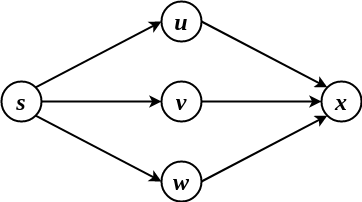
\includegraphics[width=0.6\textwidth]{images/radionet3.png}
    \caption{Controesempio in cui il protocollo \texttt{Flooding} non funziona.}
\end{figure}\label{fig:counterexampleflood}

Consideriamo il grafo nella \autoref{fig:counterexampleflood}, e supponiamo che la sorgente sia il nodo $s$. Al time slot $t_0$ la sorgente $s$ invierà il messaggio ai nodi $u,v,w$ e al time slot successivo i nodi $u,v,w$ invieranno il messaggio al nodo $x$, causando un interferenza. Dopo che $u,v,w$ avranno trasmesso, essi entreranno nello stato \texttt{done} e non trasmetteranno mai più. Così facendo il nodo $x$ non riceverà \textbf{mai} il messaggio, e il task non sarà mai risolto.

\subsection{Round-Robin Protocol}

Assumiamo che i nodi siano univocamente identificati da un valore nell'intervallo $[1,n]$, e ciascun nodo è a conoscenza della propria etichetta. Assumiamo inoltre che tutti i nodi conoscano una \textbf{buona approssimazione} di $n$. Per semplicità al momento assumiamo che conoscoano il valore esatto di $n$.

L'idea del protocollo \texttt{Round-Robin (RR)} è quella di scandire il protocollo in \textbf{fasi} con durata complessiva di $n$ time slots ciascuna. Dato che ogni fase $k \geq 0$ dura esattamente $n$ istanti, ogni nodo con etichetta $i$ trasmetterà al time slot $i-$esimo della fase $k$. Più formalmente, per ogni fase $k \geq 0$, il nodo $i$ può trasmettere solo negli istanti $kn + i$. Importante osservare che è possibile definire una scansione temporale delle azioni da svolgere grazie all'assunzione di sincronismo del sistema. Questo sistema ci garantisce che non è possibile che accada una situazione d'interferenza, in quanto può trasmetere un solo nodo alla volta.

\begin{algorithm}
\caption{Round-Robin Protocol}
\begin{algorithmic}[1]
\For{phase $j = 0, 1, 2, \dots$}
    \For{time $= jn, jn+1, \dots, (j+1)n-1$}
        \If{$id(x) \equiv \text{time} \pmod n\ \land$ state(x) = \texttt{informed}}
            \State \texttt{send(msg)}
            \State state(x) $\gets$ \texttt{done}
        \EndIf
    \EndFor
\EndFor
\end{algorithmic}
\end{algorithm}

\textbf{Osservazione:} Per come è definito il protocollo, questo non termina mai. Si mostrerà nell'analisi del protocollo che è sufficiente eseguire $n$ fasi.

\subsection{Analisi Round-Robin}

\begin{teorema}[Correttezza]
    Sotto le precedenti assunzioni, nel protocollo \texttt{RR}, tutti i nodi a distanza $k$ (distanza nel numero di archi, non euclidea) dalla sorgente $s$ verranno informati \textbf{entro} $k$ fasi.
    \begin{proof}
        Dimostriamo per induzione su $k$.
        \begin{description}
            \item[Passo Base] Nella prima fase, il primo nodo a trasmattere sarà la sorgente $s$ nel time slot $id(s)$; inoltre, in tale time-slot $s$ è l'unico nodo a trasmettere. Allora tutti i vicini di $s$ nel grafo delle comunicazioni, ossia i nodi a distanza 1 da $s$, per via del modello radio network, ricevono correttamente il messaggio.
            \item[Passo Induttivo] Supponiamo quindi per ipotesi induttiva che sia vero che per ogni fase $k > 0$ ogni nodo nell'insieme
            \[
                L_k := \{v \in V: d(s, v) = k\}
            \]
            (ovvero i nodi a distanza esattamente $k$ dalla sorgente) verrà informato entro la fine della fase $k$.

            Consideriamo ora un qualsiasi nodo $w \in L_{k+1}$. Per definizione di $L_{k+1}$, esiste \textbf{almeno} un nodo $v \in L_k$ tale che esista l'arco diretto $(v, w)$. Per ipotesi iduttiva, sappiamo che entro la fine della fase $k$ il nodo $v$ è stato informato. Se $v$ ha ricevuto il messaggio in un time slot $kn + i < kn + id(v)$, allora $v$ può trasmettere durante la fase $k$ stessa al tempo $kn + id(v)$, altrimenti se ha ricevuto il messaggio a un time slot $kn + i > kn + id(v)$, allora $v$ trasmetterà certamente nella fase $k + 1$, più precisamente al time slot $(k+1)n + id(v)$. In ogni caso, per definizione del protocollo \texttt{RR}, sia che $v$ trasmetterà al tempo $kn + id(v)$ oppure al tempo $(k+1)n + id(v)$, sarà l'unico che in quel momento invierà il messaggio a $w$. Perciò possiamo affermare che $w$ riceverà almeno una volta il messaggio senza alcuna interferenza, e questo vale per ogni $w \in L_{k+1}$.
        
            Infine, per ipotesi di connettività di $G$, vale che per ogni nodo $x \in V$, esiste un intero $h$ tale che $x \in L_h$.
        \end{description}
    \end{proof}
\end{teorema}

\begin{definizione}[Eccentricità]
    Definiamo l'eccentricità di un nodo $v \in V$ in un grafo connesso $G$ come la massima distanza tra $v$ e qualsiasi altro nodo del grafo. 
    \[
        \forall v \in V, \qquad e(v) := \max_{u \in V}d(v, u)
    \]
    Misura quanto un nodo è \textit{lontano} dal nodo più distante, definendo il raggio (eccentricità minima) e il diametro (eccentricità massima)
\end{definizione}

\begin{definizione}[Diametro]
    Il diametro in un grafo (connesso) è la massima distanza tra le coppie di nodi, definita come la lunghezza (numero di archi) del più lungo cammino minimo fra tutte le possibili coppie di vertici
    \[
        diam(G) = \max_{u,v \in V} d(u,v) = \max_{v \in V} e(v)
    \]
\end{definizione}

\begin{teorema}[Time Complexity]
    Sia la rete $G$ con $n$ nodi e sorgente $s$ di eccentricità $D = e(s)$. Sotto le precedenti assunzioni, il protocollo \texttt{RR} \textbf{completerà} il suo task in esattamente $nD \in O(n^2)$ time slots e tutti i nodi \textbf{termineranno} l'esecuzione del protocollo in $O(n^2)$ time slots.
    \begin{proof}
        Sia $D := e(s)$. Sicuramente in $D$ fasi tutti i nodi della rete verranno informati grazie al protocollo \texttt{RR}. Il problema è che nessun nodo conosce nè l'eccentricità di $s$, ne il diametro della rete. Però è noto che in una rete connessa di $n$ nodi, il diametro è \textbf{al più} $n - 1$. Perciò, dato che ogni nodo conosce il valore $n$, ognuno può stabilire che entro al \textbf{al più} $n-1$ fasi tutti i nodi saranno informati, e quindi potranno \textit{terminare} l'esecuzione del protocollo.
    \end{proof}
\end{teorema}

\begin{teorema}[Message Comeplixity]
    La message complexity del protocollo \texttt{RR} è 
    \[
        MSG[\texttt{RR}] = |E|.
    \]
    \begin{proof}
        Ogni nodo trasmetterà lungo tutti i suoi archi uscenti una volta sola il messaggio, perciò la message complexity sarà pari al numero di archi del grafo di trasmissione.
    \end{proof}
\end{teorema}

\section{Generalized Round-Robin Protocol}

Fin ora abbiamo assunto che tutti i nodi hanno una conoscenza di $n$, oppure una suo \textit{buona approssimazione}. Per esempio, se tutti i nodi avessero come approssimazione di un valore del tipo $3.5n$, l'efficienza del protocollo \texttt{RR} in termini asintotici non cambia.

Supponiamo ora invece che i nodi abbiano un'approssimazione $N$ del numero di nodi $n$. Col protocollo \texttt{RR} il tempo di terminazione globale sarà $O(N^2)$. Purtroppo però, se $N \in O(n^2)$, il tempo di terminazione del protocollo sarà dell'ordine di $O(n^4)$, o peggio ancora se $N \in O(2^n)$, il tempo di terminazione sarà $O(2^{2n})$, che è \textbf{molto elevato!}

Supponiamo in maniera ancora più generale che i nodi nella rete non conoscano affatto $n$ nè una sua approssimazione. Generalmente, in questi casi in cui non si conoscono alcuni parametri importanti per il problema, si ricorre alla tecnica della \textbf{simulazione}, in cui si provano tutti i possibili valori che i parametri mancanti possono assumere.

In questo caso quindi, dato che stiamo in un sistema totalmente sincrono, si eseguirà per prima cosa il protocollo \texttt{RR} supponendo che $n$ sia pari ad 1, poi si ripete supponendo che sia uguale a 2, e così via $\dots$. Così facendo, esisterà un tempo $t$ nel quale verrà eseguito il protocollo col corretto valore di $n$, portando a termine così il task del broadcast su reti radio.

\begin{algorithm}
\caption{Generalized Round-Robin Protocol}
\begin{algorithmic}[1]
\For{stage $k = 1, 2, \dots$}
    \For{phase $j = 0, 1, 2, \dots, k$}
        \For{time $= jk, jk+1, \dots, (j+1)k-1$}
            \If{$id(x) \equiv \text{time} \pmod k\ \land$ state(x) = \texttt{informed}}
                \State \texttt{send(msg)}
                \State state(x) $\gets$ \texttt{done}
            \EndIf
        \EndFor
    \EndFor
\EndFor
\end{algorithmic}
\end{algorithm}

Importante specificare però, che qualaora un nodo abbia un etichetta $x$ \textbf{maggiore} del corrente valore di $n$, esso non dovrà mai essere in grado di trasmettere il messaggio, in quanto potrebbe esistere un altro nodo con etichetta $y \geq n$ tale che $x \equiv_{n} y$, e quindi potrebbero occorrere interferenze.

In questo caso il task verrà completato in un tempo dell'ordine di
\[
    T = \sum_{i=1}^{n}T[\texttt{RR}(i)] = \sum_{i = 1}^{n} \Theta(n^2) \in \Theta(n^3)
\]

\subsection{Terminazione Locale}

Consideriamo il nodo $v_j$ con etichetta $j := id(v_j)$, e si consideri l'esecuzione del protocollo di \texttt{RR}$(n = i)$ in cui $v_j$ viene informato. Se abbiamo che $j < i$, sappiamo che se siamo fortunati, $v_j$ trasmetterà il messaggio direttamente nella fase $i$, altrimenti dovrà aspettare la fase successiva $i + 1$. Se invece $j > i$, allora sappiamo che $v_j$ non parlerà mai nella simulazione \texttt{RR}$(n = i)$. Esisterà comunque un tempo $i^* \geq j$ in cui $v_j$ avrà opportunità di trasmettere il messaggio ai suoi vicini.

In entrambi i casi, per come è costruito il protocollo, sappiamo che quando $v_j$ trasmetterà non ci potranno essere altri nodi che trasmettono nello stesso istante. Perciò $v_j$ informerà tutti i suoi vicini senza interferenze, e potrà concludere localmente il suo compito, passando nello stato \texttt{done}.

\subsection{Ottimizzazione}

Una ottimizzazione abbastanza intuitiva è quella di non far crescere il valore simulato di $n$ in maniera lineare, bensì in maniera \textit{esponenziale}. Ovvero, iteriamo le simulazioni del protocollo \texttt{RR} ponendo il parametro $n = 2^i,\ \forall i > 0$.

\begin{algorithm}
\caption{Optimized Generalized Round-Robin Protocol}
\begin{algorithmic}[1]
\For{stage $i = 1, 2, \dots$}
    \State $k \gets 2^i$
    \For{phase $j = 0, 1, 2, \dots, k$}
        \For{time $= jk, jk+1, \dots, (j+1)k-1$}
            \If{$id(x) \equiv \text{time} \pmod k\ \land$ state(x) = \texttt{informed}}
                \State \texttt{send(msg)}
                \State state(x) $\gets$ \texttt{done}
            \EndIf
        \EndFor
    \EndFor
\EndFor
\end{algorithmic}
\end{algorithm}

Per quanto riguarda il completamento del \textit{task}, esisterà certamente un certo $i$ tale che $2^{i-1} < n < 2^i$, garantendo quindi che entro $2^i$ simulazioni tutti i nodi verranno informati.

Per il tempo di terminazione invece, bata osservare che ci saranno al più $\lceil \log_2 n \rceil$ simulazioni, ognuna delle quali con complessità temporale di $O(n^2)$. Perciò avremo che
\[
    T = \sum_{i=1}^{\lceil \log_2 n \rceil}T[\texttt{RR}(i)] = \sum_{i = 1}^{\lceil \log_2 n \rceil} O(n^2 \log n) \in o(n^3)
\]

\section{Selective Protocol \& Lower Bound}

Introduciamo ora un nuovo protocollo deterministico. Innazitutto osserviamo che \texttt{RR} non sfrutta il parallelismo. Possono esistere nodi che anche se trasmittessero in contemporanea, non creerebbero interferenze. L'obiettivo è quello di progettare un algoritmo che possa selezionare le trasmissioni parallele.

\begin{definizione}[Famiglia $(n-k)$-selettiva]
    Dato $[n] = \{1, 2, \dots, n\}$ e dato $k \leq n$, una famiglia di sottoinsiemi
    \[
        \mathcal{H} = \{ H_1, H_2, \dots, H_t \}
    \]
    è detta $\mathbf{(n,k)}$\textbf{-selective} se, \textit{per ogni} sottoinsieme $S \subseteq [n]$ tale che $|S| \leq k$, esiste almeno un $H_i \in \mathcal{H}$ tale che
    \[
        |S \cap H_i| = 1
    \]
\end{definizione}

\textbf{Osservazione.} La famiglia 
\[
    \mathcal{H^{\text{singleton}}} = \{ \{1\}, \{2\}, \dots, \{n\} \}
\]
è una famiglia $\mathbf{(n,k)}$\textbf{-selective per ogni }$\mathbf{k}$. Questa famiglia singleton non ci piace, in quanto $t = n$ e noi vogliamo una famiglia con $t \leq n$.

\begin{teorema}[ClementiMontiSilvestri]
    Per $n$ sufficientemente grande e $k \leq n$, esiste una famiglia $\mathbf{(n,k)}$\textbf{-selective} di size $t \in O(k \log n)$ ed è ottimale.
\end{teorema}

Consideriamo il seguente protocollo che fa uso di una famiglia $\mathbf{(n,k)}$\textbf{-selective} per il task del broadcast nelle radio networks. Sia
\[
    \mathcal{H} = \{ H_1, H_2, \dots, H_t \}
\]
una famiglia $\mathbf{(n,d)}$\textbf{-selective} dove $d = \max_{v \in V} \delta(v)$, ossia è il grado massimo nel grafo $G$. Ciascun nodo, inoltre, conosce sia $n$ che $d$, oltre ad essere a conoscenza della famiglia $\mathcal{H}$.

\begin{algorithm}
\caption{Selective Protocol}
\begin{algorithmic}[1]
\For{phase $j = 0, 1, 2, \dots$}
    \For{time $t = 0, 1, \dots, j$}
        \For{each node $x \in H_j$}
            \If{$\text{state}(x) = \texttt{informed}$}
                \State \texttt{send(msg)}
            \EndIf
        \EndFor
    \EndFor
\EndFor
\end{algorithmic}
\end{algorithm}

Analizziamo ora questo protocollo. Vale il seguente lemma:
\begin{lemma}\label{lemma:select}
    Dopo la fase $j$, tutti i nodi a distanza al più $j$ saranno informati.
    \begin{proof}
        La dimostrazione è per induzione su $j$. Sia $s$ la sorgente e consideriamo il grafo di una visita BFS. Definiamo il livello $j$-esimo della BFS come segue:
        \[
            L_j = \{x \in V: d(s, x) = j\}
        \]
        \begin{description}
            \item[Passo Base] Sia $j = 0$. In questo caso solo la sorgente è informata e di conseguenza sarà l'unica a trasmettere.
            \item[Passo Induttivo] Sia $y \in L_j$. Consideriamo il sottoinsieme   
            \[
                N(y) = \{ x \in V:\ (x,y) \in E \land\ x \in L_{j-1} \}
            \]
            ossia tutti i vicini di $y$ a distanza $j-1$ dalla sorgente.
            \begin{figure}[h]
                \centering
                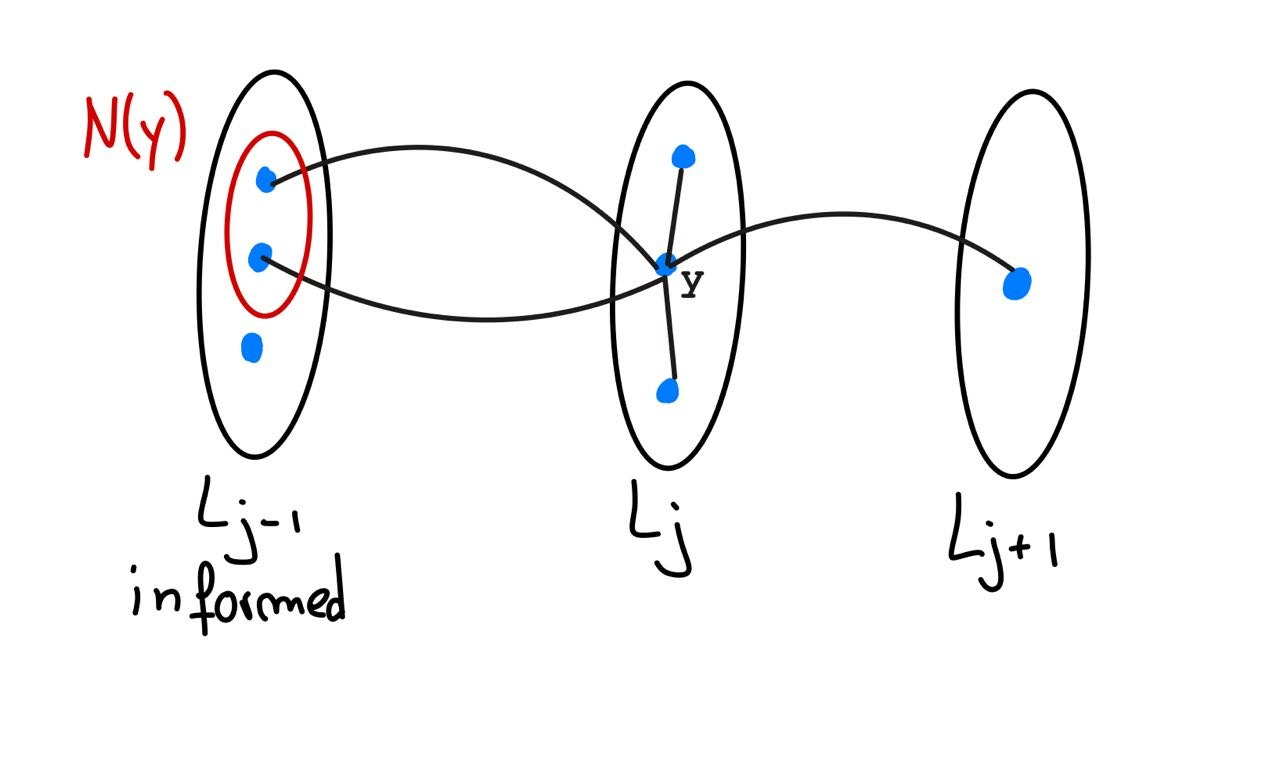
\includegraphics[width=0.6\textwidth]{images/lowerboundRadioNet1.jpg}
                \caption{Per ipotesi induttiva, tutti i nodi a distanza $L_{j-1}$ sono \texttt{informed}.}
            \end{figure}\label{fig:lowerboundRadioNet1}

            Come prima osservazione, notiamo che $N(y) \subseteq V$ e $|N(y)| \leq d$. Poiché $\mathcal{H}$ è una famiglia $(n,d)$-selettiva, per ogni insieme $S \subseteq V$ con $|S| \leq d$ esiste un indice $i \in [t]$ tale che $|S \cap H_i| = 1$. In particolare, questo vale per $S = N(y)$, dunque esiste un time slot $i$ tale che $|N(y) \cap H_i| = 1$.
        \end{description}
    \end{proof}
\end{lemma}

Tuttavia, sorge un problema: la definizione di famiglia selettiva garantisce solo l'esistenza di un $H_i$ tale che esattamente un nodo di $N(y)$ appartiene ad $H_i$, ma non ci dice chi è questo nodo.

\begin{figure}[h]
\centering
\begin{subfigure}[b]{0.48\textwidth}
    \centering
    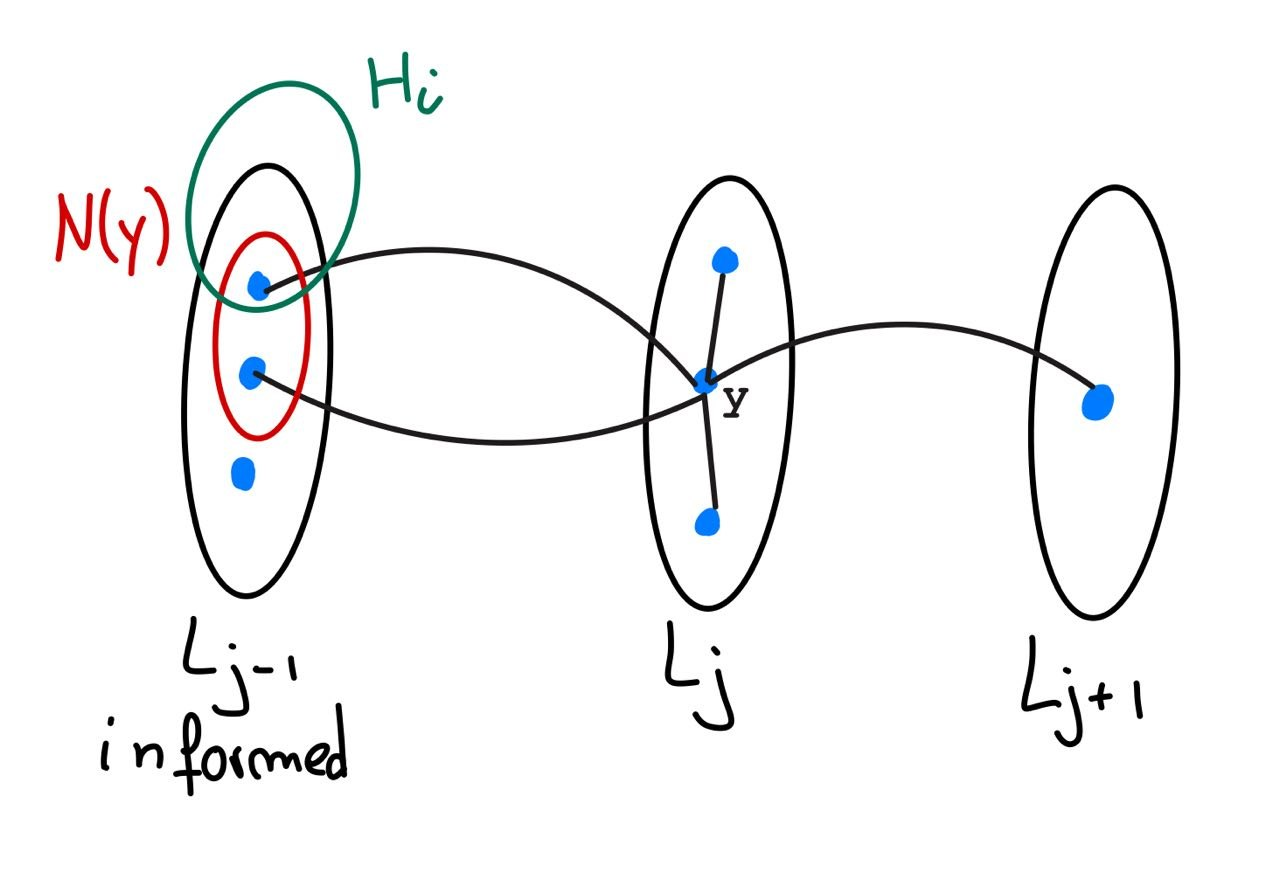
\includegraphics[width=\textwidth]{images/lowerboundRadioNet2.jpg}
    \caption{Caso favorevole.}
    \label{fig:lowerboundRadioNet12}
\end{subfigure}
\hfill
\begin{subfigure}[b]{0.48\textwidth}
    \centering
    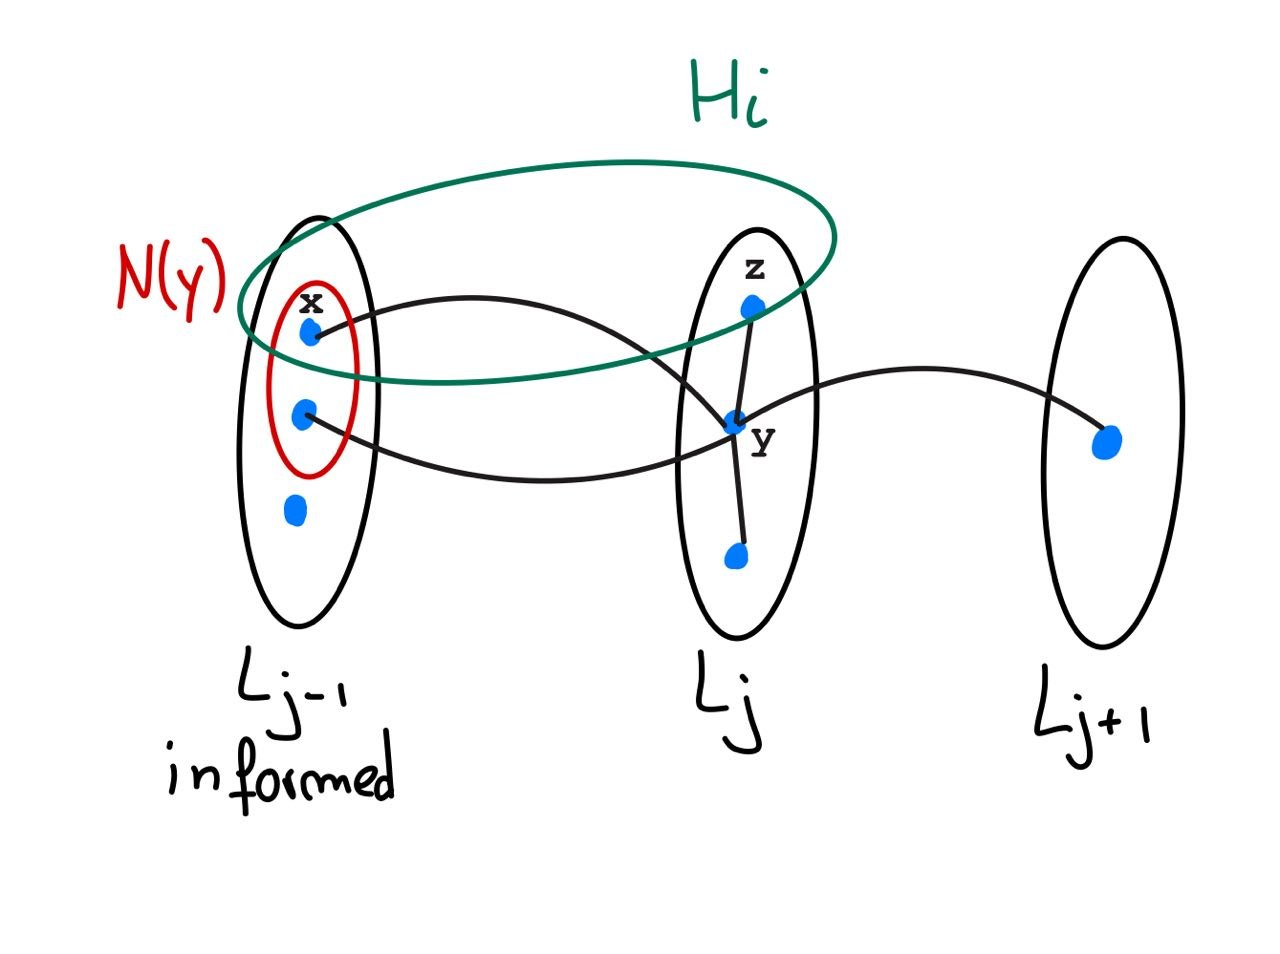
\includegraphics[width=\textwidth]{images/lowerboundRadioNet3.jpg}
    \caption{Caso non favorevole.}
    \label{fig:lowerboundRadioNet3}
\end{subfigure}
\caption{Confronto tra caso favorevole, quando viene scelto un nodo in $N(y)$ informato e caso non favorevole.}
\label{fig:lowerboundRadioNet}
\end{figure}

Il problema risiede nei nodi informati al livello $L_j$ \textbf{durante} la fase $j$. Sia $z \in L_j$ un tale nodo, come illustrato nella \autoref{fig:lowerboundRadioNet3}. Si presentano due casi critici:

\begin{enumerate}
\item Se includiamo $z$ in $N(y)$, la famiglia selettiva potrebbe sceglierlo come unico nodo attivo nell'intersezione $N(y) \cap H_i$, ma poiché $z$ non è ancora informato durante la fase $j$, non trasmetterà alcun messaggio.
\item Se escludiamo $z$ da $N(y)$, esso potrebbe comunque essere già informato e trasmettere simultaneamente ad altri nodi, generando \textbf{collisioni} su $y$.
\end{enumerate}

In entrambi i casi il protocollo fallisce. La soluzione è imporre che durante la fase $j$ siano \textbf{attivi} esclusivamente i nodi che sono stati informati nella fase $j-1$: in questo modo si garantisce che ogni nodo attivo sia effettivamente informato e pronto a trasmettere, eliminando sia il problema della mancata trasmissione sia quello delle collisioni.

Con questa modifica al protocollo, ora il \autoref{lemma:select} è valido, quindi dopo $D$ fasi, tutti i livelli saranno informati. Quindi il tempo di completamento è:
\[
    T = O(D |\mathcal{H}|) = O(D \cdot d \log n)
\]
dove $D = diam(G)$. Dunque, per $D$ e $d$ piccoli, otteniamo un tempo di completamento migliore rispetto al protocollo \texttt{Round-Robin}. Il teorema successivo ci dice inoltre che non possiamo fare di meglio.

\begin{teorema}[Lower Bound]
    Dato un grafo diretto di trasmissione $G=(V,E)$ relativo ad una rete wireless, con diametro $D$, grado massimo $\Delta$ tale che $D\Delta < n$, allora esiste sempre un modo di manipolare i ritardi in modo tale che non si possa risolvere il problema del broadcasting a singola sorgente in un tempo migliore di
    \[
        \Omega(D\Delta \log\left(\frac{n}{D}\right))
    \]
a meno che non si assuma che tutti i nodi conoscano un famiglia $(n,\Delta)$-selettiva di $V$.
\end{teorema}

Per esempio, se consideriamo un grafo con un diametro costante, per esempio $D=3$, avremo che il grado massimo dei nodi $\Delta$ crescerà molto velocemente al crescere di $n$, per esempio in maniera lineare $(\Delta \in O(n))$. Perciò in questo caso avremo un lowerbound di $\Omega(n \log n)$.

Quello che ci si chiede è se esiste un modo per abbattere il fattore $\Delta$ dal lowerbound. Il teorema precedentemente enunciato ci dice che questo è \textbf{deterministicamente} impossibile, perciò è necessario occorrere alla \textit{randomness}.

\section{Probabilistic Protocol}

Definiamo un protocollo probabilistico molto semplice, in cui ogni nodo informato trasmette ai suoi vicini con una certa probabilità $p$ fissata uguale per tutti. È facile mostrare con un controesempio in cui il tempo medio di completamento del protocollo è pessimo.

\begin{figure}[h]
    \centering
    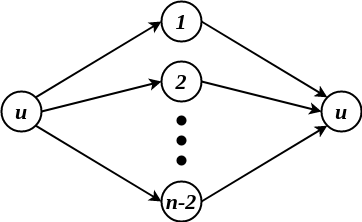
\includegraphics[width=0.4\textwidth]{images/radionet4.png}
    \caption{Controesempio.}
\end{figure}\label{fig:controesempio}

Sia la $u$ la sorgente. Sicuramente esiste un tempo $t_0$ in cui $u$ trasmette il messaggio a tutti i suoi vicini $1, 2, \dots, n-2$ senza interferenze. Dal time slot successivo tutti i suoi vicini inizieranno a trasmettere verso $v$, ognuno con probabilità $p$. Supponiamo per esempio che $p = \frac{1}{2}$, e cerchiamo di stabilire entro quanto tempo ci si aspetta che $v$ verrà informato senza alcuna interferenza. Per prima cosa dobbiamo calcolare con quale probabilità l'evento 
\[
    \mathcal{E} = "v \texttt{ viene informato}"
\]
occorre, e questo si può fare usando la distribuzione binomiale
\[
    P(\mathcal{E}) = \binom{n-2}{1}\frac{1}{2}\left(\frac{1}{2}\right)^{n - 3} = \frac{n-2}{2^{n-2}} \in \Theta\left(\frac{n}{2^n}\right)
\]

Ogni time slot rappresenta un tentativo indipendente in cui l'evento $\mathcal{E}$ ha probabilità $p$ di verificarsi. Aspettare il verificarsi del "primo successo" in una serie di tentativi indipendenti modella esattamente una \textbf{variabile aleatoria geometrica}. Il valore atteso di tale variabile è $1/p$. Si ottiene un tempo di attesa (di completamento del task) $\Theta\left(\frac{2^n}{n}\right)$, che cresce in modo esponenziale.

Anche se $v$ avesse molti meno vicini, per sempio $\sqrt{n}$, il tempo di completamento sarebbe comunque pessimo, $\Theta\left(\frac{2^{\sqrt{n}}}{\sqrt{n}}\right)$

Se inveve $v$ avesse solamente $2$ vicini che trasmettono, il protocollo terminerebbe in tempi brevissimi. Ciò ci suggerisce che dobbiamo trovare un valore di $p$ in modo tale che è \textbf{poco probabile} che avvengano interferenze, ovvero un valore per il quale \textbf{in media} trasmette un solo vicino di ogni nodo. Considerando sempre il precedente controesempio, il valore ottimale per $p$ per il quale i vicini di $v$ devono trasmettere è $\frac{1}{d^{in}(v)}$, ovvero il grado entrante di $v$.

\subsection{BGI Protocol on $d$-Regular Layered Graphs}

Come primo passo consideriamo grafi con strutture che in qualche modo ci semplificano il lavoro. Consideriamo grafi di tipo $d$\textbf{-regular layered}, ovvero grafi suddivisi in \textbf{strati} $L_1, L_2, \dots, L_D$ in cui esistono archi solamente da un livello a quello successivo, e in cui ogn nodo v ha un grado entrante costante a tutti pari a $d^{(in)(v)} = d$. Inoltre esiste una sorgente $s$ tale che $(s,v) \in E \forall v \in L_1$.


\begin{figure}[h]
    \centering
    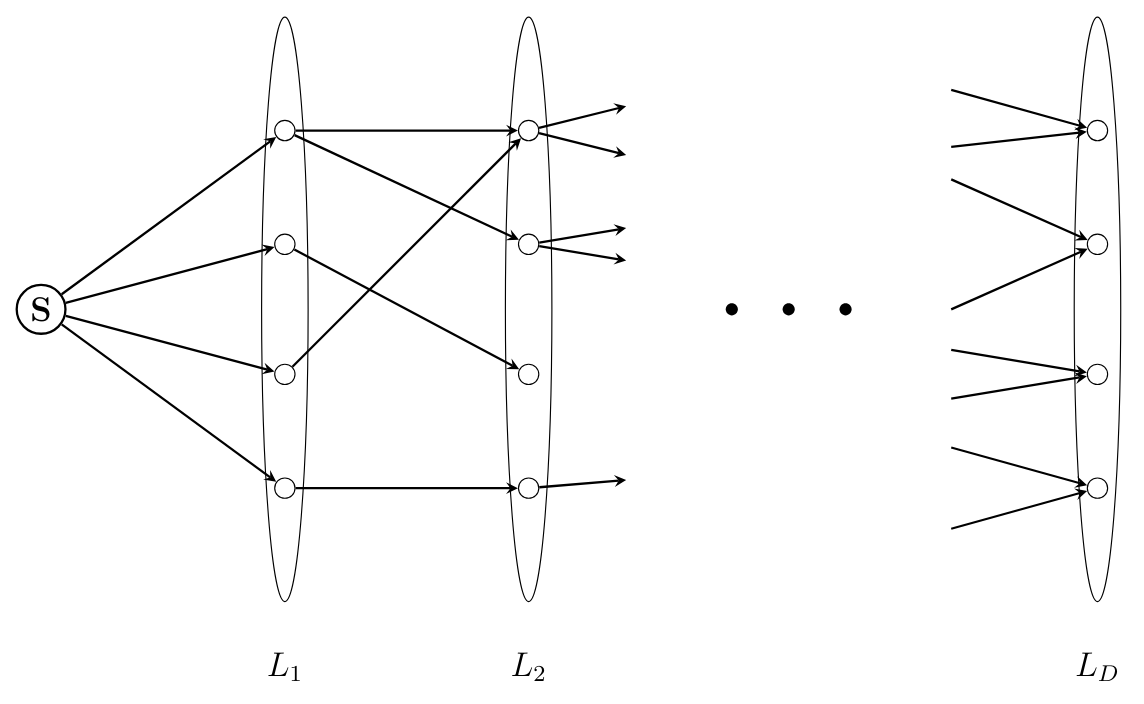
\includegraphics[width=0.4\textwidth]{images/radionet5.png}
    \caption{Esempio di $d$-regular}
\end{figure}\label{fig:dlayered}

Osservare che la descrizione appena data non è propriamente precisa, in quanto i nodi in $L_1$ hanno grado pari ad 1, e quindi non necessariamente $d$, mentre il grado entrante della sorgente $s$ è pari a 0.

\begin{algorithm}
\caption{BGI Protocol}
\begin{algorithmic}[1]
\If{state(x) = \texttt{source}}
    \State \texttt{send(msg)} with probability $p = 1$
\EndIf
\For{stage $k = 1, 2, \dots$}
    \For{time $t =1, 2, \dots, c\log n$}
        \If{$\text{state}(x) = \texttt{informed}$ in stage $k - 1$}
            \State \texttt{send(msg)} with probability $p = \frac{1}{d}$
        \EndIf
    \EndFor
\EndFor
\end{algorithmic}
\end{algorithm}

\begin{teorema}
    Il protocollo \texttt{BGI} su grafi $d$-regular e $D$ layered completa \textit{w.h.p.} il task del broadcast dalla sorgente $s$ in $O(D)$ stages e quindi in $O(D \log n)$ time slots.
    \begin{proof}
        La dimostrazione verrà fatta per induzione sui livelli $j = 1, 2, \dots, D$, ovvero si vuole dimostrare che al termine dello stage $j$ con alta probabilità tutti i nodi del livello $L_j$ saranno informati.

        Il caso per $j = 1$ è banale, perciò assumiamo come \textit{ipotesi iduttiva} che \textbf{con alta probabilità} entro la file dello stage $j > 1$ tutti i nodi nel livello $L_j$ sono già informati (ovvero entro $O(j \log n)$ time slots). Si vuole dimostrare che questo è vero anche per $j + 1$.

        Consideriamo quindi un nodo $v \in L_{j+1}$. Inziamo con calcolare la probabilità che $v$ viene informato in un dato time slot della fase $j+1$. Tale probabilità è pari alla probabilità che uno solo dei suo $d$ \textit{inner-neighbours} trasmette, mentre tutti gli altri $d-1$ non trasmettono, e ciò avviene con probabilità:
        \[
            \binom{d}{1}\frac{1}{d}\left(1 - \frac{1}{d}\right)^{d-1} = \frac{d}{d}\left(1 - \frac{1}{d}\right)^{d-1} = \left(1 - \frac{1}{d}\right)^{d-1}
        \]
        Per valori $d \geq 2$, la quantità $\left(1 - \frac{1}{d}\right)^{d-1} > \frac{1}{8}$ (non ha senso considerare $d = 1$).

        Proseguendo, possiamo dire che il nodo $v$ al livello $j + 1$ non viene informato in un time slot con probabilità al più $1 - \frac{1}{8}$. Quindi

        \begin{align*}
            P(v \text{ non informato in tutti i } c\log n  &\text{ time slot dello stage } j+1) \\
            &< \left(1 - \frac{1}{8}\right)^{c\log n} \\
            &< e^{-\frac{c}{8} \log n} \\
            &= \frac{1}{n^{c/8}}
        \end{align*}
        La prima disuguaglianza è vera perché ogni nodo trasmette in maniera totalmente indipendente dagli altri, mentre la seconda è data dalla seguente espressione
        \[
            1 - x < e^{-x} \quad \forall 0 < x < 1
        \]

        Quindi, se definiamo l'evento
        \[
            \mathcal{E}_v = v \text{ non informato in tutti i } c\log n  \text{ time slot dello stage } j+1
        \]
        occore con al più
        \[
            P(\mathcal{E}_v) \geq \frac{1}{n^{c/8}}
        \]
        Per \textbf{union bound}, possiamo dire che esiste \textbf{almeno un nodo} al livello $L_{j+1}$ che non viene informato entro la fine dello stage $j+1$ occorre con probabilità al più
        \[
            P\left(\cup_{v \in L_{j+1}} \mathcal{E}_v \right) \leq \sum_{v \in L_{j+1}}  P(\mathcal{E}_v) < n \frac{1}{n^{c/8}} = \frac{1}{n^{c/8 - 1}}
        \]
        A questo punto, ponendo $c = 16$, avremo che la probabilità di avere un cosidetto \textit{bad stage} in cui \textbf{non tutti} i nodi del relativo livello vengono informati è al più $\frac{1}{n}$. Possiamo quindi concludere dicendo che ogni nodo $v \in L_{j+1}$ viene informato entro la fine dello stage $j+1$ con probabilità \textbf{almeno} $1 - \frac{1}{n}$, dimostrando così il teorema.
    \end{proof}
\end{teorema}

\subsection{BGI Protocol on General Graphs}

\include{hashing}
\include{sampling}

\end{document}